\documentclass[10pt,twocolumn,letterpaper]{article}

\usepackage{eso-pic}
\usepackage{cvpr}
\usepackage{times}
\usepackage{epsfig}
\usepackage{graphicx}
\usepackage{amsmath}
\usepackage{amssymb}
\usepackage{xspace}
\usepackage{booktabs}
\usepackage{placeins}


% Include other packages here, before hyperref.
\usepackage{my_macros}
\usepackage{paralist}
\usepackage{amsthm}
% \usepackage{dirtytalk} fah: my miktex didn't like this; and we don't need it here. 
%\usepackage{framed}
\usepackage{caption}
\usepackage{subcaption}
\usepackage{algorithm}
%\usepackage{algorithmic}
\usepackage{algpseudocode}
\usepackage{setspace}
%for tikz
\usepackage{tikz,pgfplots}
\usepackage{pgfplotstable}
\usepackage{filecontents}
%\usepackage{scrextend}
\usepackage[pagebackref=true,breaklinks=true,letterpaper=true,colorlinks,bookmarks=false]{hyperref}
\pdfpageattr{/Group <</S /Transparency /I true /CS /DeviceRGB>>}
\usepackage{everypage}
\AddEverypageHook{%
  \makeatletter%
  \special{pdf: put @thispage <</Group << /S /Transparency /I true /CS /DeviceRGB>> >>}%
  \makeatother%
}%

\newcommand{\footlabel}[2]{%
    \addtocounter{footnote}{1}%
    \footnotetext[\thefootnote]{%
        \addtocounter{footnote}{-1}%
        \refstepcounter{footnote}\label{#1}%
        #2%
    }%
    $^{\ref{#1}}$%
}

\newcommand{\footref}[1]{%
    $^{\ref{#1}}$%
}
\usetikzlibrary{arrows,positioning,automata,shadows,fit,shapes}
\usetikzlibrary{arrows,petri,topaths}
\usetikzlibrary{positioning,fit,calc}
\usetikzlibrary{shapes.arrows,chains,decorations.pathreplacing,fadings}
\usetikzlibrary{calc, matrix, backgrounds}




%%%%%%global tikz styles
\tikzstyle{nS}=[circle,minimum size = 0.6cm,inner sep = 0pt,draw, font=\small,align=left]
\tikzstyle{eNS}=[fill=white,minimum size = 0.5cm,inner sep = 0pt, font=\tiny,align=left]

\tikzstyle{eBlack}=[very thick,minimum size = 0.5cm,inner sep = 0pt,draw=black!70!black, font=\small,align=left, line width=1mm]
\tikzstyle{eNotCut}=[very thick,minimum size = 0.5cm,inner sep = 0pt,draw=green!70!black, font=\small,align=left, line width=1mm]
\tikzstyle{eBlue}=[very thick,minimum size = 0.5cm,inner sep = 0pt,draw=blue!70!black, font=\small,align=left, line width=1mm]
\tikzstyle{eCut}=[very thick,dotted,minimum size = 0.5cm,inner sep = 0pt,draw=black, font=\small,align=left, draw=red!70!black, line width=1mm]

\pgfplotsset{every axis/.append style={
  every axis y label/.style = {at={(ticklabel cs:0.5)}, rotate=90, anchor=south},
  axis x line = {bottom},
  axis y line = {left},
  tick align = outside,
  ymajorgrids = true,
%  legend style = {draw=none, at={(1.05, 0.5)}, anchor=west, font=\small},
  legend style = {font=\tiny},
  legend columns = 1,
  every axis plot/.append style = {line width=1pt},
  label style = {font=\small},
  tick label style={font=\small},
  scaled ticks = false,
}}

% Two Colored Circle Split 
\makeatletter
\tikzset{circle split part fill/.style  args={#1,#2}{%
 alias=tmp@name, 
  postaction={%
    insert path={
     \pgfextra{% 
     \pgfpointdiff{\pgfpointanchor{\pgf@node@name}{center}}%
                  {\pgfpointanchor{\pgf@node@name}{east}}%            
     \pgfmathsetmacro\insiderad{\pgf@x}
      \fill[#1] (\pgf@node@name.base) ([xshift=-\pgflinewidth]\pgf@node@name.east) arc
                          (0:180:\insiderad-\pgflinewidth)--cycle;
      \fill[#2] (\pgf@node@name.base) ([xshift=\pgflinewidth]\pgf@node@name.west)  arc
                           (180:360:\insiderad-\pgflinewidth)--cycle;            
         }}}}}  
 \makeatother  

%\usepackage{tkz-berge}
\DeclareMathOperator*{\argmin}{arg\,min}
\DeclareMathOperator*{\argmax}{arg\,max}
\definecolor{shadecolor}{rgb}{0.01,0.199,0.1}
\usepackage{xargs} 
\newtheorem{theorem}{Theorem}
\newtheorem{remark}{Remark}
\theoremstyle{definition}
\newtheorem{definition}{Definition}

% If you comment hyperref and then uncomment it, you should delete
% egpaper.aux before re-running latex.  (Or just hit 'q' on the first latex
% run, let it finish, and you should be clear).
\usepackage{bm}% ändert \boldsymbol
\def\arraystretch{0.8}
\renewcommand{\tabcolsep}{2pt}
\newcommand{\thickline}{2pt}
\newcommand{\scatterplotpath}{./scatterplots/}
\newcommand{\rd}{\color{red}}

\usepackage[colorinlistoftodos,prependcaption,textsize=tiny]{todonotes}
\newcommandx{\unsure}[2][1=]{\todo[linecolor=red,backgroundcolor=red!25,bordercolor=red,#1]{#2}}
\newcommandx{\change}[2][1=]{\todo[linecolor=blue,backgroundcolor=blue!25,bordercolor=blue,#1]{#2}}
\newcommandx{\info}[2][1=]{\todo[linecolor=OliveGreen,backgroundcolor=OliveGreen!25,bordercolor=OliveGreen,#1]{#2}}
\newcommandx{\improvement}[2][1=]{\todo[linecolor=Plum,backgroundcolor=Plum!25,bordercolor=Plum,#1]{#2}}
\newcommandx{\thiswillnotshow}[2][1=]{\todo[disable,#1]{#2}}
\newcommand{\OR}{\textrm{ or }}

% \cvprfinalcopy % *** Uncomment this line for the final submission


\def\cvprPaperID{****} % *** Enter the CVPR Paper ID here
\def\httilde{\mbox{\tt\raisebox{-.5ex}{\symbol{126}}}}

\newcommand{\realplot}[1]{
\begin{tikzpicture}
    \begin{axis}
        \addlegendimage{empty legend}\addlegendentry{Matrix #1}
        \addplot {0};
        \addplot {1};
        \addplot {2};
        \addplot {3};
    \end{axis}
\end{tikzpicture}}  

% \newcommand{\anytimeplot}[1]{
%   \addplot[color=brown,mark=x] table[x=time,y=HC]{data3/knott-3d-300.data};              \addlegendentry{HC}
%   \addplot[color=black,mark=x] table[x=time,y=HC-CGC]{data3/knott-3d-300.data};          \addlegendentry{HC-CGC}
%   \addplot[color=red,mark=x] table[x=time,y=CGC]{data3/knott-3d-300.data};               \addlegendentry{CGC}
%   \addplot[color=gray,mark=o] table[x=time, y=ogm-KL]{data3/knott-3d-300.data};          \addlegendentry{KL}
%   \addplot[color=purple,mark=x] table[x=time, y=MCR-CCFDB]{data3/knott-3d-300.data};     \addlegendentry{MC-R}
%   \addplot[color=blue,mark=x] table[x=time, y=MCI-CCIFD]{data3/knott-3d-300.data};       \addlegendentry{MC-I}
%   \addplot[color=green,mark=x] table[x=time, y=DYNCC-HC-MC]{data3/knott-3d-300.data};    \addlegendentry{Fusion-HC-MC}
%   \addplot[color=cyan,mark=x] table[x=time, y=DYNCC-HC-CGC]{data3/knott-3d-300.data};    \addlegendentry{Fusion-HC-CGC}
%   \addplot[color=orange,mark=x] table[x=time, y=DYNCC-WS-MC]{data3/knott-3d-300.data};  \addlegendentry{Fusion-WS-MC}
%   \addplot[color=orange,mark=x] table[x=time, y=DYNCC-WS-CGC]{data3/knott-3d-300.data};  \addlegendentry{Fusion-WS-CGC}
% }
\newcommand{\anytimeplot}[1]{
  \addplot[color=brown,mark=x] table[x=time,y=HC]{data3/#1.data};              \addlegendentry{HC}
  \addplot[color=black,mark=square] table[x=time,y=HC-CGC]{data3/#1.data};          \addlegendentry{HC-CGC}
  \addplot[color=red,mark=x] table[x=time,y=CGC]{data3/#1.data};               \addlegendentry{CGC}
  \addplot[color=gray,mark=o] table[x=time, y=ogm-KL]{data3/#1.data};          \addlegendentry{KL} 
  \addplot[color=yellow!50!black,mark=square] table[x=time, y=ogm-mcfusion-HC-CF*]{data3/#1.data};  \addlegendentry{Fusion}
  \addplot[color=purple,mark=o] table[x=time, y=MCR-CCFDB]{data3/#1.data};     \addlegendentry{MC-R}
  \addplot[color=blue,mark=o] table[x=time, y=MCI-CCIFD]{data3/#1.data};       \addlegendentry{MC-I}
  \addplot[color=green,mark=o] table[x=time, y=DYNCC-HC-MC]{data3/#1.data};    \addlegendentry{CCFusion-HC-MC}
  \addplot[color=cyan,mark=x] table[x=time, y=DYNCC-HC-CGC]{data3/#1.data};    \addlegendentry{CCFusion-HC-CGC}
  \addplot[color=orange,mark=o] table[x=time, y=DYNCC-WS-MC]{data3/#1.data};  \addlegendentry{CCFusion-WS-MC}
  \addplot[color=pink,mark=x] table[x=time, y=DYNCC-WS-CGC]{data3/#1.data};  \addlegendentry{CCFusion-WS-CGC}
}
%  \addplot[color=yellow!50!black,mark=o] table[x=time, y=ogm-mcfusion-HC-CF*]{data3/#1.data};  \addlegendentry{Fusion}
  %\addplot[color=green!50,mark=o] table[x=time, y=PIVOT*]{data3/#1.data};          \addlegendentry{PIVOT-BOEM}

% Pages are numbered in submission mode, and unnumbered in camera-ready
\ifcvprfinal\pagestyle{empty}\fi
\begin{document}
%%%%%%%%% TITLE
%!TEX root = egpaper_for_review.tex
\newcommand{\Cut }{\mathcal{C}}
%\title{Correlation Clustering with Dynamic Super-Nodes (DySNCC)}
\title{Fusion Moves for Correlation Clustering}

\author{First Author\\
Institution1\\
Institution1 address\\
{\tt\small firstauthor@i1.org}
% For a paper whose authors are all at the same institution,
% omit the following lines up until the closing ``}''.
% Additional authors and addresses can be added with ``\and'',
% just like the second author.
% To save space, use either the email address or home page, not both
\and
Second Author\\
Institution2\\
First line of institution2 address\\
{\tt\small secondauthor@i2.org}
}

\maketitle
%\thispagestyle{empty}


%%%%%%%%% ABSTRACT
\begin{abstract}
  \color{red} \textbf{TODO:}
Correlation clustering, or multicut partitioning, is the NP-hard problem of partitioning an undirected graph or image with positive / attractive and negative / repulsive edge weights such that the sum of cut edge weights is minimized. We here present a move-making heuristic that uses cheaply generated proposal clusterings to iteratively and monotonously improve upon the best previously found clustering. A valid partitioning is maintained at all times, and solutions close to the global optimum are obtained faster than with any published technique. 
    
%We address the problem of partitioning a  graph
%   into a previously unknown number of clusters.
%   Among all partitions, the one with the minimal 
%   sum of of cut edge weights is chosen. 
%   This problem is known as correlation clustering 
%   or multicut.
%   We propose a general framework to find
%   high quality approximate solutions for 
%   this NP-hard problem based on a move making algorithm:
%   We use candidate solutions from a proposal generator
%   to iteratively improve the best observed solution similar
%   to fusion moves.
%   The proposed solver outperforms any other solver
%   w.r.t. to any time performance.
%   The solutions found by this solver are close
%   to global optimal solutions w.r.t. energy
%   and problem specific measurements as VI for
%   image segmentation problems.

\end{abstract}

%!TEX root = ./egpaper_for_review.tex
%
\section{Introduction}
Correlation clustering~\cite{Bansal-2002}, also known as the multicut problem~\cite{chopra_1993_mp} 
is a basic primitive in computer vision~\cite{andres_2011_iccv,kroeger_2012_eccv,yarkony_2012_eccv,alush_2013_simbad} and data mining~\cite{Arasu-2009,Sadikov-2010,Chen-2012,Chierichetti-2014}.
See Sec.~\ref{sec:problem_formulation} for its formal definition of clustering the nodes of a graph.
 
Its merit is, firstly, that it accommodates both positive (attractive) \emph{and} negative (repulsive) edge weights.
This allows doing justice to evidence in the data that two nodes or pixels do not wish or do wish to end up in the same cluster or segment, respectively.
Secondly, it does not require a specification of the number of clusters beforehand.


In signed social networks, where positive and negative edges encode friend and foe relationships, respectively,
correlation clustering is a natural way to detect communities~\cite{Chen-2012,Chierichetti-2014}.
Correlation clustering can also be used to cluster query refinements in web search~\cite{Sadikov-2010}.
Because social and web-related networks are often huge, heuristic methods, \eg the PIVOT-algorithm~\cite{Ailon-2008},
are popular~\cite{Chierichetti-2014}.

In computer vision applications, unsupervised image segmentation algorithms often start with an over-segmentation
into superpixels (superregions), which are then clustered into ``perceptually meaningful''
regions by correlation clustering.
Such an approach has been shown to yield
state-of-the-art results on the Berkeley Segmentation Database
\cite{andres_2011_iccv,Kim-2011,yarkony_2012_eccv,alush_2013_simbad}.

While it has a clear mathematical formulation and nice properties,
correlation clustering suffers from NP-hardness. 
%
Consequently, partition problems on large scale data, \eg
huge volume images in computational neuroscience~\cite{kroeger_2012_eccv}
or social networks~\cite{Leskovec-2010}, 
are not tractable because reasonable solutions cannot be computed in acceptable time.

% Importantly, this allows doing justice to evidence in the data that two nodes or pixels do \emph{not} wish to end up in the same cluster or segment. This is in contrast to the submodular potentials so popularized by the graph cut algorithm, which only allow two nodes to be attracted to each other, or at most be agnostic about membership in the same cluster. Secondly, the algorithm does not require a specification of the number of clusters. This is in contrast to methods such as normalized cut \cite{} that can only accommodate attractive interactions and hence need the number of clusters to be specified. 

% \paragraph{Contribution.} The evident usefulness of correlation clustering and its clean and compact formulation in terms of an optimization problem, together with its unfortunate NP-hardness, are an invitation to develop fast approximate solvers. The basic idea of the move making algorithm proposed here is to maintain, at all times, a best current partitioning; and to iteratively improve it (as we show, monotonously) by considering diverse and cheaply generated proposal partitionings. Any two nodes that are in one cluster in both the current and the proposal partitioning are contracted. Edges to contracted nodes are equally combined and reweighted, and the correlation clustering problem is then solved on this reduced graph. We offer a polyhedral characterization of this strategy, and evaluate it in conjunction with two versatile proposal generators.   We conduct experiments on a broad range of data sets ranging from 2D and 3D segmentation problems to clustering in signed social networks. The results suggest that this simple move making algorithm is the fastest technique known today, reaching close to globally optimal solutions in a tenth or a hundredth of the time required by the most efficient exact solvers. 
\vspace{0.1cm}
\noindent \textbf{Contribution.}
In this work we present novel approaches that are designed for large scale correlation clustering problems.
First, we define a novel energy based agglomerative clustering algorithm that monotonically increases the energy.
With this at hand we show how to improve the anytime performance of Cut, Clue \& Cut~\cite{beier_2014_cvpr}.
%
Second, we improve the anytime performance of polyhedral multicut methods~\cite{kappes_2013_arxiv} by more efficient separation procedures.
%
Third, we introduce cluster-fusion moves, which extend the original fusion moves~\cite{Lempitsky-2010} 
used in supervised segmentation to the unsupervised case and give a polyhedral interpretation of this algorithm.
Finally, we propose two versatile proposal generators, and evaluate the proposed methods on existing and new benchmark problems.
Experiments show that we can improve the computation time by one to two magnitudes without worsening the segmentation 
quality significantly.
 
\vspace{0.1cm}
\noindent \textbf{Related Work.}
A natural approach is to solve the integer linear program (ILP) directly~\ref{eq:edgeproblem}. 
To this end, efficient separation procedures have been found~\cite{kappes_2011_emmcvpr,kappes_2013_arxiv} that allow to iteratively augment the set of constraints until a valid partitioning is found. 
Alternatively, it is possible to relax the integrality constraints of the ILP formulation~\cite{kappes_2013_arxiv}. 
Such an outer relaxation can be iteratively tightened. However, intermediate solutions are fractional and therefore rounding is required to obtain a valid partitioning.
For the latter approach column generating methods exist, which work best on planar graphs~\cite{yarkony_2012_eccv}. %or almost planar \cite{yarkony-andres-2013} graphs. 

Another line of work uses move making algorithms 
to optimize correlation clustering~\cite{Kernighan-1970,bagon_2011_arxiv,beier_2014_cvpr}.
Starting with an initial segmentation, auxiliary max-cut problems are (approximately) solved,
such that the segmentation is strictly improved.
As shown in~\cite{beier_2014_cvpr} only Cut, Glue \& Cut (CGC)
can deal with large scale problems, but can also suffer from very large auxiliary problems.

Outside computer vision, greedy methods~\cite{Soon-2001,Ng-2002,Gionis-2007,Elsner-2008,Ailon-2008} have been suggested for correlation clustering problems, see \cite{Elsner-2009} for an overview.
The PIVOT Algorithm~\cite{Ailon-2008} iterates over all nodes in random order.
If the node is not assigned it constructs a cluster containing the node and all its 
unassigned positively linked neighbors.  
%
A widely used post-processing method is  Best One Element Move (BOEM)~\cite{Gionis-2007}, which iteratively reassigns nodes to clusters.

For energy minimization problems fusion moves have become increasingly popular~\cite{Lempitsky-2010,kappes_2014_ws}.
For many large scale computer vision applications fusion moves lead to good approximations
with state of the art anytime performance~\cite{kappes_2014_ws}.
Due to the ambiguity of a node-labeling, classical fusion moves~\cite{Lempitsky-2010} cannot be applied directly for correlation clustering.
We will show how to overcome this problem in Sec.~\ref{sec:cc_fm}.


\vspace{0.1cm}
\noindent \textbf{Outline:} 
In Sec.~\ref{sec:problem_formulation} we give a 
detailed problem definition and introduce 
the correlation clustering objective.
Next we give a description of energy based hierarchical clustering in Sec.~\ref{sec:ehc} and
our proposed correlation clustering fusion moves in Sec.~\ref{sec:cc_fm}.
We evaluate the proposed methods in Sec.~\ref{sec:exp} and conclude in Sec.~\ref{sec:future} and \ref{sec:conclusion}.

%-------------------------------------------------------------------------

%!TEX root = ../egpaper_for_review.tex
%
%\tikzstyle{nS}=[circle,minimum size = 0.6cm,inner sep = 0pt,draw, font=\small,align=left]
%\tikzstyle{eNS}=[fill=white,minimum size = 0.5cm,inner sep = 0pt, font=\tiny,align=left]
% size = 0.5cm,inner sep = 0pt,draw=black, font=\small,align=left, draw=red!70!black, line width=1mm]
%
\begin{center}
\begin{figure}[t]
\begin{tiny}
\begin{subfigure}[t]{0.22\linewidth}
    \resizebox{\linewidth}{!}{
        \begin{tikzpicture}[scale=1]%[x=1 cm, y=1 cm]
                \draw (2,2) node[nS,fill=red!60] (n0) {$0$}; 
                \draw (4,2) node[nS,fill=red!60] (n1) {$1$};
                \draw (6,2) node[nS,fill=blue!60] (n2) {$2$};
                \draw (2,0) node[nS,fill=red!60] (n3) {$3$}; 
                \draw (4,0) node[nS,fill=red!60] (n4) {$4$};
                \draw (6,0) node[nS,fill=green!60] (n5) {$5$};
                \path
                    (n0) edge[eBlack] node[eNS]{$w_{01}$} (n1) 
                    (n1) edge[eBlack] node[eNS]{$w_{12}$} (n2) 
                    (n3) edge[eBlack] node[eNS]{$w_{34}$} (n4) 
                    (n4) edge[eBlack] node[eNS]{$w_{45}$} (n5)
                    (n0) edge[eBlack] node[eNS]{$w_{03}$} (n3)
                    (n1) edge[eBlack] node[eNS]{$w_{14}$} (n4)
                    (n2) edge[eBlack] node[eNS]{$w_{25}$} (n5)
                ;
        \end{tikzpicture}
    }
\caption{ \tiny{node labels}}
\label{fig:not_a}
\end{subfigure}
\hfill
\begin{subfigure}[t]{0.22\linewidth}
    \resizebox{\linewidth}{!}{
        \begin{tikzpicture}[scale=1]%[x=1 cm, y=1 cm]
                \draw (2,2) node[nS,fill=yellow!60] (n0) {$0$}; 
                \draw (4,2) node[nS,fill=yellow!60] (n1) {$1$};
                \draw (6,2) node[nS,fill=magenta!60] (n2) {$2$};
                \draw (2,0) node[nS,fill=yellow!60] (n3) {$3$}; 
                \draw (4,0) node[nS,fill=yellow!60] (n4) {$4$};
                \draw (6,0) node[nS,fill=cyan!60] (n5) {$5$};
                \path
                    (n0) edge[eBlack] node[eNS]{$w_{01}$} (n1) 
                    (n1) edge[eBlack] node[eNS]{$w_{12}$} (n2) 
                    (n3) edge[eBlack] node[eNS]{$w_{34}$} (n4) 
                    (n4) edge[eBlack] node[eNS]{$w_{45}$} (n5)
                    (n0) edge[eBlack] node[eNS]{$w_{03}$} (n3)
                    (n1) edge[eBlack] node[eNS]{$w_{14}$} (n4)
                    (n2) edge[eBlack] node[eNS]{$w_{25}$} (n5)
                ;
        \end{tikzpicture}
    }
\caption{ \tiny{node labels}}
\label{fig:not_b}
\end{subfigure}
\hfill
\begin{subfigure}[t]{0.22\linewidth}
    \resizebox{\linewidth}{!}{
        \begin{tikzpicture}[scale=1]%[x=1 cm, y=1 cm]
                \draw (2,2) node[nS] (n0) {$0$}; 
                \draw (4,2) node[nS] (n1) {$1$};
                \draw (6,2) node[nS] (n2) {$2$};
                \draw (2,0) node[nS] (n3) {$3$}; 
                \draw (4,0) node[nS] (n4) {$4$};
                \draw (6,0) node[nS] (n5) {$5$};
                \path
                    (n0) edge[eNotCut] node[eNS]{$w_{01}$} (n1) 
                    (n1) edge[eCut] node[eNS]{$w_{12}$} (n2) 
                    (n3) edge[eNotCut] node[eNS]{$w_{34}$} (n4) 
                    (n4) edge[eCut] node[eNS]{$w_{45}$} (n5)
                    (n0) edge[eNotCut] node[eNS]{$w_{03}$} (n3)
                    (n1) edge[eNotCut] node[eNS]{$w_{14}$} (n4)
                    (n2) edge[eCut] node[eNS]{$w_{25}$} (n5)
                ;
        \end{tikzpicture}
    }
\caption{ \tiny{edge labels}}
\label{fig:not_c}
\end{subfigure}
\hfill
\begin{subfigure}[t]{0.22\linewidth}
    \resizebox{\linewidth}{!}{
        \begin{tikzpicture}[scale=1]%[x=1 cm, y=1 cm]
                \draw (2,2) node[nS] (n0) {$0$}; 
                \draw (4,2) node[nS] (n1) {$1$};
                \draw (6,2) node[nS] (n2) {$2$};
                \draw (2,0) node[nS] (n3) {$3$}; 
                \draw (4,0) node[nS] (n4) {$4$};
                \draw (6,0) node[nS] (n5) {$5$};
                \path
                    (n0) edge[eNotCut] node[eNS]{$w_{01}$} (n1) 
                    (n1) edge[eCut] node[eNS]{$w_{12}$} (n2) 
                    (n3) edge[eNotCut] node[eNS]{$w_{34}$} (n4) 
                    (n4) edge[eCut] node[eNS]{$w_{45}$} (n5)
                    (n0) edge[eNotCut] node[eNS]{$w_{03}$} (n3)
                    (n1) edge[eCut] node[eNS]{$w_{14}$} (n4)
                    (n2) edge[eCut] node[eNS]{$w_{25}$} (n5)
                ;
        \end{tikzpicture}
    }
\caption{ \tiny{dangling edge}}
\label{fig:not_d}
\end{subfigure}
\end{tiny}
\vspace{-0.1cm}
\caption{
For correlation clustering node labels suffers from ambiguities.
\ref{fig:not_a} and~\ref{fig:not_b} encode the same partition.
Edge labels as in~\ref{fig:not_c} do not suffer from these 
ambiguities, but can have \emph{dangling edges} as in~\ref{fig:not_d}.
Node $1$ and $4$
are in the same connected component,
and at the same time $e_{14}$ is cut.
%Therefore~\ref{fig:not_d} 
This is not a valid partition.
}\label{fig:notation}
\end{figure}
\end{center}


\section{Notation and Problem Formulation}\label{sec:problem_formulation}
Let $G=(V,E, w)$ be a weighted graph of nodes $V$ and edges $E$.
%
The function $w : E \rightarrow \mathbb{R}$ assigns a weight to each edge.
We will use $w_e$ as a shorthand for $w(e)$.
A positive weight expresses the desire that two adjacent nodes should
be merged, whereas a negative weight indicates
that these nodes should be separated into two distinct regions.
%
%A \emph{subgraph} $G_A = \{A, E_A, w\}$ consists
%of nodes $A \subseteq V$ and edges $E_A := E\cap (A\times A)$.
%
%%!TEX root = ../egpaper_for_review.tex
%
%\tikzstyle{nS}=[circle,minimum size = 0.6cm,inner sep = 0pt,draw, font=\small,align=left]
%\tikzstyle{eNS}=[fill=white,minimum size = 0.5cm,inner sep = 0pt, font=\tiny,align=left]
% size = 0.5cm,inner sep = 0pt,draw=black, font=\small,align=left, draw=red!70!black, line width=1mm]
%
\begin{center}
\begin{figure}[t]
\begin{tiny}
\begin{subfigure}[t]{0.22\linewidth}
    \resizebox{\linewidth}{!}{
        \begin{tikzpicture}[scale=1]%[x=1 cm, y=1 cm]
                \draw (2,2) node[nS,fill=red!60] (n0) {$0$}; 
                \draw (4,2) node[nS,fill=red!60] (n1) {$1$};
                \draw (6,2) node[nS,fill=blue!60] (n2) {$2$};
                \draw (2,0) node[nS,fill=red!60] (n3) {$3$}; 
                \draw (4,0) node[nS,fill=red!60] (n4) {$4$};
                \draw (6,0) node[nS,fill=green!60] (n5) {$5$};
                \path
                    (n0) edge[eBlack] node[eNS]{$w_{01}$} (n1) 
                    (n1) edge[eBlack] node[eNS]{$w_{12}$} (n2) 
                    (n3) edge[eBlack] node[eNS]{$w_{34}$} (n4) 
                    (n4) edge[eBlack] node[eNS]{$w_{45}$} (n5)
                    (n0) edge[eBlack] node[eNS]{$w_{03}$} (n3)
                    (n1) edge[eBlack] node[eNS]{$w_{14}$} (n4)
                    (n2) edge[eBlack] node[eNS]{$w_{25}$} (n5)
                ;
        \end{tikzpicture}
    }
\caption{ \tiny{node labels}}
\label{fig:not_a}
\end{subfigure}
\hfill
\begin{subfigure}[t]{0.22\linewidth}
    \resizebox{\linewidth}{!}{
        \begin{tikzpicture}[scale=1]%[x=1 cm, y=1 cm]
                \draw (2,2) node[nS,fill=yellow!60] (n0) {$0$}; 
                \draw (4,2) node[nS,fill=yellow!60] (n1) {$1$};
                \draw (6,2) node[nS,fill=magenta!60] (n2) {$2$};
                \draw (2,0) node[nS,fill=yellow!60] (n3) {$3$}; 
                \draw (4,0) node[nS,fill=yellow!60] (n4) {$4$};
                \draw (6,0) node[nS,fill=cyan!60] (n5) {$5$};
                \path
                    (n0) edge[eBlack] node[eNS]{$w_{01}$} (n1) 
                    (n1) edge[eBlack] node[eNS]{$w_{12}$} (n2) 
                    (n3) edge[eBlack] node[eNS]{$w_{34}$} (n4) 
                    (n4) edge[eBlack] node[eNS]{$w_{45}$} (n5)
                    (n0) edge[eBlack] node[eNS]{$w_{03}$} (n3)
                    (n1) edge[eBlack] node[eNS]{$w_{14}$} (n4)
                    (n2) edge[eBlack] node[eNS]{$w_{25}$} (n5)
                ;
        \end{tikzpicture}
    }
\caption{ \tiny{node labels}}
\label{fig:not_b}
\end{subfigure}
\hfill
\begin{subfigure}[t]{0.22\linewidth}
    \resizebox{\linewidth}{!}{
        \begin{tikzpicture}[scale=1]%[x=1 cm, y=1 cm]
                \draw (2,2) node[nS] (n0) {$0$}; 
                \draw (4,2) node[nS] (n1) {$1$};
                \draw (6,2) node[nS] (n2) {$2$};
                \draw (2,0) node[nS] (n3) {$3$}; 
                \draw (4,0) node[nS] (n4) {$4$};
                \draw (6,0) node[nS] (n5) {$5$};
                \path
                    (n0) edge[eNotCut] node[eNS]{$w_{01}$} (n1) 
                    (n1) edge[eCut] node[eNS]{$w_{12}$} (n2) 
                    (n3) edge[eNotCut] node[eNS]{$w_{34}$} (n4) 
                    (n4) edge[eCut] node[eNS]{$w_{45}$} (n5)
                    (n0) edge[eNotCut] node[eNS]{$w_{03}$} (n3)
                    (n1) edge[eNotCut] node[eNS]{$w_{14}$} (n4)
                    (n2) edge[eCut] node[eNS]{$w_{25}$} (n5)
                ;
        \end{tikzpicture}
    }
\caption{ \tiny{edge labels}}
\label{fig:not_c}
\end{subfigure}
\hfill
\begin{subfigure}[t]{0.22\linewidth}
    \resizebox{\linewidth}{!}{
        \begin{tikzpicture}[scale=1]%[x=1 cm, y=1 cm]
                \draw (2,2) node[nS] (n0) {$0$}; 
                \draw (4,2) node[nS] (n1) {$1$};
                \draw (6,2) node[nS] (n2) {$2$};
                \draw (2,0) node[nS] (n3) {$3$}; 
                \draw (4,0) node[nS] (n4) {$4$};
                \draw (6,0) node[nS] (n5) {$5$};
                \path
                    (n0) edge[eNotCut] node[eNS]{$w_{01}$} (n1) 
                    (n1) edge[eCut] node[eNS]{$w_{12}$} (n2) 
                    (n3) edge[eNotCut] node[eNS]{$w_{34}$} (n4) 
                    (n4) edge[eCut] node[eNS]{$w_{45}$} (n5)
                    (n0) edge[eNotCut] node[eNS]{$w_{03}$} (n3)
                    (n1) edge[eCut] node[eNS]{$w_{14}$} (n4)
                    (n2) edge[eCut] node[eNS]{$w_{25}$} (n5)
                ;
        \end{tikzpicture}
    }
\caption{ \tiny{dangling edge}}
\label{fig:not_d}
\end{subfigure}
\end{tiny}
\vspace{-0.1cm}
\caption{
For correlation clustering node labels suffers from ambiguities.
\ref{fig:not_a} and~\ref{fig:not_b} encode the same partition.
Edge labels as in~\ref{fig:not_c} do not suffer from these 
ambiguities, but can have \emph{dangling edges} as in~\ref{fig:not_d}.
Node $1$ and $4$
are in the same connected component,
and at the same time $e_{14}$ is cut.
%Therefore~\ref{fig:not_d} 
This is not a valid partition.
}\label{fig:notation}
\end{figure}
\end{center}


A segmentation of the graph $G$ can be either given by a
node labeling $l \in \mathbb{N}^{|V|}$
or an edge labeling $y \in\{0,1\}^{|E|}$, \cf Fig.~\ref{fig:notation}.
An edge labeling is only consistent if it does not violate any cycle constraint~\cite{chopra_1993_mp}.
We denote the set of all consistent edge labelings by $P(G)\subset\{0,1\}^{|E|}$.
The convex hull of this set is known as the \emph{multicut polytope} $MC(G) = \textrm{conv}(P(G))$.
%
By $l(y)$ we denote some node labeling for a segmentation given by $y$.

Given a weighted graph $G=(V,E,w)$ we consider the problem of segmenting $G$ such that the costs
of the edges between distinct segments is minimized. This can be formulated in the node domain
by assigning each node $i$ a label $l_i \in \mathbb{N}$
\begin{align}
  l^* &= \argmin_{l \in \mathbb{N}^{|V|}} \sum_{ (i,j) \in E } w_{ij} \cdot [l_{i} \neq l_{j}], \label{eq:nodeproblem}
\end{align} 
or in the edge domain, by labeling each edge $e$ as cut $y_e=1$ or uncut $y_e=0$ 
\begin{align}
  y^* &= \argmin_{y \in P(G)} \sum_{ (i,j) \in E } w_{ij} \cdot y_{ij} \label{eq:edgeproblem}.%\\ 
\end{align}
As shown in~\cite{kappes_2013_arxiv}  both problems are equivalent, but formulation \ref{eq:nodeproblem}
suffers from ambiguities in the representation, \cf Fig.~\ref{fig:notation}. 

%%!TEX root = ../egpaper_for_review.tex
%
%\tikzstyle{nS}=[circle,minimum size = 0.6cm,inner sep = 0pt,draw, font=\small,align=left]
%\tikzstyle{eNS}=[fill=white,minimum size = 0.5cm,inner sep = 0pt, font=\tiny,align=left]
% size = 0.5cm,inner sep = 0pt,draw=black, font=\small,align=left, draw=red!70!black, line width=1mm]
%
\begin{center}
\begin{figure}[t]
\begin{tiny}
\begin{subfigure}[t]{0.22\linewidth}
    \resizebox{\linewidth}{!}{
        \begin{tikzpicture}[scale=1]%[x=1 cm, y=1 cm]
                \draw (2,2) node[nS,fill=red!60] (n0) {$0$}; 
                \draw (4,2) node[nS,fill=red!60] (n1) {$1$};
                \draw (6,2) node[nS,fill=blue!60] (n2) {$2$};
                \draw (2,0) node[nS,fill=red!60] (n3) {$3$}; 
                \draw (4,0) node[nS,fill=red!60] (n4) {$4$};
                \draw (6,0) node[nS,fill=green!60] (n5) {$5$};
                \path
                    (n0) edge[eBlack] node[eNS]{$w_{01}$} (n1) 
                    (n1) edge[eBlack] node[eNS]{$w_{12}$} (n2) 
                    (n3) edge[eBlack] node[eNS]{$w_{34}$} (n4) 
                    (n4) edge[eBlack] node[eNS]{$w_{45}$} (n5)
                    (n0) edge[eBlack] node[eNS]{$w_{03}$} (n3)
                    (n1) edge[eBlack] node[eNS]{$w_{14}$} (n4)
                    (n2) edge[eBlack] node[eNS]{$w_{25}$} (n5)
                ;
        \end{tikzpicture}
    }
\caption{ \tiny{node labels}}
\label{fig:not_a}
\end{subfigure}
\hfill
\begin{subfigure}[t]{0.22\linewidth}
    \resizebox{\linewidth}{!}{
        \begin{tikzpicture}[scale=1]%[x=1 cm, y=1 cm]
                \draw (2,2) node[nS,fill=yellow!60] (n0) {$0$}; 
                \draw (4,2) node[nS,fill=yellow!60] (n1) {$1$};
                \draw (6,2) node[nS,fill=magenta!60] (n2) {$2$};
                \draw (2,0) node[nS,fill=yellow!60] (n3) {$3$}; 
                \draw (4,0) node[nS,fill=yellow!60] (n4) {$4$};
                \draw (6,0) node[nS,fill=cyan!60] (n5) {$5$};
                \path
                    (n0) edge[eBlack] node[eNS]{$w_{01}$} (n1) 
                    (n1) edge[eBlack] node[eNS]{$w_{12}$} (n2) 
                    (n3) edge[eBlack] node[eNS]{$w_{34}$} (n4) 
                    (n4) edge[eBlack] node[eNS]{$w_{45}$} (n5)
                    (n0) edge[eBlack] node[eNS]{$w_{03}$} (n3)
                    (n1) edge[eBlack] node[eNS]{$w_{14}$} (n4)
                    (n2) edge[eBlack] node[eNS]{$w_{25}$} (n5)
                ;
        \end{tikzpicture}
    }
\caption{ \tiny{node labels}}
\label{fig:not_b}
\end{subfigure}
\hfill
\begin{subfigure}[t]{0.22\linewidth}
    \resizebox{\linewidth}{!}{
        \begin{tikzpicture}[scale=1]%[x=1 cm, y=1 cm]
                \draw (2,2) node[nS] (n0) {$0$}; 
                \draw (4,2) node[nS] (n1) {$1$};
                \draw (6,2) node[nS] (n2) {$2$};
                \draw (2,0) node[nS] (n3) {$3$}; 
                \draw (4,0) node[nS] (n4) {$4$};
                \draw (6,0) node[nS] (n5) {$5$};
                \path
                    (n0) edge[eNotCut] node[eNS]{$w_{01}$} (n1) 
                    (n1) edge[eCut] node[eNS]{$w_{12}$} (n2) 
                    (n3) edge[eNotCut] node[eNS]{$w_{34}$} (n4) 
                    (n4) edge[eCut] node[eNS]{$w_{45}$} (n5)
                    (n0) edge[eNotCut] node[eNS]{$w_{03}$} (n3)
                    (n1) edge[eNotCut] node[eNS]{$w_{14}$} (n4)
                    (n2) edge[eCut] node[eNS]{$w_{25}$} (n5)
                ;
        \end{tikzpicture}
    }
\caption{ \tiny{edge labels}}
\label{fig:not_c}
\end{subfigure}
\hfill
\begin{subfigure}[t]{0.22\linewidth}
    \resizebox{\linewidth}{!}{
        \begin{tikzpicture}[scale=1]%[x=1 cm, y=1 cm]
                \draw (2,2) node[nS] (n0) {$0$}; 
                \draw (4,2) node[nS] (n1) {$1$};
                \draw (6,2) node[nS] (n2) {$2$};
                \draw (2,0) node[nS] (n3) {$3$}; 
                \draw (4,0) node[nS] (n4) {$4$};
                \draw (6,0) node[nS] (n5) {$5$};
                \path
                    (n0) edge[eNotCut] node[eNS]{$w_{01}$} (n1) 
                    (n1) edge[eCut] node[eNS]{$w_{12}$} (n2) 
                    (n3) edge[eNotCut] node[eNS]{$w_{34}$} (n4) 
                    (n4) edge[eCut] node[eNS]{$w_{45}$} (n5)
                    (n0) edge[eNotCut] node[eNS]{$w_{03}$} (n3)
                    (n1) edge[eCut] node[eNS]{$w_{14}$} (n4)
                    (n2) edge[eCut] node[eNS]{$w_{25}$} (n5)
                ;
        \end{tikzpicture}
    }
\caption{ \tiny{dangling edge}}
\label{fig:not_d}
\end{subfigure}
\end{tiny}
\vspace{-0.1cm}
\caption{
For correlation clustering node labels suffers from ambiguities.
\ref{fig:not_a} and~\ref{fig:not_b} encode the same partition.
Edge labels as in~\ref{fig:not_c} do not suffer from these 
ambiguities, but can have \emph{dangling edges} as in~\ref{fig:not_d}.
Node $1$ and $4$
are in the same connected component,
and at the same time $e_{14}$ is cut.
%Therefore~\ref{fig:not_d} 
This is not a valid partition.
}\label{fig:notation}
\end{figure}
\end{center}



%
\section{Introduction}
Correlation clustering~\cite{Bansal-2002} also known as the multicut problem~\cite{chopra_1993_mp} 
is a basic primitive in computer vision~\cite{andres_2011_iccv,kroeger_2012_eccv,yarkony_2012_eccv,alush_2013_simbad} and data mining~\cite{Chierichetti-2014,Arasu-2009,Sadikov-2010} as a first step
towards understanding an image or data in general. 
The correlation clustering problem is the following:
Given an undirected edge weighted graph, 
where positive weights (\emph{attractive}) encourage the adjacent nodes to be in the same cluster
and negative weights (\emph{repulsive}) encourage the nodes to stay in different cluster, 
find the clustering of nodes such that the sum over weights of edges between clusters is minimized.
Note that this problem formulation does not included a predefined number of clusters.

Despite the clear mathematical formulation and nice properties of correlation clustering
to perform a one-shot agglomeration clustering,
the main draw back of correlation clustering is scalability~\cite{nunez_iglesias_2013}
which arise from the NP-hardness of the problem~\cite{Bansal-2002}.

In signed social networks, where positive and negative edges encodes friend and foe relationships, respectively,
correlation clustering is a natural way to detect communities~\cite{Chierichetti-2014,Chen-2012}.
Correlation clustering can also been used to cluster query refinements in web search~\cite{Sadikov-2010}.
Because social and web-related networks are often very huge, heuristic methods, \eg the PIVOT-algorithm~\cite{Ailon-2008},
are very popular~\cite{Chierichetti-2014}.

In computer vision applications, unsupervised image segmentation algorithms usually start with an over-segmentation
into superpixels (superregions), which are then clustered into ``perceptually meaningful''
regions by correlation clustering on sparse graphs.
Such an approach has been shown to yield
state-of-the-art results on the Berkeley Segmentation Database
\cite{andres_2011_iccv,yarkony_2012_eccv,alush_2013_simbad}.

Recently, Beier~\etal~\cite{beier_2014_cvpr} presented a promising 
approximative method called Cut, Clue \& Cut.
While this scales well for planar graphs, it does not for non planar graphs and has a bad any-time performance.
A further inherent drawback of this method is that the subproblems are not limited in their size.
%
Consequently, partition problems on large scale data, \eg
huge volume images in computational neuroscience~\cite{kroeger_2012_eccv}
or social networks~\cite{Leskovec-2010}, 
are not tractable, because the runtime explodes or the 
approximations are far away from being useful.

In the present work we will suggest some alternative approaches to deal with large scale correlation clustering problems.
In the end we ill present a method that can be combined with any other correlation clustering method and 
allows to reduce the overall problem to a sequence of correlation clustering problems which are by magnitudes smaller.


\textbf{Contribution:}
In the present work we present some novel approaches that are designed for large scale correlation clustering problems.
First, we define a novel energy based agglomerative clustering algorithm that monotonically increase the energy.
With this at hand we show how to improve the anytime performance of Cut, Clue \& Cut.
Second, we introduce cluster-fusion moves, which extend the original fusion moves~\cite{Lempitsky-2010} 
used in supervised segmentation to the unsupervised case and give a polyhedral interpretation of this algorithm.
We propose two versatile proposal generators, and evaluate the proposed methods on existing and new benchmark problems.
That experiments show that we can improve the computation time by one to two magnitudes without worsening the segmentation 
quality significantly.


% Given an edge weighted graph, positive weights (\emph{attractive})
% encourage the adjacent nodes to be in the same 
% connected component, while negative weights (\emph{repulsive}) encourage
% the nodes to stay in different connect components.
% Therefore the sign of the weights encodes if two
% nodes should be merged or not and the magnitude of the weights encodes
% the certainty of this desire.
% The objective of correlation clustering / multicuts
% is finding the cut with a minimal sum of cut edge weights.
% The number of connected components / clusters is discovered
% from the weights ( rewrite?!?).
% Correlation clustering / the multicut is NP-hard \cite{???}.
% %
% Despite the NP-hardness, correlation clustering has been 
% successfully used for
% \begin{inparaenum}[(i)]
%     \item partitioning a superpixel region adjacency graph~\cite{andres_2011_iccv,kroeger_2012_eccv}
%     \item with optional long range repulsive edges~\cite{andres_2013_emmcvpr}.
%     \item Alush and Globerger showed how to average multiple segmentations with the multicut objective~\cite{alush_2012_pami}.
%     \item Multicuts can also be used for interactive segmentation~\cite{bagon_2011_arxiv},
%     \item for co-segmentation~\cite{glassner_2011_cvpr}
%     \item and to cluster sparse and graphs~\cite{???}.
% \end{inparaenum}


% Despite the nice properties of correlation clustering
% to perform a \say{one-shot agglomeration of supervoxels} ~\cite{nunez_iglesias_2013},
% the main draw back of correlation clustering is scalability~\cite{nunez_iglesias_2013}.
% Existing solvers for correlation clustering do not scale for non planar graphs.
% Even state of the art approximate move making algorithm fail 
% to give good approximations non planar graphs.
% When increasing the problem sizes, either the runtime explodes or the 
% approximations are far away from being useful.


% \textbf{Contribution:}
% \begin{inparaenum}[(i)]
% \item Within this work we propose a fast and scalable move making algorithm for correlation clustering,
% \item which generalized  fusion moves \cite{???} to correlation clustering problems.
% \item We reduce the inference to a series of moves where
% each moves optimizes over a subspace spanned by the current best solution
% and a proposal solution.
% \item We propose two versatile proposal generators,
% \item and show how to optimize these moves.
% \item We give a polyhedral interpretation of this algorithm,
% \item and evaluate the proposed method 
% on existing benchmark problems.
% \item We show state of the art any time performance on those instances.
% \end{inparaenum}[(i)]

\textbf{Outline:} {\bf If we are short of space, the following can be ommited:}
In sec.~\ref{sec:problem_formulation} we will give a 
detailed problem definition where we introduce 
the correlation clustering objective.
In sec.~\ref{sec:related_work} we will 
discuss existing methods for correlation 
clustering and briefly explain the concept of fusion moves.
In sec: ~\ref{sec:cc_fm} we describe our proposed
method and show the properties of the algorithm.
In sec.~\ref{sec:exp} we show an evaluation
of the method on existing parameter  and discuss the effects of parameters.
Future work will be discussed in sec. \ref{sec:future} and
we will conclude in ~\ref{sec:conclusion}.
%-------------------------------------------------------------------------

\section{Notation and Problem Formulation}\label{sec:problem_formulation}
Let $G=(V,E, w)$ be a weighted graph of nodes $V$ and edges $E$.
%
The function $w : E \rightarrow \mathbb{R}$ assigns a weight to each edge.
A positive weight expresses the desire that two adjacent nodes should
be merged, whereas a negative weight indicates
that these nodes should be separated into two different regions.
%
A \emph{subgraph} $G_A = \{A, E_A, w\}$ consists
of nodes $A \subseteq V$ and edges $E_A := E\cap (A\times A)$.
%
A segmentation of the graph $G$ can by either given by an 
node labeling $l \in \mathbb{N}^{|V|}$
or an edge labeling $y \in\{0,1\}^{|E|}$.  
An edge labeling is only consistent if it contains no dangling edges~\cite{kappes_2013_arxiv}.
We denote the set of all consistent edge labelings by $P(G)\subset\{0,1\}^{|E|}$.
The convex hull of this set is known as the \emph{multicut polytope} $MC(G) = \textrm{conv}(P(G))$.


%$\rho_y : P(G) \to P(G_y)$
%$\rho_y^{-1} : P(G_y) \to P(G)$


% \begin{itemize}
%   \item Multicut in computer vision, applications, sparse segmentation -> IMPORTANT PROBLEM
%   \item Problem: Existing Methods does not scale, even CGC. - Large scale 3d problems
%   \item Contribution: Fast scalable method using novel fusion moves for correlation clustering
% \end{itemize}

% Def: Graph, weighted graph, cut, multicut 

Given a weighted graph $G=(V,E,w)$ we consider the problem of segmenting $G$ such that the costs
of the edges between distinct segments is minimized. This can be formulated in the node domain
by assigning each node $v$ a label $l_v \in \mathbb{N}$
\begin{align}
  l^* &= \argmin_{L \in \mathbb{N}^{|V|}} \sum_{ (i,j) \in E } w_{ij} \cdot [l_{i} \neq l_{j}], \label{eq:nodeproblem}
\end{align}  % y_{ij}^* &=& [l_{u} \neq l_{v}] 
or in the edge domain, by label each edge $e$ as cut $y_e=1$ or uncut $y_e=0$ 
\begin{align}
  y^* &= \argmin_{y \in P(G)} \sum_{ (i,j) \in E } w_{ij} \cdot y_{ij} \label{eq:edgeproblem}.%\\ 
\end{align}
As shown in~\cite{kappes_2013_arxiv} both problems are equivalent, but formulation \ref{eq:nodeproblem}
suffers from ambiguities in the formulation~\cite{kappes_2011_emmcvpr}.

% The exist an surjective mapping from a node-label $l$ to edge-labeling $y$ and
% a bijective mapping from a partitioning of $V$ to vertices of the multicut polytope $MC$.
% Consequently, 
% (i) problems \ref{eq:nodeproblem} and \ref{eq:edgeproblem} are equivalent
% and (ii) the node-labeling is not unique for a given partitioning and introduce some
% ambiguities.

% \subsubsection{Multicut Objective}

% The multicut / correlation clustering objective 
% can be formulated in different ways.



% \paragraph{Edge Indicator Variables:}
% \begin{center}
%     \begin{eqnarray}
%         y^* &=& \argmin_{y} \sum_{ e_{ij} \in E } w_{ij} \cdot y_{ij} \\
%         s.t.:& & y \in \textit{Multicut Polytope} \nonumber
%     \end{eqnarray}
% \end{center}

% \paragraph{Fully Connected Graph:}
% \begin{center}
%     \begin{eqnarray}
%         y^*   & = & \argmin_{y} \sum_{ i<j \in V } w_{ij} \cdot y_{ij} \\
%         s.t.: &  & y_{ij} + y_{jk} < y_{i,k} \quad \forall i, j, k   \nonumber
%     \end{eqnarray}
% \end{center}

% \paragraph{Node Coloring:}
% \begin{center}
%     \begin{eqnarray}
%         l^* &=& \argmin_{L} \sum_{ e_{ij} \in E } w_{ij} \cdot [l_{u} \neq l_{v}] \\
%         y_{ij}^* &=& [l_{u} \neq l_{v}]  
%     \end{eqnarray}
% \end{center}

%!TEX root = ../egpaper_for_review.tex
%
%\tikzstyle{nS}=[circle,minimum size = 0.6cm,inner sep = 0pt,draw, font=\small,align=left]
%\tikzstyle{eNS}=[fill=white,minimum size = 0.5cm,inner sep = 0pt, font=\tiny,align=left]
% size = 0.5cm,inner sep = 0pt,draw=black, font=\small,align=left, draw=red!70!black, line width=1mm]
%
\begin{center}
\begin{figure}[t]
\begin{tiny}
\begin{subfigure}[t]{0.22\linewidth}
    \resizebox{\linewidth}{!}{
        \begin{tikzpicture}[scale=1]%[x=1 cm, y=1 cm]
                \draw (2,2) node[nS,fill=red!60] (n0) {$0$}; 
                \draw (4,2) node[nS,fill=red!60] (n1) {$1$};
                \draw (6,2) node[nS,fill=blue!60] (n2) {$2$};
                \draw (2,0) node[nS,fill=red!60] (n3) {$3$}; 
                \draw (4,0) node[nS,fill=red!60] (n4) {$4$};
                \draw (6,0) node[nS,fill=green!60] (n5) {$5$};
                \path
                    (n0) edge[eBlack] node[eNS]{$w_{01}$} (n1) 
                    (n1) edge[eBlack] node[eNS]{$w_{12}$} (n2) 
                    (n3) edge[eBlack] node[eNS]{$w_{34}$} (n4) 
                    (n4) edge[eBlack] node[eNS]{$w_{45}$} (n5)
                    (n0) edge[eBlack] node[eNS]{$w_{03}$} (n3)
                    (n1) edge[eBlack] node[eNS]{$w_{14}$} (n4)
                    (n2) edge[eBlack] node[eNS]{$w_{25}$} (n5)
                ;
        \end{tikzpicture}
    }
\caption{ \tiny{node labels}}
\label{fig:not_a}
\end{subfigure}
\hfill
\begin{subfigure}[t]{0.22\linewidth}
    \resizebox{\linewidth}{!}{
        \begin{tikzpicture}[scale=1]%[x=1 cm, y=1 cm]
                \draw (2,2) node[nS,fill=yellow!60] (n0) {$0$}; 
                \draw (4,2) node[nS,fill=yellow!60] (n1) {$1$};
                \draw (6,2) node[nS,fill=magenta!60] (n2) {$2$};
                \draw (2,0) node[nS,fill=yellow!60] (n3) {$3$}; 
                \draw (4,0) node[nS,fill=yellow!60] (n4) {$4$};
                \draw (6,0) node[nS,fill=cyan!60] (n5) {$5$};
                \path
                    (n0) edge[eBlack] node[eNS]{$w_{01}$} (n1) 
                    (n1) edge[eBlack] node[eNS]{$w_{12}$} (n2) 
                    (n3) edge[eBlack] node[eNS]{$w_{34}$} (n4) 
                    (n4) edge[eBlack] node[eNS]{$w_{45}$} (n5)
                    (n0) edge[eBlack] node[eNS]{$w_{03}$} (n3)
                    (n1) edge[eBlack] node[eNS]{$w_{14}$} (n4)
                    (n2) edge[eBlack] node[eNS]{$w_{25}$} (n5)
                ;
        \end{tikzpicture}
    }
\caption{ \tiny{node labels}}
\label{fig:not_b}
\end{subfigure}
\hfill
\begin{subfigure}[t]{0.22\linewidth}
    \resizebox{\linewidth}{!}{
        \begin{tikzpicture}[scale=1]%[x=1 cm, y=1 cm]
                \draw (2,2) node[nS] (n0) {$0$}; 
                \draw (4,2) node[nS] (n1) {$1$};
                \draw (6,2) node[nS] (n2) {$2$};
                \draw (2,0) node[nS] (n3) {$3$}; 
                \draw (4,0) node[nS] (n4) {$4$};
                \draw (6,0) node[nS] (n5) {$5$};
                \path
                    (n0) edge[eNotCut] node[eNS]{$w_{01}$} (n1) 
                    (n1) edge[eCut] node[eNS]{$w_{12}$} (n2) 
                    (n3) edge[eNotCut] node[eNS]{$w_{34}$} (n4) 
                    (n4) edge[eCut] node[eNS]{$w_{45}$} (n5)
                    (n0) edge[eNotCut] node[eNS]{$w_{03}$} (n3)
                    (n1) edge[eNotCut] node[eNS]{$w_{14}$} (n4)
                    (n2) edge[eCut] node[eNS]{$w_{25}$} (n5)
                ;
        \end{tikzpicture}
    }
\caption{ \tiny{edge labels}}
\label{fig:not_c}
\end{subfigure}
\hfill
\begin{subfigure}[t]{0.22\linewidth}
    \resizebox{\linewidth}{!}{
        \begin{tikzpicture}[scale=1]%[x=1 cm, y=1 cm]
                \draw (2,2) node[nS] (n0) {$0$}; 
                \draw (4,2) node[nS] (n1) {$1$};
                \draw (6,2) node[nS] (n2) {$2$};
                \draw (2,0) node[nS] (n3) {$3$}; 
                \draw (4,0) node[nS] (n4) {$4$};
                \draw (6,0) node[nS] (n5) {$5$};
                \path
                    (n0) edge[eNotCut] node[eNS]{$w_{01}$} (n1) 
                    (n1) edge[eCut] node[eNS]{$w_{12}$} (n2) 
                    (n3) edge[eNotCut] node[eNS]{$w_{34}$} (n4) 
                    (n4) edge[eCut] node[eNS]{$w_{45}$} (n5)
                    (n0) edge[eNotCut] node[eNS]{$w_{03}$} (n3)
                    (n1) edge[eCut] node[eNS]{$w_{14}$} (n4)
                    (n2) edge[eCut] node[eNS]{$w_{25}$} (n5)
                ;
        \end{tikzpicture}
    }
\caption{ \tiny{dangling edge}}
\label{fig:not_d}
\end{subfigure}
\end{tiny}
\vspace{-0.1cm}
\caption{
For correlation clustering node labels suffers from ambiguities.
\ref{fig:not_a} and~\ref{fig:not_b} encode the same partition.
Edge labels as in~\ref{fig:not_c} do not suffer from these 
ambiguities, but can have \emph{dangling edges} as in~\ref{fig:not_d}.
Node $1$ and $4$
are in the same connected component,
and at the same time $e_{14}$ is cut.
%Therefore~\ref{fig:not_d} 
This is not a valid partition.
}\label{fig:notation}
\end{figure}
\end{center}



\section{Related Work}\label{sec:related_work}%
%
Due to the ambiguity of formulation~\ref{eq:nodeproblem},
a major branch of research has focused on solving 
relaxations of eq.~\ref{eq:edgeproblem}.
To keep the objective and system of inequalities small, they 
work on sparse graphs and
use cutting plane methods
in combination with (integer) linear programming and efficient 
separation procedures~\cite{kappes_2011_emmcvpr,andres_2011_iccv,kappes_2013_arxiv}.

With no time restrictions and integer constraints these methods can solve the problem to global optimality.
For huge problems both, separation and solving the ILP in each round, becomes very time consuming.

For planar problems, Yarkony \etal~\cite{yarkony_2012_eccv} 
suggested a column generating strategy for the outer LP-relaxation
that includes all cycle-inequalities of problem \ref{eq:edgeproblem}.
The column generation base on solving planar max cut instances.
While this method is fast, 
it only solve a relaxation of the problem and so requires additional rounding strategies,
lacks of a practical stopping condition for the column generation,
and most important  is restricted to planar problems.

An other branch of research uses move making algorithm 
to optimize correlation clustering~\cite{bansal_2004_ml,beier_2014_cvpr,Kernighan-1970}.
Starting with an initial segmentation, auxiliary problems are solved that 
strictly improve the segmentation.

Bansal and Bagon propose a modified $\alpha-$expansion~\cite{bansal_2004_ml} 
algorithm suitable for correlation clustering, that allows all variables to 
change to cluster $\alpha$ in a single move. While the authors claim that this
scales to large scale data, in~\cite{beier_2014_cvpr} it has been shown that 
this is not the case in general. This is not surprising because the auxiliary 
problems can have as many variables as the original problem. 
 
A more efficient move making method has been presented by Beier \etal~\cite{beier_2014_cvpr}.
Their Cut, Glue and Cut method iteratively re-optimizes the cuts between adjacent clusters of the current solution.
While this method scales better then  modified $\alpha-$expansion, it still faces three problems:
Firstly, the subproblems can be as large as the original problem,
secondly, the subproblems are max-cut problems on non-planar graphs that are NP-hard 
and even the used approximation has high polynomial complexity.
This limits the method, to be applicable to huge problems. The same holds for the 
method of Kernighan and Lin~\cite{Kernighan-1970}. 

   % \begin{itemize}
   % \item Multicut~\cite{kappes_2011_emmcvpr}
   % \item Expand and Explorer~\cite{bagon_2011_arxiv}
   % \item Fast Planar CC~\cite{yarkony_2012_eccv}
   % \item Break and Conquer \cite{alush_2013_simbad}.
   % \item Cut Glue And Cut~\cite{beier_2014_cvpr}
   % \end{itemize}

For energy minimization problems fusion moves have become increasingly popular~\cite{Lempitsky-2010,kappes_2014_ws}.
For many large scale computer vision applications fusion moves lead to good approximations
with state of the art any time performance~\cite{kappes_2014_ws}.

The fusion move algorithm iteratively fuse the current best solution with a proposal solutions
by optimizing over the subspace spanned by the two labeling. 
Due to the ambiguity of a node-labeling, fusion moves can not be applied directly for correlation clustering.
We will show how to overcome this point later.

%!TEX root = ../egpaper_for_review.tex

\tikzstyle{nS}=[circle,minimum size = 0.3cm,inner sep = 0pt,draw, font=\small,align=left]
\tikzstyle{eS}=[thick,minimum size = 0.5cm,inner sep = 0pt,draw, font=\small,align=left]
\tikzstyle{eC}=[very thick,minimum size = 0.5cm,inner sep = 0pt,draw=red, font=\small,align=left]
\tikzstyle{eNC}=[very thick,minimum size = 0.5cm,inner sep = 0pt,draw=green, font=\small,align=left]
\tikzstyle{eNS}=[fill=white,minimum size = 0.5cm,inner sep = 0pt, font=\tiny,align=left]

\begin{center}
\begin{figure}
\resizebox{!}{0.30\linewidth}{%
    \begin{tikzpicture}
    \draw (0,-1)node (dummyLow){} ;
    \draw (0, 3)node (dummyLow){} ;
    \draw (2,2) node[nS] (n0) {$0$}; 
    \draw (4,2) node[nS] (n1) {$1$};
    \draw (6,2) node[nS] (n2) {$2$};
    \draw (2,0) node[nS] (n3) {$3$}; 
    \draw (4,0) node[nS] (n4) {$4$};
    \draw (6,0) node[nS] (n5) {$5$};


    \path
        (n0) edge[eS] node[eNS]{$w_{01}$} (n1) 
        (n1) edge[eS] node[eNS]{$w_{12}$} (n2) 
        (n3) edge[eS] node[eNS]{$w_{34}$} (n4) 
        (n4) edge[eS] node[eNS]{$w_{45}$} (n5)
        (n0) edge[eC] node[eNS]{$w_{03}$} (n3)
        (n1) edge[eS] node[eNS]{$w_{14}$} (n4)
        (n2) edge[eS] node[eNS]{$w_{25}$} (n5)
    ;
    \end{tikzpicture}
    \begin{tikzpicture}
    \draw (0,-1)node (dummyLow){} ;
    \draw (0, 3)node (dummyLow){} ;
    \draw (2,1) node[nS] (n03) {$\{0,3\}$}; 
    \draw (4,2) node[nS] (n1) {$1$};
    \draw (6,2) node[nS] (n2) {$2$};
    \draw (4,0) node[nS] (n4) {$4$};
    \draw (6,0) node[nS] (n5) {$5$};


    \path
        (n03) edge[eS] node[eNS]{$w_{01}$} (n1) 
        (n1) edge[eS] node[eNS]{$w_{12}$} (n2) 
        (n03) edge[eS] node[eNS]{$w_{34}$} (n4) 
        (n4) edge[eS] node[eNS]{$w_{45}$} (n5)
        (n1) edge[eS] node[eNS]{$w_{14}$} (n4)
        (n2) edge[eC] node[eNS]{$w_{25}$} (n5)
    ;
    \end{tikzpicture}
}


\resizebox{!}{0.30\linewidth}{%
    \begin{tikzpicture}
    \draw (0,-1)node (dummyLow){} ;
    \draw (0, 3)node (dummyLow){} ;
    \draw (2,1) node[nS] (n03) {$\{0,3\}$}; 
    \draw (4,2) node[nS] (n1) {$1$};
    \draw (6,1) node[nS] (n25) {$\{2,5\}$};
    \draw (4,0) node[nS] (n4) {$4$};
    \path
        (n03) edge[eS] node[eNS]{$w_{01}$} (n1) 
        (n1) edge[eS] node[eNS]{$w_{12}$} (n25) 
        (n03) edge[eS] node[eNS]{$w_{34}$} (n4) 
        (n4) edge[eS] node[eNS]{$w_{45}$} (n25)
        (n1) edge[eC] node[eNS]{$w_{14}$} (n4)
    ;
    \end{tikzpicture}
    \begin{tikzpicture}
    \draw (0,-1)node (dummyLow){} ;
    \draw (0, 3)node (dummyLow){} ;
    \draw (2,1) node[nS] (n03) {$\{0,3\}$}; 
    \draw (4,1) node[nS] (n14) {$\{1,4\}$};
    \draw (6,1) node[nS] (n25) {$\{2,5\}$};
    \path
        %(n03) edge[eS] node[eNS]{$w_{01}$} (n1) 
        (n14) edge[eNC] node[eNS]{$w_{12}+$\\$w_{45}$} (n25) 
        (n03) edge[eS] node[eNS]{$w_{01}+$\\$w_{34}$} (n14) 
    ;
    \end{tikzpicture}
}
\caption{
    To use hierarchical clustering as an approximator for
    the multicut objective we contract the edge with the highest weight
    in each step (to be contracted edge is shown in red). 
    Whenever multiple edges are merged into a single edge,
    we use the sum of the weight as a new weight, since
    we have to pay for all edges which are cut in the uncontracted 
    graph.
    We stop when the highest edge weight is smaller
    or equal to zero (edge shown in green).
}\label{fig:hc_alg}
\end{figure}
\end{center}





Outside computer vision greedy methods has been suggested for correlation clustering problems, see \cite{Elsner-2009} for an overview.
A common greedy approach~\cite{Soon-2001,Ng-2002,Elsner-2008} is to randomly permute the nodes and than assign 
iteratively each node to an existing cluster or create a new cluster if costs cannot be decreased by assigning to a cluster.
%Common assigning strategies are:
%\emph{BEST}; assign to cluster which is linked by the most positive edge~\cite{Ng-2002},
%\emph{FIRST}; Assign to the cluster which is first linked by a positive edge~\cite{Soon-2001}, and
%\emph{VOTE}; Assign to cluster that minimizes objective function~\cite{Elsner-2008}.
%
The PIVOT Algorithm~\cite{Ailon-2008} iterate over all nodes in random order.
If the node is not assigned it construct a cluster containing the node and all its 
unassigned positively linked neighbors.  
%
%Typically these algorithms started for many random permutations, 
%and pick the clustering with best objective value.

A widely use post-processing method is  Best One Element Move (BOEM)~\cite{Gionis-2007}.
Start with an initial clustering one node is removed from a cluster and reassigned to an existing or new cluster such that the costs are minimized.
BEOM stops if no move can decrease the costs.

%
\section{Introduction}


Correlation clustering~\cite{Bansal-2002} also known as the multicut problem~\cite{chopra_1993_mp} 
is a basic primitive in computer vision~\cite{andres_2011_iccv,kroeger_2012_eccv,yarkony_2012_eccv,alush_2013_simbad} and data mining~\cite{Chierichetti-2014,Arasu-2009,Sadikov-2010,Chen-2012}. Its value is, firstly, that it accommodates both positive / attractive \emph{and} negative / repulsive edge weights. Importantly, this allows doing justice to evidence in the data that two nodes or pixels do \emph{not} wish to end up in the same cluster or segment. This is in contrast to the submodular potentials so popularized by the graph cut algorithm, which only allow two nodes to be attracted to each other, or at most be agnostic about membership in the same cluster. Secondly, the algorithm does not require a specification of the number of clusters. This is in contrast to methods such as normalized cut \cite{} that can only accommodate attractive interactions and hence need the number of clusters to be specified. 

\paragraph{Contribution.} The evident usefulness of correlation clustering and its clean and compact formulation in terms of an optimization problem, together with its unfortunate NP-hardness, are an invitation to develop fast approximate solvers. The basic idea of the move making algorithm proposed here is to maintain, at all times, a best current partitioning; and to iteratively improve it (as we show, monotonously) by considering diverse and cheaply generated proposal partitionings. Any two nodes that are in one cluster in both the current and the proposal partitioning are contracted. Edges to contracted nodes are equally combined and reweighted, and the correlation clustering problem is then solved on this reduced graph. We offer a polyhedral characterization of this strategy, and evaluate it in conjunction with two versatile proposal generators.   We conduct experiments on a broad range of data sets ranging from 2D and 3D segmentation problems to clustering in signed social networks. The results suggest that this simple move making algorithm is the fastest technique known today, reaching close to globally optimal solutions in a tenth or a hundredth of the time required by the most efficient exact solvers. 
 

\paragraph{Related Work.}
A natural approach is to solve the integer linear programming problem directly. To this end, efficient separation procedures have been found \cite{} that allow to iteratively augment the set of constraints until a valid partitioning is found. 
Alternatively, it is possible to relax the integrality constraints of the integer linear programming formulation. Such an outer relaxation can be iteratively tightened. However, intermediate solutions are fractional and so rounding is required to obtain a valid partitioning. The latter approach works best on planar \cite{yarkony_2012_eccv} or almost planar \cite{yarkony-andres-2013} graphs. 

Another line of work maintains valid partitionings throughout, either by using a cluster representation in terms of labels \cite{bagon_2011_arxiv} or in terms of cut edges \cite{kroeger_2014_cvpr}. The former suffers \cite{beier} from the degeneracy of a label presentation \cite{kappes}, while the latter is highly efficient only for planar graphs. Working on contracted nodes has previously been explored in \cite{kroeger_2013_miccai}. 

Finally, there are heuristic methods such as ... 

\section{Notation and Problem Formulation}\label{sec:problem_formulation}
Let $G=(V,E, w)$ be a weighted graph of nodes $V$ and edges $E$.
%
The function $w : E \rightarrow \mathbb{R}$ assigns a weight to each edge.
A positive weight expresses the desire that two adjacent nodes should
be merged, whereas a negative weight indicates
that these nodes should be separated into two different regions.
%
A \emph{subgraph} $G_A = \{A, E_A, w\}$ consists
of nodes $A \subseteq V$ and edges $E_A := E\cap (A\times A)$.
%
A segmentation of the graph $G$ can by either given by an 
node labeling $l \in \mathbb{N}^{|V|}$
or an edge labeling $y \in\{0,1\}^{|E|}$.  
An edge labeling is only consistent if it contains no dangling edges~\cite{kappes_2013_arxiv}.
We denote the set of all consistent edge labelings by $P(G)\subset\{0,1\}^{|E|}$.
The convex hull of this set is known as the \emph{multicut polytope} $MC(G) = \textrm{conv}(P(G))$.


%$\rho_y : P(G) \to P(G_y)$
%$\rho_y^{-1} : P(G_y) \to P(G)$


% \begin{itemize}
%   \item Multicut in computer vision, applications, sparse segmentation -> IMPORTANT PROBLEM
%   \item Problem: Existing Methods does not scale, even CGC. - Large scale 3d problems
%   \item Contribution: Fast scalable method using novel fusion moves for correlation clustering
% \end{itemize}

% Def: Graph, weighted graph, cut, multicut 

Given a weighted graph $G=(V,E,w)$ we consider the problem of segmenting $G$ such that the costs
of the edges between distinct segments is minimized. This can be formulated in the node domain
by assigning each node $v$ a label $l_v \in \mathbb{N}$
\begin{align}
  l^* &= \argmin_{L \in \mathbb{N}^{|V|}} \sum_{ (i,j) \in E } w_{ij} \cdot [l_{i} \neq l_{j}], \label{eq:nodeproblem}
\end{align}  % y_{ij}^* &=& [l_{u} \neq l_{v}] 
or in the edge domain, by label each edge $e$ as cut $y_e=1$ or uncut $y_e=0$ 
\begin{align}
  y^* &= \argmin_{y \in P(G)} \sum_{ (i,j) \in E } w_{ij} \cdot y_{ij} \label{eq:edgeproblem}.%\\ 
\end{align}
As shown in~\cite{kappes_2013_arxiv} both problems are equivalent, but formulation \ref{eq:nodeproblem}
suffers from ambiguities in the formulation~\cite{kappes_2011_emmcvpr}.

% The exist an surjective mapping from a node-label $l$ to edge-labeling $y$ and
% a bijective mapping from a partitioning of $V$ to vertices of the multicut polytope $MC$.
% Consequently, 
% (i) problems \ref{eq:nodeproblem} and \ref{eq:edgeproblem} are equivalent
% and (ii) the node-labeling is not unique for a given partitioning and introduce some
% ambiguities.

% \subsubsection{Multicut Objective}

% The multicut / correlation clustering objective 
% can be formulated in different ways.



% \paragraph{Edge Indicator Variables:}
% \begin{center}
%     \begin{eqnarray}
%         y^* &=& \argmin_{y} \sum_{ e_{ij} \in E } w_{ij} \cdot y_{ij} \\
%         s.t.:& & y \in \textit{Multicut Polytope} \nonumber
%     \end{eqnarray}
% \end{center}

% \paragraph{Fully Connected Graph:}
% \begin{center}
%     \begin{eqnarray}
%         y^*   & = & \argmin_{y} \sum_{ i<j \in V } w_{ij} \cdot y_{ij} \\
%         s.t.: &  & y_{ij} + y_{jk} < y_{i,k} \quad \forall i, j, k   \nonumber
%     \end{eqnarray}
% \end{center}

% \paragraph{Node Coloring:}
% \begin{center}
%     \begin{eqnarray}
%         l^* &=& \argmin_{L} \sum_{ e_{ij} \in E } w_{ij} \cdot [l_{u} \neq l_{v}] \\
%         y_{ij}^* &=& [l_{u} \neq l_{v}]  
%     \end{eqnarray}
% \end{center}

%!TEX root = ../egpaper_for_review.tex
%
%\tikzstyle{nS}=[circle,minimum size = 0.6cm,inner sep = 0pt,draw, font=\small,align=left]
%\tikzstyle{eNS}=[fill=white,minimum size = 0.5cm,inner sep = 0pt, font=\tiny,align=left]
% size = 0.5cm,inner sep = 0pt,draw=black, font=\small,align=left, draw=red!70!black, line width=1mm]
%
\begin{center}
\begin{figure}[t]
\begin{tiny}
\begin{subfigure}[t]{0.22\linewidth}
    \resizebox{\linewidth}{!}{
        \begin{tikzpicture}[scale=1]%[x=1 cm, y=1 cm]
                \draw (2,2) node[nS,fill=red!60] (n0) {$0$}; 
                \draw (4,2) node[nS,fill=red!60] (n1) {$1$};
                \draw (6,2) node[nS,fill=blue!60] (n2) {$2$};
                \draw (2,0) node[nS,fill=red!60] (n3) {$3$}; 
                \draw (4,0) node[nS,fill=red!60] (n4) {$4$};
                \draw (6,0) node[nS,fill=green!60] (n5) {$5$};
                \path
                    (n0) edge[eBlack] node[eNS]{$w_{01}$} (n1) 
                    (n1) edge[eBlack] node[eNS]{$w_{12}$} (n2) 
                    (n3) edge[eBlack] node[eNS]{$w_{34}$} (n4) 
                    (n4) edge[eBlack] node[eNS]{$w_{45}$} (n5)
                    (n0) edge[eBlack] node[eNS]{$w_{03}$} (n3)
                    (n1) edge[eBlack] node[eNS]{$w_{14}$} (n4)
                    (n2) edge[eBlack] node[eNS]{$w_{25}$} (n5)
                ;
        \end{tikzpicture}
    }
\caption{ \tiny{node labels}}
\label{fig:not_a}
\end{subfigure}
\hfill
\begin{subfigure}[t]{0.22\linewidth}
    \resizebox{\linewidth}{!}{
        \begin{tikzpicture}[scale=1]%[x=1 cm, y=1 cm]
                \draw (2,2) node[nS,fill=yellow!60] (n0) {$0$}; 
                \draw (4,2) node[nS,fill=yellow!60] (n1) {$1$};
                \draw (6,2) node[nS,fill=magenta!60] (n2) {$2$};
                \draw (2,0) node[nS,fill=yellow!60] (n3) {$3$}; 
                \draw (4,0) node[nS,fill=yellow!60] (n4) {$4$};
                \draw (6,0) node[nS,fill=cyan!60] (n5) {$5$};
                \path
                    (n0) edge[eBlack] node[eNS]{$w_{01}$} (n1) 
                    (n1) edge[eBlack] node[eNS]{$w_{12}$} (n2) 
                    (n3) edge[eBlack] node[eNS]{$w_{34}$} (n4) 
                    (n4) edge[eBlack] node[eNS]{$w_{45}$} (n5)
                    (n0) edge[eBlack] node[eNS]{$w_{03}$} (n3)
                    (n1) edge[eBlack] node[eNS]{$w_{14}$} (n4)
                    (n2) edge[eBlack] node[eNS]{$w_{25}$} (n5)
                ;
        \end{tikzpicture}
    }
\caption{ \tiny{node labels}}
\label{fig:not_b}
\end{subfigure}
\hfill
\begin{subfigure}[t]{0.22\linewidth}
    \resizebox{\linewidth}{!}{
        \begin{tikzpicture}[scale=1]%[x=1 cm, y=1 cm]
                \draw (2,2) node[nS] (n0) {$0$}; 
                \draw (4,2) node[nS] (n1) {$1$};
                \draw (6,2) node[nS] (n2) {$2$};
                \draw (2,0) node[nS] (n3) {$3$}; 
                \draw (4,0) node[nS] (n4) {$4$};
                \draw (6,0) node[nS] (n5) {$5$};
                \path
                    (n0) edge[eNotCut] node[eNS]{$w_{01}$} (n1) 
                    (n1) edge[eCut] node[eNS]{$w_{12}$} (n2) 
                    (n3) edge[eNotCut] node[eNS]{$w_{34}$} (n4) 
                    (n4) edge[eCut] node[eNS]{$w_{45}$} (n5)
                    (n0) edge[eNotCut] node[eNS]{$w_{03}$} (n3)
                    (n1) edge[eNotCut] node[eNS]{$w_{14}$} (n4)
                    (n2) edge[eCut] node[eNS]{$w_{25}$} (n5)
                ;
        \end{tikzpicture}
    }
\caption{ \tiny{edge labels}}
\label{fig:not_c}
\end{subfigure}
\hfill
\begin{subfigure}[t]{0.22\linewidth}
    \resizebox{\linewidth}{!}{
        \begin{tikzpicture}[scale=1]%[x=1 cm, y=1 cm]
                \draw (2,2) node[nS] (n0) {$0$}; 
                \draw (4,2) node[nS] (n1) {$1$};
                \draw (6,2) node[nS] (n2) {$2$};
                \draw (2,0) node[nS] (n3) {$3$}; 
                \draw (4,0) node[nS] (n4) {$4$};
                \draw (6,0) node[nS] (n5) {$5$};
                \path
                    (n0) edge[eNotCut] node[eNS]{$w_{01}$} (n1) 
                    (n1) edge[eCut] node[eNS]{$w_{12}$} (n2) 
                    (n3) edge[eNotCut] node[eNS]{$w_{34}$} (n4) 
                    (n4) edge[eCut] node[eNS]{$w_{45}$} (n5)
                    (n0) edge[eNotCut] node[eNS]{$w_{03}$} (n3)
                    (n1) edge[eCut] node[eNS]{$w_{14}$} (n4)
                    (n2) edge[eCut] node[eNS]{$w_{25}$} (n5)
                ;
        \end{tikzpicture}
    }
\caption{ \tiny{dangling edge}}
\label{fig:not_d}
\end{subfigure}
\end{tiny}
\vspace{-0.1cm}
\caption{
For correlation clustering node labels suffers from ambiguities.
\ref{fig:not_a} and~\ref{fig:not_b} encode the same partition.
Edge labels as in~\ref{fig:not_c} do not suffer from these 
ambiguities, but can have \emph{dangling edges} as in~\ref{fig:not_d}.
Node $1$ and $4$
are in the same connected component,
and at the same time $e_{14}$ is cut.
%Therefore~\ref{fig:not_d} 
This is not a valid partition.
}\label{fig:notation}
\end{figure}
\end{center}




%!TEX root = ../egpaper_for_review.tex

\tikzstyle{nS}=[circle,minimum size = 0.3cm,inner sep = 0pt,draw, font=\small,align=left]
\tikzstyle{eS}=[thick,minimum size = 0.5cm,inner sep = 0pt,draw, font=\small,align=left]
\tikzstyle{eC}=[very thick,minimum size = 0.5cm,inner sep = 0pt,draw=red, font=\small,align=left]
\tikzstyle{eNC}=[very thick,minimum size = 0.5cm,inner sep = 0pt,draw=green, font=\small,align=left]
\tikzstyle{eNS}=[fill=white,minimum size = 0.5cm,inner sep = 0pt, font=\tiny,align=left]

\begin{center}
\begin{figure}
\resizebox{!}{0.30\linewidth}{%
    \begin{tikzpicture}
    \draw (0,-1)node (dummyLow){} ;
    \draw (0, 3)node (dummyLow){} ;
    \draw (2,2) node[nS] (n0) {$0$}; 
    \draw (4,2) node[nS] (n1) {$1$};
    \draw (6,2) node[nS] (n2) {$2$};
    \draw (2,0) node[nS] (n3) {$3$}; 
    \draw (4,0) node[nS] (n4) {$4$};
    \draw (6,0) node[nS] (n5) {$5$};


    \path
        (n0) edge[eS] node[eNS]{$w_{01}$} (n1) 
        (n1) edge[eS] node[eNS]{$w_{12}$} (n2) 
        (n3) edge[eS] node[eNS]{$w_{34}$} (n4) 
        (n4) edge[eS] node[eNS]{$w_{45}$} (n5)
        (n0) edge[eC] node[eNS]{$w_{03}$} (n3)
        (n1) edge[eS] node[eNS]{$w_{14}$} (n4)
        (n2) edge[eS] node[eNS]{$w_{25}$} (n5)
    ;
    \end{tikzpicture}
    \begin{tikzpicture}
    \draw (0,-1)node (dummyLow){} ;
    \draw (0, 3)node (dummyLow){} ;
    \draw (2,1) node[nS] (n03) {$\{0,3\}$}; 
    \draw (4,2) node[nS] (n1) {$1$};
    \draw (6,2) node[nS] (n2) {$2$};
    \draw (4,0) node[nS] (n4) {$4$};
    \draw (6,0) node[nS] (n5) {$5$};


    \path
        (n03) edge[eS] node[eNS]{$w_{01}$} (n1) 
        (n1) edge[eS] node[eNS]{$w_{12}$} (n2) 
        (n03) edge[eS] node[eNS]{$w_{34}$} (n4) 
        (n4) edge[eS] node[eNS]{$w_{45}$} (n5)
        (n1) edge[eS] node[eNS]{$w_{14}$} (n4)
        (n2) edge[eC] node[eNS]{$w_{25}$} (n5)
    ;
    \end{tikzpicture}
}


\resizebox{!}{0.30\linewidth}{%
    \begin{tikzpicture}
    \draw (0,-1)node (dummyLow){} ;
    \draw (0, 3)node (dummyLow){} ;
    \draw (2,1) node[nS] (n03) {$\{0,3\}$}; 
    \draw (4,2) node[nS] (n1) {$1$};
    \draw (6,1) node[nS] (n25) {$\{2,5\}$};
    \draw (4,0) node[nS] (n4) {$4$};
    \path
        (n03) edge[eS] node[eNS]{$w_{01}$} (n1) 
        (n1) edge[eS] node[eNS]{$w_{12}$} (n25) 
        (n03) edge[eS] node[eNS]{$w_{34}$} (n4) 
        (n4) edge[eS] node[eNS]{$w_{45}$} (n25)
        (n1) edge[eC] node[eNS]{$w_{14}$} (n4)
    ;
    \end{tikzpicture}
    \begin{tikzpicture}
    \draw (0,-1)node (dummyLow){} ;
    \draw (0, 3)node (dummyLow){} ;
    \draw (2,1) node[nS] (n03) {$\{0,3\}$}; 
    \draw (4,1) node[nS] (n14) {$\{1,4\}$};
    \draw (6,1) node[nS] (n25) {$\{2,5\}$};
    \path
        %(n03) edge[eS] node[eNS]{$w_{01}$} (n1) 
        (n14) edge[eNC] node[eNS]{$w_{12}+$\\$w_{45}$} (n25) 
        (n03) edge[eS] node[eNS]{$w_{01}+$\\$w_{34}$} (n14) 
    ;
    \end{tikzpicture}
}
\caption{
    To use hierarchical clustering as an approximator for
    the multicut objective we contract the edge with the highest weight
    in each step (to be contracted edge is shown in red). 
    Whenever multiple edges are merged into a single edge,
    we use the sum of the weight as a new weight, since
    we have to pay for all edges which are cut in the uncontracted 
    graph.
    We stop when the highest edge weight is smaller
    or equal to zero (edge shown in green).
}\label{fig:hc_alg}
\end{figure}
\end{center}




\section{Energy Based Hierarchical Clustering}\label{sec:ehc}
Agglomerative hierarchical clustering (HC) is widely used
in graph / image segmentation~\cite{arbelaez_2006}.
In each step, the edge with the highest weight $w$ is
contracted (green edges in Fig.~\ref{fig:hc_alg}).
Doing so, parallel edges edges can occur.
In agglomerative clustering, weights of
parallel edges are merged into single edges.
For image segmentation, the length
weighted mean is used to do this update~\cite{arbelaez_2006}.

While we, contrary to~\cite{arbelaez_2006}, directly work on energies, we are interested in an 
agglomeration with respect to our energy function~\ref{eq:edgeproblem}.
For this we propose to use energy based agglomeration
with the following update rule:
Whenever there are multiple edges between 
a pair of nodes, these edges are merged into a single edge
and the weights are summed up, since we 
minimize the sum of the cut edges.
We call HC with this update method Energy base Hierarchical Clustering (EHC).

We stop EHC if the highest edge weight is
smaller or equal to zero  (blue edge in Fig.~\ref{fig:hc_alg}). Any further edge
contraction does not improve the energies.

% Hierarchical clustering is fast, and 
% due to the agglomeration of edge weights, 
% {\color{red} hierarchical clustering is robust against noise}.
% {\color{yellow} [ First most similar nodes are merged...]
% In agglomerative clustering, weights of
% parallel edges are merged into single edges.}
% For image segmentation, the length
% weighted mean is used to do this update [ref].

% [We contrary on those works work directly on energy functions and that why ...]
% We propose to use Energy Based Hierarchical Clustering (EHC) to find
% solutions for correlation clustering.


% To make EHC follow the energy, we propose 
% the following update rule:
% Whenever there are multiple edges between 
% a pair of nodes, these edges are merged into a single edge
% by summing up their weights, since we 
% minimize the sum of the cut edges.
% The algorithm stops if the highest edge weight is
% smaller or equal to zero  (green edge in fig. ~\ref{fig:hc_alg}). Any further edge
% contraction leads to worse energies.

Given the intrinsic greediness of hierarchical clustering, 
EHC is sensitive against noise and we cannot expect optimal solutions.

But EHC is very fast, and can be used to initialize
CGC~\cite{beier_2014_cvpr}. Excessive time in CGC
is spend in the \emph{cut phase} to solve the 
first 2 coloring on the complete graph.
As shown in Sec.~\ref{sec:exp},
allowing CGC to start from the EHC solution
can improve performance drastically.



% Common cluster distances
% \begin{itemize}
% \item Single-Link: Nearest Neighbor - their closest members.
% \item Complete-Link: Furthest Neighbor - their furthest members.
% \item Centroid: Distance between centroids
% \item Group Average: average of all cross-cluster pairs.
% \end{itemize}



%------------------------------------------------------------------------
\section{Correlation-Clustering-Fusion Moves}\label{sec:cc_fm}

Fusion moves as defined in~\cite{Lempitsky-2010} work
in the node domain and do not work properly for 
objective functions as Eq.~\ref{eq:nodeproblem} since
the node coloring is ambiguous and has no semantic meaning, \cf Fig.~\ref{fig:fusion_abiguty}.
In the following, we propose a more suitable fusion move for correlation
clustering which works on the edge domain.
%
Given two proposal solutions $y'$ and $y''$,
$\mathcal{E}_0^{\breve{y}}$ is the set of edges
which are uncut in $y'$ and $y''$.
%
\begin{align}
\breve{y}_{ij}    & = \max\{ y_{ij}', y_{ij}''\}  & \forall {ij}\in E\\  % y' \cup y'' \\
\mathcal{E}_0^{\breve{y}}  & =  \{ ij \in E \; | \; \breve{y}_{ij} = 0 \}
\end{align}
%
The fusion move for correlation clustering is solving Eq.~\ref{eq:edgeproblem}
with additional \emph{must-link constraints} for all edges in $\mathcal{E}_0^{\breve{y}}$.
%
\begin{align}
  y^* &= \argmin_{y \in P(G)} \sum_{ (i,j) \in E } w_{ij} \cdot y_{ij} \label{eq:fusion_move_a}.\\ 
      &\quad \textrm{s.t.} \quad y_{ij} = 0 & \forall (i, j) \in \mathcal{E}_0^{\breve{y}} \nonumber
\end{align}
%
By construction, solving Eq.~\ref{eq:fusion_move_a} cannot increase the energy,
because $y'$ and $y''$ are feasible solutions for problem~\ref{eq:fusion_move_a}.
%\begin{align}
%  \sum  w_{ij} \cdot y^*_{ij}  \leq \min \left( \sum  w_{ij} \cdot y'_{ij} ,  \sum   w_{ij} \cdot y''_{ij} \right)
%\end{align}
%


%Once we know how to fuse segmentations, the actual algorithm 
%for correlation clustering 
%is simple and similar to the fusion move algorithm of 
As Lempitsky \etal~\cite{Lempitsky-2010}, 
we iteratively improve the best solution by
fusing it with proposal solution.
The inherent difference is how we define the fusion.
%We fuse the segmentations according to Eq.~\ref{eq:fusion_move_a}.

As classical fusion, CCFusion does not provide and lower bound on the objective and 
has no sound stopping condition.
For latter we use a maximal number of iterations and maximal number of iteration without improvement as stopping condition.

A further difference is how we efficiently calculate the correlation clustering fusion move and how we generate proposals.
Both will be discussed next. The overall framework is sketched in Fig.~\ref{fig:move_graph}.


%!TEX root = ../egpaper_for_review.tex

\tikzstyle{nS}=[circle,minimum size = 0.6cm,inner sep = 0pt,draw, font=\small,align=left]
\tikzstyle{nD}=[shape = circle split,rotate=45,minimum size = 0.6cm,inner sep = 0pt,draw, font=\small,align=left]

\tikzstyle{eS}=[thick,minimum size = 0.5cm,inner sep = 0pt,draw, font=\small,align=left]
\tikzstyle{eC}=[very thick,minimum size = 0.5cm,inner sep = 0pt,draw=red, font=\small,align=left]
\tikzstyle{eNC}=[very thick,minimum size = 0.5cm,inner sep = 0pt,draw=green!70!black, font=\small,align=left, line width=1mm]
\tikzstyle{eNS}=[fill=white,minimum size = 0.5cm,inner sep = 0pt, font=\tiny,align=left]
\tikzstyle{eCC}=[very thick,dotted,minimum size = 0.5cm,inner sep = 0pt,draw=black, font=\small,align=left, draw=red!70!black, line width=1mm]

\tikzset{
  head/.style = {fill = orange!90!blue,
                 label = center:\textsf{\Large H}},
  tail/.style = {fill = blue!70!yellow, text = black,
                 label = center:\textsf{\Large T}}
}

\begin{center}
\begin{figure*}[ht]
\resizebox{\linewidth}{!}{
    \begin{tikzpicture}[scale=1]%[x=1 cm, y=1 cm]

            \draw [decorate,decoration={brace,amplitude=10pt},xshift=-4pt,yshift=0pt]
            (1-2,3.5) -- (1-2,6.5) node [black,midway,xshift=-1.2cm,rotate=90,align=left] 
            {proposal edge \\ labeling $\bm{x'}$};

            \draw [decorate,decoration={brace,amplitude=10pt},xshift=-4pt,yshift=0pt]
            (1-2,3-3.5) -- (1-2,6.5-4) node [black,midway,xshift=-1.2cm, rotate=90,align=left] 
            {proposal edge \\ labeling $\bm{x''}$};


            \draw [decorate,decoration={brace,amplitude=10pt},xshift=-4pt,yshift=0pt]
            (5,3.5) -- (5,6.5) node [black,midway,xshift=-1.2cm,rotate=90,align=left] 
            {proposal node \\ labeling $\bm{l'}$};

            \draw [decorate,decoration={brace,amplitude=10pt},xshift=-4pt,yshift=0pt]
            (5,3-3.5) -- (5,6.5-4) node [black,midway,xshift=-1.2cm, rotate=90,align=left] 
            {proposal node \\ labeling $\bm{l''}$};


            \draw [decorate,decoration={brace,amplitude=10pt},xshift=-4pt,yshift=0pt]
            (5,-4.5) -- (5,-1.5) node [black,midway,xshift=-1.2cm, rotate=90,align=left] 
            {Binary fusion \\ move problem};



            \draw (2-2,2+4) node[nS] (n0) {$0$}; 
            \draw (4-2,2+4) node[nS] (n1) {$1$};
            \draw (2-2,0+4) node[nS] (n3) {$2$}; 
            \draw (4-2,0+4) node[nS] (n4) {$3$};
            \path
                (n0) edge[eS] node[eNS]{$w_{01}$} (n1) 
                (n3) edge[eS] node[eNS]{$w_{23}$} (n4) 
                (n0) edge[eCC] node[eNS]{$w_{02}$} (n3)
                (n1) edge[eCC] node[eNS]{$w_{13}$} (n4)
            ;

            \draw (2-2,2) node[nS] (n0) {$0$}; 
            \draw (4-2,2) node[nS] (n1) {$1$};
            \draw (2-2,0) node[nS] (n3) {$2$}; 
            \draw (4-2,0) node[nS] (n4) {$3$};
            \path
                (n0) edge[eCC] node[eNS]{$w_{01}$} (n1) 
                (n3) edge[eCC] node[eNS]{$w_{23}$} (n4) 
                (n0) edge[eS] node[eNS]{$w_{02}$} (n3)
                (n1) edge[eS] node[eNS]{$w_{13}$} (n4)
            ;






            % first segmentation as coloring
            \draw (2+4,2+4) node[nS,fill=red!60] (n0) {$0$}; 
            \draw (4+4,2+4) node[nS,fill=red!60] (n1) {$1$};
            \draw (2+4,0+4) node[nS,fill=green!60] (n3) {$2$}; 
            \draw (4+4,0+4) node[nS,fill=green!60] (n4) {$3$};
            \path
                (n0) edge[eS] node[eNS]{$w_{01}$} (n1) 
                (n3) edge[eS] node[eNS]{$w_{23}$} (n4) 
                (n0) edge[eS] node[eNS]{$w_{02}$} (n3)
                (n1) edge[eS] node[eNS]{$w_{13}$} (n4)
            ;


            % 1. FUSION
            \draw (2+4,2) node[nS,fill=red!60] (n0) {$0$}; 
            \draw (4+4,2) node[nS,fill=green!60] (n1) {$1$};
            \draw (2+4,0) node[nS,fill=red!60] (n3) {$2$}; 
            \draw (4+4,0) node[nS,fill=green!60] (n4) {$3$};
            \path
                (n0) edge[eS] node[eNS]{$w_{01}$} (n1) 
                (n3) edge[eS] node[eNS]{$w_{23}$} (n4) 
                (n0) edge[eS] node[eNS]{$w_{02}$} (n3)
                (n1) edge[eS] node[eNS]{$w_{13}$} (n4)
            ;

            \draw (2+4,2-4) node[nD, circle split part fill={red!60, red!60}] (n0) {$ $}; 
            \draw (4+4,2-4) node[nD, circle split part fill={red!60, green!60}] (n1) {$ $};
            \draw (2+4,0-4) node[nD, circle split part fill={green!60, red!60}] (n3) {$ $}; 
            \draw (4+4,0-4) node[nD, circle split part fill={green!60, green!60}] (n4) {$ $};
            \path
                (n0) edge[eS] node[eNS]{$w_{01}$} (n1) 
                (n3) edge[eS] node[eNS]{$w_{23}$} (n4) 
                (n0) edge[eS] node[eNS]{$w_{02}$} (n3)
                (n1) edge[eS] node[eNS]{$w_{13}$} (n4)
            ;

            % 2. FUSION
            \draw (2+8,2) node[nS,fill=red!60] (n0) {$0$}; 
            \draw (4+8,2) node[nS,fill=blue!60] (n1) {$1$};
            \draw (2+8,0) node[nS,fill=red!60] (n3) {$2$}; 
            \draw (4+8,0) node[nS,fill=blue!60] (n4) {$3$};
            \path
                (n0) edge[eS] node[eNS]{$w_{01}$} (n1) 
                (n3) edge[eS] node[eNS]{$w_{23}$} (n4) 
                (n0) edge[eS] node[eNS]{$w_{02}$} (n3)
                (n1) edge[eS] node[eNS]{$w_{13}$} (n4)
            ;

            \draw (2+8,2-4) node[nD, circle split part fill={red!60, red!60}] (n0) {$ $}; 
            \draw (4+8,2-4) node[nD, circle split part fill={red!60, blue!60}] (n1) {$ $};
            \draw (2+8,0-4) node[nD, circle split part fill={green!60, red!60}] (n3) {$ $}; 
            \draw (4+8,0-4) node[nD, circle split part fill={green!60, green!60}] (n4) {$ $};
            \path
                (n0) edge[eS] node[eNS]{$w_{01}$} (n1) 
                (n3) edge[eS] node[eNS]{$w_{23}$} (n4) 
                (n0) edge[eS] node[eNS]{$w_{02}$} (n3)
                (n1) edge[eS] node[eNS]{$w_{13}$} (n4)
            ;



            % 3. FUSION
            \draw (2+12,2) node[nS,fill=green!60] (n0) {$0$}; 
            \draw (4+12,2) node[nS,fill=red!60] (n1) {$1$};
            \draw (2+12,0) node[nS,fill=green!60] (n3) {$2$}; 
            \draw (4+12,0) node[nS,fill=red!60] (n4) {$3$};
            \path
                (n0) edge[eS] node[eNS]{$w_{01}$} (n1) 
                (n3) edge[eS] node[eNS]{$w_{23}$} (n4) 
                (n0) edge[eS] node[eNS]{$w_{02}$} (n3)
                (n1) edge[eS] node[eNS]{$w_{13}$} (n4)
            ;

            \draw (2+12,2-4) node[nD, circle split part fill={red!60, green!60}] (n0) {$ $}; 
            \draw (4+12,2-4) node[nD, circle split part fill={red!60, red!60}] (n1) {$ $};
            \draw (2+12,0-4) node[nD, circle split part fill={green!60, green!60}] (n3) {$ $}; 
            \draw (4+12,0-4) node[nD, circle split part fill={green!60, red!60}] (n4) {$ $};
            \path
                (n0) edge[eS] node[eNS]{$w_{01}$} (n1) 
                (n3) edge[eS] node[eNS]{$w_{23}$} (n4) 
                (n0) edge[eS] node[eNS]{$w_{02}$} (n3)
                (n1) edge[eS] node[eNS]{$w_{13}$} (n4)
            ;


            % 4. FUSION
            \draw (2+16,2) node[nS,fill=green!60] (n0) {$0$}; 
            \draw (4+16,2) node[nS,fill=blue!60] (n1) {$1$};
            \draw (2+16,0) node[nS,fill=green!60] (n3) {$2$}; 
            \draw (4+16,0) node[nS,fill=blue!60] (n4) {$3$};
            \path
                (n0) edge[eS] node[eNS]{$w_{01}$} (n1) 
                (n3) edge[eS] node[eNS]{$w_{23}$} (n4) 
                (n0) edge[eS] node[eNS]{$w_{02}$} (n3)
                (n1) edge[eS] node[eNS]{$w_{13}$} (n4)
            ;

            \draw (2+16,2-4) node[nD, circle split part fill={red!60, green!60}] (n0) {$ $}; 
            \draw (4+16,2-4) node[nD, circle split part fill={red!60, blue!60}] (n1) {$ $};
            \draw (2+16,0-4) node[nD, circle split part fill={green!60, green!60}] (n3) {$ $}; 
            \draw (4+16,0-4) node[nD, circle split part fill={green!60, blue!60}] (n4) {$ $};
            \path
                (n0) edge[eS] node[eNS]{$w_{01}$} (n1) 
                (n3) edge[eS] node[eNS]{$w_{23}$} (n4) 
                (n0) edge[eS] node[eNS]{$w_{02}$} (n3)
                (n1) edge[eS] node[eNS]{$w_{13}$} (n4)
            ;

            % 5. FUSION
            \draw (2+20,2) node[nS,fill=blue!60] (n0) {$0$}; 
            \draw (4+20,2) node[nS,fill=red!60] (n1) {$1$};
            \draw (2+20,0) node[nS,fill=blue!60] (n3) {$2$}; 
            \draw (4+20,0) node[nS,fill=red!60] (n4) {$3$};
            \path
                (n0) edge[eS] node[eNS]{$w_{01}$} (n1) 
                (n3) edge[eS] node[eNS]{$w_{23}$} (n4) 
                (n0) edge[eS] node[eNS]{$w_{02}$} (n3)
                (n1) edge[eS] node[eNS]{$w_{13}$} (n4)
            ;

            \draw (2+20,2-4) node[nD, circle split part fill={red!60, blue!60}] (n0) {$ $}; 
            \draw (4+20,2-4) node[nD, circle split part fill={red!60, red!60}] (n1) {$ $};
            \draw (2+20,0-4) node[nD, circle split part fill={green!60, blue!60}] (n3) {$ $}; 
            \draw (4+20,0-4) node[nD, circle split part fill={green!60, red!60}] (n4) {$ $};
            \path
                (n0) edge[eS] node[eNS]{$w_{01}$} (n1) 
                (n3) edge[eS] node[eNS]{$w_{23}$} (n4) 
                (n0) edge[eS] node[eNS]{$w_{02}$} (n3)
                (n1) edge[eS] node[eNS]{$w_{13}$} (n4)
            ;



            % 6. FUSION
            \draw (2+24,2) node[nS,fill=blue!60] (n0) {$0$}; 
            \draw (4+24,2) node[nS,fill=green!60] (n1) {$1$};
            \draw (2+24,0) node[nS,fill=blue!60] (n3) {$2$}; 
            \draw (4+24,0) node[nS,fill=green!60] (n4) {$3$};
            \path
                (n0) edge[eS] node[eNS]{$w_{01}$} (n1) 
                (n3) edge[eS] node[eNS]{$w_{23}$} (n4) 
                (n0) edge[eS] node[eNS]{$w_{02}$} (n3)
                (n1) edge[eS] node[eNS]{$w_{13}$} (n4)
            ;

            \draw (2+24,2-4) node[nD, circle split part fill={red!60, blue!60}] (n0) {$ $}; 
            \draw (4+24,2-4) node[nD, circle split part fill={red!60, green!60}] (n1) {$ $};
            \draw (2+24,0-4) node[nD, circle split part fill={green!60, blue!60}] (n3) {$ $}; 
            \draw (4+24,0-4) node[nD, circle split part fill={green!60, green!60}] (n4) {$ $};
            \path
                (n0) edge[eS] node[eNS]{$w_{01}$} (n1) 
                (n3) edge[eS] node[eNS]{$w_{23}$} (n4) 
                (n0) edge[eS] node[eNS]{$w_{02}$} (n3)
                (n1) edge[eS] node[eNS]{$w_{13}$} (n4)
            ;



            % 7. FUSION
            \draw (2+28,2) node[nS,fill=blue!60] (n0) {$0$}; 
            \draw (4+28,2) node[nS,fill=yellow!60] (n1) {$1$};
            \draw (2+28,0) node[nS,fill=blue!60] (n3) {$2$}; 
            \draw (4+28,0) node[nS,fill=yellow!60] (n4) {$3$};
            \path
                (n0) edge[eS] node[eNS]{$w_{01}$} (n1) 
                (n3) edge[eS] node[eNS]{$w_{23}$} (n4) 
                (n0) edge[eS] node[eNS]{$w_{02}$} (n3)
                (n1) edge[eS] node[eNS]{$w_{13}$} (n4)
            ;

            \draw (2+28,2-4) node[nD, circle split part fill={red!60, blue!60}] (n0) {$ $}; 
            \draw (4+28,2-4) node[nD, circle split part fill={red!60, yellow!60}] (n1) {$ $};
            \draw (2+28,0-4) node[nD, circle split part fill={green!60, blue!60}] (n3) {$ $}; 
            \draw (4+28,0-4) node[nD, circle split part fill={green!60, yellow!60}] (n4) {$ $};
            \path
                (n0) edge[eS] node[eNS]{$w_{01}$} (n1) 
                (n3) edge[eS] node[eNS]{$w_{23}$} (n4) 
                (n0) edge[eS] node[eNS]{$w_{02}$} (n3)
                (n1) edge[eS] node[eNS]{$w_{13}$} (n4)
            ;

            \draw [decorate,decoration={brace,amplitude=10pt,mirror,raise=4pt},yshift=0.8cm]
            (5,-6) -- (33,-6) node [black,midway,xshift=0cm,yshift=-1cm] 
            {
                For all different colorings $l''$, the binary fusion move subproblem is different.
            };


            \draw [decorate,decoration={brace,amplitude=10pt,raise=4pt},yshift=0.8cm]
            (5,2) -- (33,2) node [black,midway,xshift=0cm,yshift=1cm] 
            {
                All these node labelings encode the same partition
            };

            \draw[black] (5,-1) -- (33,-1);

    \end{tikzpicture}
}
\caption{
w
}\label{fig:fusion_abiguty}
\end{figure*}
\end{center}





%\textbf{old}
%
%Motivation Using Fusion moves -> problem ambiguity
%
%A consistent edge labeling $y$ defines a segmentation of $V$ by enumerating the connected components 
%in $G|_y=(V,\{e\in E|y_e=0\}$ by $l_v = \#(v)$, where $\#(v)$ denotes the number of the connected component of the %node $v\in V$.
%
%We define the contradiction of graph $G_y=(V_y,E_y)$
%with $V_y=\{\#(v)|v\in V\}$ and $E_y=\{\#(v),\#(u)|uv\in E, y_{uv}=1\})$.

%%!TEX root = ../egpaper_for_review.tex
\begin{figure}[H]

\tikzfading[name=fade right0,left color=transparent!0, right color=transparent!70]
\tikzfading[name=fade right1,left color=transparent!70, right color=transparent!100]
\tikzstyle{gNode}=[fill=white,draw,solid,font=\sffamily\small]
\tikzstyle{cutNode}=[fill=white,draw,solid,font=\sffamily\small]
\tikzstyle{opBox}=[fill=black,text=white,draw,solid,font=\sffamily\tiny,align=center]
\tikzstyle{label}=[fill=black,text=white,draw,solid,font=\sffamily\tiny]
\tikzstyle{edgeLabelNode}=[ellipse,text=black,solid,font=\sffamily\tiny,align=left,minimum size=0.5cm]
\tikzstyle{aEdge}=[->,node distance=0.5cm]
\begin{tikzpicture}
    
    \draw node[opBox] (gen) {GENERATOR};
    \draw node[cutNode,right = 1cm of gen] (proposal_cut) {$\bar{P}$};
    \draw node[right of = proposal_cut](dummy){};
    \draw node[cutNode,right of = dummy] (best_cut) {$P$};
    \draw node[opBox,below of = dummy] (intersect) {INTERSECT\\UNCUT};
    \draw node[cutNode,below of = intersect] (int_cut){$\tilde{P}$};
    \draw node[opBox,below of = int_cut] (contract) {CONTRACT\\UNCUT\\EDGES};
    \draw node[gNode,right = 2cm of contract](cgraph)  {$( \tilde{\mathcal{G}}, \tilde{\mathcal{W}})$};
    \draw node[opBox, above of =  cgraph] (multicut) {MULTICUT};
    \draw node[cutNode,above of = multicut] (rcut) {$\bar{P}^{\tilde{\mathcal{G}}}$};
    \draw node[opBox, above of =  rcut] (pback) {PROJECT\\CUT\\BACK};

    \node[draw,dotted,fit=(proposal_cut) (cgraph),inner sep = 3mm,thick, draw=gray,opacity=0.5] {};

    \draw node[gNode,below = of gen](graph)  {$( \mathcal{G}, \mathcal{W})$};
    \path[]
    (gen) edge[aEdge]  node[]{} (proposal_cut)
    (graph) edge[aEdge] (gen)
    (proposal_cut)  edge[aEdge]   (intersect)
    (best_cut)      edge[aEdge]   (intersect)
    (intersect)     edge[aEdge]   (int_cut)
    (int_cut)       edge[aEdge]   (contract) 
    (contract)      edge[aEdge,above]   
        node[edgeLabelNode]{coarse graphs\\with fewer nodes}(cgraph)
    (cgraph)        edge[aEdge]   (multicut)
    (multicut)      edge[aEdge]   (rcut)
    (rcut)          edge[aEdge]   (pback)
    (pback)         edge[aEdge]   (best_cut)
    (graph)         edge[aEdge]   (contract.west)
    (best_cut)      edge[aEdge,dashed,bend angle=90,bend right,draw=gray!30]  
        node[edgeLabelNode]{current best solution\\can influence generator}  (gen)
    ;
\end{tikzpicture}
\caption{
    The proposed algorithm works in the following way:
    Given a graph $\mathcal{G}$, edge weights $\mathcal{W}$ and
    a proposal generator, the current best solution $P$ is iteratively improved.
    A proposal generator generates different versatile
    proposal partitions $\bar{P}$.
    The proposal  $\bar{P}$ is intersected with $P$ which results in
    $\tilde{P}$. Contracting each each which is not 
    cut in $\tilde{P}$ leads to a coarser graph  
    $\tilde{\mathcal{G}} = ( \tilde{\mathcal{V}}, \tilde{\mathcal{E}} )$ 
    with new edge weights $\tilde{\mathcal{W}}$.
    If  $\bar{P}$ and $P$ have a small fraction of cut edges, $\tilde{\mathcal{G}}$ will be small ( $|\tilde{\mathcal{V}}| << |\mathcal{V}|$
    and $|\tilde{\mathcal{E}}| << |\mathcal{E}|$).
    The multicut objective on the smaller graph $\tilde{\mathcal{G}}$ can be optimized magnitudes 
    faster than on $\tilde{\mathcal{G}}$.
    It is guaranteed that the optimal multicut partitioning $\bar{P}^{\tilde{\mathcal{G}}}$ on $\tilde{\mathcal{G}}$ projected 
    back to $\mathcal{G}$ as a lower or equal energy than any of the two input partitions $P$ and $\bar{P}$, 
    therefore we store the result of fusion as new best state $P$ and repeat the procedure.
}\label{fig:algo_graph}
\end{figure}





\subsection{Fast Optimization of CCFusion Moves} \label{sec:fast_optimization}
In general the auxiliary fusion problem~\ref{eq:fusion_move_a} is, as for classical fusion~\cite{Lempitsky-2010}, NP-hard.
However, many variables have been fixed to be zero and we can reformulate~\ref{eq:fusion_move_a}
into a correlation clustering problem on a coarser graph, where all nodes which are connected
via must-link constraints are merged into single nodes. We call this graph \emph{contracted graph}.
%
\begin{definition}\emph{(Contracted Graph)}
Given a weighted graph $G=(V,E,w)$ and a segmentation of $G$ given by $y\in P(G)$,
We define the contraction of graph $G_y=(V_y,E_y, \bar{w})$
by $V_y=\{l_v(y)|v\in V\}$, $E_y=\{l_u(y)l_v(y)|uv\in E\}$, and 
$\forall \bar{u}\bar{v}\in E_y: \bar{w}_{\bar{u}\bar{v}}=\sum_{uv\in E, l_u(y)=\bar{u},l_v(y)=\bar{v}}w_{uv}$ 
\end{definition}
%
Any clustering $\bar{y}$ of the contracted graph $G_y=(V_y,E_y)$ can be \emph{back projected} to a clustering $\tilde{y}$ the original graph $G=(V,E)$ by
%
\begin{align}
\tilde{y}_{uv}&=\left\{ 
\begin{array}{ll}
\bar{y}_{l_u(y)l_v(y)}& \textrm{ if }l_u(y) \neq l_v(y)\\
0                & \textrm{ else}
\end{array}
\right.& \forall uv \in E
\end{align}

% Eq.~\ref{eq:fusion_move_a} can be solved efficiently, since 
% we can work on a coarser graph, where all nodes which are connected
% via must-link constraints are merged into single nodes.
% This coarser graph is constructed by contracting all must-link edges
% (see Fig.~\ref{fig:move_graph}).


% \begin{definition}\emph{(Back Projection)}
% Given a segmentation $\bar{y}$ of a contradicted graph $G_y=(V_y,E_y)$.
% We define the back projection $\rho^G$ from $\bar{y}$ to a segmentation of original graph  $G=(V,E)$
% by 
% \begin{align}
% \rho^G_{uv}(\bar{y})=\left\{ 
% \begin{array}{ll}
% \bar{y}_{S(u)S(v)}& \textrm{ if }S(u) \neq S(v)\\
% 0                & \textrm{ else}
% \end{array}
% \right.
% \end{align}
% \end{definition}

\begin{theorem}[Equivalence]\label{thm:Equivalence}
The back projection of the optimal segmentation $\bar{y}'$ of the contracted graph $G_y=(V_y,E_y, \bar{w})$
is an optimal solution of problem~\ref{eq:fusion_move_a}.
\begin{proof}
Let $y'$ be the back propagation of $\bar{y}'$, which is by definition feasible for~\ref{eq:fusion_move_a}.
If $y'$ would not be an optimal solution than there must exists $y''$ with 
$\sum_{e\in E} w_ey_e' > \sum_{e\in E} w_ey_e''$.
Since $y_e'$ and $y_e''$ are $0$ for all $e \in \mathcal{E}_0^{\breve{y}}$ we would have
\begin{align*}
  \sum_{\bar{e}\in E_y} \bar{w}_{\bar{e}}\bar{y}'_{\bar{e}}
 &= \sum_{e\in E \setminus \mathcal{E}_0^{\breve{y}}} w_ey_e'          
  = \sum_{e\in E} w_ey_e' \\
 &> \sum_{e\in E} w_ey_e''
  = \sum_{e\in E \setminus \mathcal{E}_0^{\breve{y}}} w_ey_e''
  =\sum_{\bar{e}\in E_y} \bar{w}_{\bar{e}}\bar{y}''_{\bar{e}}
\end{align*}
where $\bar{y}''$ is the projection from $y''$ on $G_y$.
This contradicts that $y'$ is a optimal segmentation of $G_y$.
\end{proof}
%
\end{theorem}

Instead of problem~\ref{eq:fusion_move_a} we can now solve problem~\ref{eq:edgeproblem} on the contracted graph $G_{\breve{y}}$.
This is, depending on the intersection of the current and proposed solution, magnitudes smaller than $G$.
The correlation clustering problem on $G_{\breve{y}}$ can be solved by any correlation clustering solver.
Since $G_{\breve{y}}$ is smaller exact methods or good approximative methods like 
multicuts~\cite{kappes_2013_arxiv} or CGC~\cite{beier_2014_cvpr}
are very fast.

%!TEX root = ../egpaper_for_review.tex

\tikzstyle{nS}=[circle,minimum size = 0.6cm,inner sep = 0pt,draw, font=\small,align=left]
\tikzstyle{eS}=[thick,minimum size = 0.5cm,inner sep = 0pt,draw, font=\small,align=left]
\tikzstyle{eC}=[very thick,minimum size = 0.5cm,inner sep = 0pt,draw=red, font=\small,align=left]
\tikzstyle{eNC}=[very thick,minimum size = 0.5cm,inner sep = 0pt,draw=green, font=\small,align=left]
\tikzstyle{eNS}=[fill=white,minimum size = 0.5cm,inner sep = 0pt, font=\tiny,align=left]
\tikzstyle{eCC}=[very thick,dotted,minimum size = 0.5cm,inner sep = 0pt,draw=black, font=\small,align=left]

\begin{center}
\begin{figure}[h]
    \resizebox{\linewidth}{!}{
        \begin{tikzpicture}[scale=1]%[x=1 cm, y=1 cm]

                \draw (1,2) node (dummy) {\large{(a)}}; 
                \draw (7,2) node (dummy) {\large{(b)}}; 
                \draw (1,-1.5) node (dummy) {\large{(c)}}; 
                \draw (7,-1.5) node (dummy) {\large{(d)}}; 

                \draw (2,2) node[nS] (n0) {$0$}; 
                \draw (4,2) node[nS] (n1) {$1$};
                \draw (6,2) node[nS] (n2) {$2$};
                \draw (2,0) node[nS] (n3) {$3$}; 
                \draw (4,0) node[nS] (n4) {$4$};
                \draw (6,0) node[nS] (n5) {$5$};
                \path
                    (n0) edge[eCut] node[eNS]{$w_{01}$} (n1) 
                    (n1) edge[eCut] node[eNS]{$w_{12}$} (n2) 
                    (n3) edge[eCut] node[eNS]{$w_{34}$} (n4) 
                    (n4) edge[eCut] node[eNS]{$w_{45}$} (n5)
                    (n0) edge[eNotCut] node[eNS]{$w_{03}$} (n3)
                    (n1) edge[eNotCut] node[eNS]{$w_{14}$} (n4)
                    (n2) edge[eNotCut] node[eNS]{$w_{25}$} (n5)
                ;

                \draw (0+8,2) node[nS] (n0) {$\{0,3\}$}; 
                \draw (2+8,2) node[nS] (n1) {$\{1,4\}$};
                \draw (4+8,2) node[nS] (n2) {$\{2,5\}$};
                \draw (0+8,0) node (d) {}; 
                \draw (0+8,3) node (d) {}; 
                %\draw (2,0) node[nS] (n3) {$3$}; 
                %\draw (4,0) node[nS] (n4) {$4$};
                %\draw (6,0) node[nS] (n5) {$5$};
                \path
                    (n0) edge[eBlack] node[eNS]{$w_{01}+$\\$w_{34}$} (n1) 
                    (n1) edge[eBlack] node[eNS]{$w_{12}+$\\$w_{45}$} (n2) 
                    %(n3) edge[eCut] node[eNS]{$w_{34}$} (n4) 
                    %(n4) edge[eCut] node[eNS]{$w_{45}$} (n5)
                    %(n0) edge[eNotCut] node[eNS]{$w_{03}$} (n3)
                    %(n1) edge[eNotCut] node[eNS]{$w_{14}$} (n4)
                    %(n2) edge[eNotCut] node[eNS]{$w_{25}$} (n5)
                ;

                \draw (0+2,1-2.5) node[nS] (n0) {$\{0,3\}$}; 
                \draw (2+2,1-2.5) node[nS] (n1) {$\{1,4\}$};
                \draw (4+2,1-2.5) node[nS] (n2) {$\{2,5\}$};
                \draw (0+2,0-2.5) node (d) {}; 
                \draw (0+2,3-2.5) node (d) {}; 
                %\draw (4,0) node[nS] (n4) {$4$};
                %\draw (6,0) node[nS] (n5) {$5$};
                \path
                    (n0) edge[eNotCut] node[eNS]{$w_{01}+$\\$w_{34}$} (n1) 
                    (n1) edge[eCut] node[eNS]{$w_{12}+$\\$w_{45}$} (n2) 
                    %(n3) edge[eCut] node[eNS]{$w_{34}$} (n4) 
                    %(n4) edge[eCut] node[eNS]{$w_{45}$} (n5)
                    %(n0) edge[eNotCut] node[eNS]{$w_{03}$} (n3)
                    %(n1) edge[eNotCut] node[eNS]{$w_{14}$} (n4)
                    %(n2) edge[eNotCut] node[eNS]{$w_{25}$} (n5)
                ;

                \draw (2+6,2-1.5) node[nS] (n0) {$0$}; 
                \draw (4+6,2-1.5) node[nS] (n1) {$1$};
                \draw (6+6,2-1.5) node[nS] (n2) {$2$};
                \draw (2+6,0-1.5) node[nS] (n3) {$3$}; 
                \draw (4+6,0-1.5) node[nS] (n4) {$4$};
                \draw (6+6,0-1.5) node[nS] (n5) {$5$};
                \path
                    (n0) edge[eNotCut] node[eNS]{$w_{01}$} (n1) 
                    (n1) edge[eCut] node[eNS]{$w_{12}$} (n2) 
                    (n3) edge[eNotCut] node[eNS]{$w_{34}$} (n4) 
                    (n4) edge[eCut] node[eNS]{$w_{45}$} (n5)
                    (n0) edge[eNotCut] node[eNS]{$w_{03}$} (n3)
                    (n1) edge[eNotCut] node[eNS]{$w_{14}$} (n4)
                    (n2) edge[eNotCut] node[eNS]{$w_{25}$} (n5)
                ;

        \end{tikzpicture}
    }
% \\
% \begin{subfigure}[t]{0.4\linewidth}
%     \resizebox{\linewidth}{!}{
%         \begin{tikzpicture}[scale=1]%[x=1 cm, y=1 cm]
%                 \draw (0,1) node[nS] (n0) {$\{0,3\}$}; 
%                 \draw (3,1) node[nS] (n1) {$\{1,4\}$};
%                 \draw (6,1) node[nS] (n2) {$\{2,5\}$};
%                 \draw (0,0) node (d) {}; 
%                 \draw (0,3) node (d) {}; 
%                 %\draw (4,0) node[nS] (n4) {$4$};
%                 %\draw (6,0) node[nS] (n5) {$5$};
%                 \path
%                     (n0) edge[eNotCut] node[eNS]{$w_{01}+$\\$w_{34}$} (n1) 
%                     (n1) edge[eCut] node[eNS]{$w_{12}+$\\$w_{45}$} (n2) 
%                     %(n3) edge[eCut] node[eNS]{$w_{34}$} (n4) 
%                     %(n4) edge[eCut] node[eNS]{$w_{45}$} (n5)
%                     %(n0) edge[eNotCut] node[eNS]{$w_{03}$} (n3)
%                     %(n1) edge[eNotCut] node[eNS]{$w_{14}$} (n4)
%                     %(n2) edge[eNotCut] node[eNS]{$w_{25}$} (n5)
%                 ;
%         \end{tikzpicture}
%     }
% \caption{ cut $y^*$ on contraction graph $G_w$ }
% \label{fig:cont_c}
% \end{subfigure}
% \hfill
% \begin{subfigure}[t]{0.4\linewidth}
%     \resizebox{\linewidth}{!}{
%         \begin{tikzpicture}[scale=1]%[x=1 cm, y=1 cm]
%                 \draw (2,2) node[nS] (n0) {$0$}; 
%                 \draw (4,2) node[nS] (n1) {$1$};
%                 \draw (6,2) node[nS] (n2) {$2$};
%                 \draw (2,0) node[nS] (n3) {$3$}; 
%                 \draw (4,0) node[nS] (n4) {$4$};
%                 \draw (6,0) node[nS] (n5) {$5$};
%                 \path
%                     (n0) edge[eNotCut] node[eNS]{$w_{01}$} (n1) 
%                     (n1) edge[eCut] node[eNS]{$w_{12}$} (n2) 
%                     (n3) edge[eNotCut] node[eNS]{$w_{34}$} (n4) 
%                     (n4) edge[eCut] node[eNS]{$w_{45}$} (n5)
%                     (n0) edge[eNotCut] node[eNS]{$w_{03}$} (n3)
%                     (n1) edge[eNotCut] node[eNS]{$w_{14}$} (n4)
%                     (n2) edge[eNotCut] node[eNS]{$w_{25}$} (n5)
%                 ;
%         \end{tikzpicture}
%     }
% \caption{ cut $y^*$ projected on $G$}
% \label{fig:cont_d}
% \end{subfigure}
% \hfill
\caption{\emph{(Contraction Graph)} 
Given a graph $G=(V, E, w)$ and a consistent edge labeling $y\in P(G)$, shown by solid and doted lines in Fig.~\ref{fig:contraction}\textcolor{red}{a}, the contraction 
graph  $G_y=(V_y,E_y, w_y) $ is constructed by contracting uncut nodes and edges in $G$ w.r.t. $y$ (Fig.~\ref{fig:contraction}\textcolor{red}{b}).
Given a edge labeling $\bar{y}^*$ of a contracted graph $G_y=(V_y,E_y, w_y)$ (Fig.~\ref{fig:contraction}\textcolor{red}{c}),
we can back project the edge labeling to the original graph (Fig.~\ref{fig:contraction}\textcolor{red}{d})
%A cut $y^*$ defined on $G_y$  (fig.~\ref{fig:cont_c}) can be projected to $G$ (fig.~\ref{fig:cont_d}).
}\label{fig:contraction}
\end{figure}
\end{center}




%%!TEX root = ../egpaper_for_review.tex

\tikzstyle{nS}=[circle,minimum size = 0.6cm,inner sep = 0pt,draw, font=\small,align=left]
\tikzstyle{eS}=[thick,minimum size = 0.5cm,inner sep = 0pt,draw, font=\small,align=left]
\tikzstyle{eC}=[very thick,minimum size = 0.5cm,inner sep = 0pt,draw=red, font=\small,align=left]
\tikzstyle{eNC}=[very thick,minimum size = 0.5cm,inner sep = 0pt,draw=green, font=\small,align=left]
\tikzstyle{eNS}=[fill=white,minimum size = 0.5cm,inner sep = 0pt, font=\tiny,align=left]
\tikzstyle{eCC}=[very thick,dotted,minimum size = 0.5cm,inner sep = 0pt,draw=black, font=\small,align=left]

\begin{center}
\begin{figure}[h]
\begin{subfigure}[t]{0.4\linewidth}
    \resizebox{\linewidth}{!}{
        \begin{tikzpicture}[scale=1]%[x=1 cm, y=1 cm]
                \draw (0,1) node[nS] (n0) {$\{0,3\}$}; 
                \draw (3,1) node[nS] (n1) {$\{1,4\}$};
                \draw (6,1) node[nS] (n2) {$\{2,5\}$};
                \draw (0,0) node (d) {}; 
                \draw (0,3) node (d) {}; 
                %\draw (4,0) node[nS] (n4) {$4$};
                %\draw (6,0) node[nS] (n5) {$5$};
                \path
                    (n0) edge[eS] node[eNS]{$w_{01}+$\\$w_{34}$} (n1) 
                    (n1) edge[eCC] node[eNS]{$w_{12}+$\\$w_{45}$} (n2) 
                    %(n3) edge[eCC] node[eNS]{$w_{34}$} (n4) 
                    %(n4) edge[eCC] node[eNS]{$w_{45}$} (n5)
                    %(n0) edge[eS] node[eNS]{$w_{03}$} (n3)
                    %(n1) edge[eS] node[eNS]{$w_{14}$} (n4)
                    %(n2) edge[eS] node[eNS]{$w_{25}$} (n5)
                ;
        \end{tikzpicture}
    }
\caption{ cut $y^*$ on contraction graph $G_w$ }
\label{fig:cont_c}
\end{subfigure}
\hfill
\begin{subfigure}[t]{0.4\linewidth}
    \resizebox{\linewidth}{!}{
        \begin{tikzpicture}[scale=1]%[x=1 cm, y=1 cm]
                \draw (2,2) node[nS] (n0) {$0$}; 
                \draw (4,2) node[nS] (n1) {$1$};
                \draw (6,2) node[nS] (n2) {$2$};
                \draw (2,0) node[nS] (n3) {$3$}; 
                \draw (4,0) node[nS] (n4) {$4$};
                \draw (6,0) node[nS] (n5) {$5$};
                \path
                    (n0) edge[eS] node[eNS]{$w_{01}$} (n1) 
                    (n1) edge[eCC] node[eNS]{$w_{12}$} (n2) 
                    (n3) edge[eS] node[eNS]{$w_{34}$} (n4) 
                    (n4) edge[eCC] node[eNS]{$w_{45}$} (n5)
                    (n0) edge[eS] node[eNS]{$w_{03}$} (n3)
                    (n1) edge[eS] node[eNS]{$w_{14}$} (n4)
                    (n2) edge[eS] node[eNS]{$w_{25}$} (n5)
                ;
        \end{tikzpicture}
    }
\caption{ cut $y^*$ projected on $G$}
\label{fig:cont_d}
\end{subfigure}
\hfill
\caption{\emph{(Back projection from Contraction Graph)}
Given a edge labeling $\bar{y}^*$ of a contracted graph $G_y=(V_y,E_y, w_y)$.
We can back project the edge labeling to the original graph by 
assigning each $y_e$ the label of the edge to which it was contracted. 
}\label{fig:projection}
\end{figure}
\end{center}







%!TEX root = ../egpaper_for_review.tex
\begin{figure*}
\tikzstyle{cedge}=[fill=white,dotted,font=\sffamily\tiny, opacity=0.5, text=gray]
\tikzstyle{aedge}=[fill=white,solid,font=\sffamily\tiny, text=black!70          ]
\tikzstyle{vert}=[circle,minimum size = 0.5cm,inner sep = 1pt,draw, font=\small,align=left]
\centering
   %\begin{framed}
   \resizebox{1.0\linewidth}{!}{
      \begin{tikzpicture}[scale=1.0,transform shape]
        \tikzstyle{vert}=[circle,minimum size = 0.5cm,inner sep = 0pt,draw, font=\small, node distance = 5cm]
        \draw (0*2,3*2) node[vert](1){$1$};
        \draw (1*2,3*2) node[vert](2){$2$};
        \draw (2*2,3*2) node[vert](3){$3$};
        \draw (3*2,3*2) node[vert](4){$4$};
        \draw (0*2,2*2) node[vert](5){$5$};
        \draw (1*2,2*2) node[vert](6){$6$};
        \draw (2*2,2*2) node[vert](7){$7$};
        \draw (3*2,2*2) node[vert](8){$8$};
        \draw (0*2,1*2) node[vert](9){$9$};
        \draw (1*2,1*2) node[vert](10){$10$};
        \draw (2*2,1*2) node[vert](11){$11$};
        \draw (3*2,1*2) node[vert](12){$12$};
        \draw (0*2,0*2) node[vert](13){$13$};
        \draw (1*2,0*2) node[vert](14){$14$};
        \draw (2*2,0*2) node[vert](15){$15$};
        \draw (3*2,0*2) node[vert](16){$16$};
        %
        \path[every node/.style={font=\sffamily\tiny, fill=white}]
            (1)     edge[aedge]     node{$w_{(1, 2)}$   }     (2)
            (2)     edge[aedge]     node{$w_{(2, 3)}$   }     (3)
            (3)     edge[aedge]     node{$w_{(3, 4)}$   }     (4)
            (5)     edge[aedge]     node{$w_{(5, 6)}$   }     (6)
            (6)     edge[aedge]     node{$w_{(6, 7)}$   }     (7)
            (7)     edge[aedge]     node{$w_{(7, 8)}$   }     (8)
            (9)     edge[aedge]     node{$w_{(9, 10)}$  }     (10)
            (10)    edge[aedge]     node{$w_{(10, 11)}$ }     (11)
            (11)    edge[aedge]     node{$w_{(11, 12)}$ }     (12)
            (13)    edge[aedge]     node{$w_{(13, 14)}$ }     (14)
            (14)    edge[aedge]     node{$w_{(14, 15)}$ }     (15)
            (15)    edge[aedge]     node{$w_{(15, 16)}$ }     (16)
            (1)     edge[aedge]     node{$w_{(1, 5)}$   }     (5)
            (5)     edge[aedge]     node{$w_{(5, 9)}$   }     (9)
            (9)     edge[aedge]     node{$w_{(9, 13)}$  }     (13)
            (2)     edge[aedge]     node{$w_{(2, 6)}$   }     (6)
            (6)     edge[aedge]     node{$w_{(6, 10)}$  }     (10)
            (10)    edge[aedge]     node{$w_{(10, 14)}$ }     (14)
            (3)     edge[aedge]     node{$w_{(3, 7)}$   }     (7)
            (7)     edge[aedge]     node{$w_{(7, 11)}$  }     (11)
            (11)    edge[aedge]     node{$w_{(11, 15)}$ }     (15)
            (4)     edge[aedge]     node{$w_{(4, 8)}$   }     (8)
            (8)     edge[aedge]     node{$w_{(8, 12)}$  }     (12)
            (12)    edge[aedge]     node{$w_{(12, 16)}$ }     (16)
        ;

        \draw (8+0*2,3*2) node[vert,fill=red!50](1){$1$};
        \draw (8+1*2,3*2) node[vert,fill=red!50](2){$2$};
        \draw (8+2*2,3*2) node[vert,fill=red!50](3){$3$};
        \draw (8+3*2,3*2) node[vert,fill=red!50](4){$4$};
        \draw (8+0*2,2*2) node[vert,fill=red!50](5){$5$};
        \draw (8+1*2,2*2) node[vert,fill=red!50](6){$6$};
        \draw (8+2*2,2*2) node[vert,fill=red!50](7){$7$};
        \draw (8+3*2,2*2) node[vert,fill=red!50](8){$8$};
        \draw (8+0*2,1*2) node[vert,fill=blue!50](9){$9$};
        \draw (8+1*2,1*2) node[vert,fill=blue!50](10){$10$};
        \draw (8+2*2,1*2) node[vert,fill=blue!50](11){$11$};
        \draw (8+3*2,1*2) node[vert,fill=blue!50](12){$12$};
        \draw (8+0*2,0*2) node[vert,fill=blue!50](13){$13$};
        \draw (8+1*2,0*2) node[vert,fill=blue!50](14){$14$};
        \draw (8+2*2,0*2) node[vert,fill=blue!50](15){$15$};
        \draw (8+3*2,0*2) node[vert,fill=blue!50](16){$16$};
        %
        \path[every node/.style={font=\sffamily\tiny, fill=white}]
            (1)     edge[aedge]     node{$w_{(1, 2)}$   }     (2)
            (2)     edge[aedge]     node{$w_{(2, 3)}$   }     (3)
            (3)     edge[aedge]     node{$w_{(3, 4)}$   }     (4)
            (5)     edge[aedge]     node{$w_{(5, 6)}$   }     (6)
            (6)     edge[aedge]     node{$w_{(6, 7)}$   }     (7)
            (7)     edge[aedge]     node{$w_{(7, 8)}$   }     (8)
            (9)     edge[aedge]     node{$w_{(9, 10)}$  }     (10)
            (10)    edge[aedge]     node{$w_{(10, 11)}$ }     (11)
            (11)    edge[aedge]     node{$w_{(11, 12)}$ }     (12)
            (13)    edge[aedge]     node{$w_{(13, 14)}$ }     (14)
            (14)    edge[aedge]     node{$w_{(14, 15)}$ }     (15)
            (15)    edge[aedge]     node{$w_{(15, 16)}$ }     (16)
            (1)     edge[aedge]     node{$w_{(1, 5)}$   }     (5)
            (5)     edge[cedge]     node{$w_{(5, 9)}$   }     (9)
            (9)     edge[aedge]     node{$w_{(9, 13)}$  }     (13)
            (2)     edge[aedge]     node{$w_{(2, 6)}$   }     (6)
            (6)     edge[cedge]     node{$w_{(6, 10)}$  }     (10)
            (10)    edge[aedge]     node{$w_{(10, 14)}$ }     (14)
            (3)     edge[aedge]     node{$w_{(3, 7)}$   }     (7)
            (7)     edge[cedge]     node{$w_{(7, 11)}$  }     (11)
            (11)    edge[aedge]     node{$w_{(11, 15)}$ }     (15)
            (4)     edge[aedge]     node{$w_{(4, 8)}$   }     (8)
            (8)     edge[cedge]     node{$w_{(8, 12)}$  }     (12)
            (12)    edge[aedge]     node{$w_{(12, 16)}$ }     (16)
        ;
        \draw (15+0*2,3*2-3) node[minimum size=2cm,font=\sffamily\Huge] (dummy){$\textbf{+}$};
        %\draw (15+0*2,3*2-4) node[minimum size=2cm,font=\sffamily\Huge] (dummy){$\rightarrow$};

        \draw (16+0*2,3*2) node[vert,fill=green!50](1){$1$};
        \draw (16+1*2,3*2) node[vert,fill=orange!50](2){$2$};
        \draw (16+2*2,3*2) node[vert,fill=orange!50](3){$3$};
        \draw (16+3*2,3*2) node[vert,fill=orange!50](4){$4$};
        \draw (16+0*2,2*2) node[vert,fill=yellow!=30](5){$5$};
        \draw (16+1*2,2*2) node[vert,fill=magenta!40](6){$6$};
        \draw (16+2*2,2*2) node[vert,fill=magenta!40](7){$7$};
        \draw (16+3*2,2*2) node[vert,fill=magenta!40](8){$8$};
        \draw (16+0*2,1*2) node[vert,fill=yellow!=30](9){$9$};
        \draw (16+1*2,1*2) node[vert,fill=magenta!40](10){$10$};
        \draw (16+2*2,1*2) node[vert,fill=magenta!40](11){$11$};
        \draw (16+3*2,1*2) node[vert,fill=magenta!40](12){$12$};
        \draw (16+0*2,0*2) node[vert,fill=yellow!=30](13){$13$};
        \draw (16+1*2,0*2) node[vert,fill=magenta!40](14){$14$};
        \draw (16+2*2,0*2) node[vert,fill=magenta!40](15){$15$};
        \draw (16+3*2,0*2) node[vert,fill=magenta!40](16){$16$};
        %
        \path[every node/.style={font=\sffamily\tiny, fill=white}]
            (1)     edge[cedge]     node{$w_{(1, 2)}$   }     (2)
            (2)     edge[aedge]     node{$w_{(2, 3)}$   }     (3)
            (3)     edge[aedge]     node{$w_{(3, 4)}$   }     (4)
            (5)     edge[cedge]     node{$w_{(5, 6)}$   }     (6)
            (6)     edge[aedge]     node{$w_{(6, 7)}$   }     (7)
            (7)     edge[aedge]     node{$w_{(7, 8)}$   }     (8)
            (9)     edge[cedge]     node{$w_{(9, 10)}$  }     (10)
            (10)    edge[aedge]     node{$w_{(10, 11)}$ }     (11)
            (11)    edge[aedge]     node{$w_{(11, 12)}$ }     (12)
            (13)    edge[cedge]     node{$w_{(13, 14)}$ }     (14)
            (14)    edge[aedge]     node{$w_{(14, 15)}$ }     (15)
            (15)    edge[aedge]     node{$w_{(15, 16)}$ }     (16)
            (1)     edge[cedge]     node{$w_{(1, 5)}$   }     (5)
            (5)     edge[aedge]     node{$w_{(5, 9)}$   }     (9)
            (9)     edge[aedge]     node{$w_{(9, 13)}$  }     (13)
            (2)     edge[cedge]     node{$w_{(2, 6)}$   }     (6)
            (6)     edge[aedge]     node{$w_{(6, 10)}$  }     (10)
            (10)    edge[aedge]     node{$w_{(10, 14)}$ }     (14)
            (3)     edge[cedge]     node{$w_{(3, 7)}$   }     (7)
            (7)     edge[aedge]     node{$w_{(7, 11)}$  }     (11)
            (11)    edge[aedge]     node{$w_{(11, 15)}$ }     (15)
            (4)     edge[cedge]     node{$w_{(4, 8)}$   }     (8)
            (8)     edge[aedge]     node{$w_{(8, 12)}$  }     (12)
            (12)    edge[aedge]     node{$w_{(12, 16)}$ }     (16)
        ;
        
        \draw (23+0*2,3*2-3) node[minimum size=2cm,font=\sffamily\Huge] (dummy){$\textbf{=}$};

        \draw (24+0*2,3*2) node[vert,fill=blue!50!green](1){$1$};
        \draw (24+1*2,3*2) node[vert,fill=brown!50](2){$2$};
        \draw (24+2*2,3*2) node[vert,fill=brown!50](3){$3$};
        \draw (24+3*2,3*2) node[vert,fill=brown!50](4){$4$};
        \draw (24+0*2,2*2) node[vert,fill=cyan!=30](5){$5$};
        \draw (24+1*2,2*2) node[vert,fill=red!50!lime](6){$6$};
        \draw (24+2*2,2*2) node[vert,fill=red!50!lime](7){$7$};
        \draw (24+3*2,2*2) node[vert,fill=red!50!lime](8){$8$};
        \draw (24+0*2,1*2) node[vert,fill=violet!60](9){$9$};
        \draw (24+1*2,1*2) node[vert,fill=lime!40](10){$10$};
        \draw (24+2*2,1*2) node[vert,fill=lime!40](11){$11$};
        \draw (24+3*2,1*2) node[vert,fill=lime!40](12){$12$};
        \draw (24+0*2,0*2) node[vert,fill=violet!60](13){$13$};
        \draw (24+1*2,0*2) node[vert,fill=lime!40](14){$14$};
        \draw (24+2*2,0*2) node[vert,fill=lime!40](15){$15$};
        \draw (24+3*2,0*2) node[vert,fill=lime!40](16){$16$};
        %
        \path[every node/.style={font=\sffamily\tiny, fill=white}]
            (1)     edge[cedge]     node{$w_{(1, 2)}$   }     (2)
            (2)     edge[aedge]     node{$w_{(2, 3)}$   }     (3)
            (3)     edge[aedge]     node{$w_{(3, 4)}$   }     (4)
            (5)     edge[cedge]     node{$w_{(5, 6)}$   }     (6)
            (6)     edge[aedge]     node{$w_{(6, 7)}$   }     (7)
            (7)     edge[aedge]     node{$w_{(7, 8)}$   }     (8)
            (9)     edge[cedge]     node{$w_{(9, 10)}$  }     (10)
            (10)    edge[aedge]     node{$w_{(10, 11)}$ }     (11)
            (11)    edge[aedge]     node{$w_{(11, 12)}$ }     (12)
            (13)    edge[cedge]     node{$w_{(13, 14)}$ }     (14)
            (14)    edge[aedge]     node{$w_{(14, 15)}$ }     (15)
            (15)    edge[aedge]     node{$w_{(15, 16)}$ }     (16)
            (1)     edge[cedge]     node{$w_{(1, 5)}$   }     (5)
            (5)     edge[cedge]     node{$w_{(5, 9)}$   }     (9)
            (9)     edge[aedge]     node{$w_{(9, 13)}$  }     (13)
            (2)     edge[cedge]     node{$w_{(2, 6)}$   }     (6)
            (6)     edge[cedge]     node{$w_{(6, 10)}$  }     (10)
            (10)    edge[aedge]     node{$w_{(10, 14)}$ }     (14)
            (3)     edge[cedge]     node{$w_{(3, 7)}$   }     (7)
            (7)     edge[cedge]     node{$w_{(7, 11)}$  }     (11)
            (11)    edge[aedge]     node{$w_{(11, 15)}$ }     (15)
            (4)     edge[cedge]     node{$w_{(4, 8)}$   }     (8)
            (8)     edge[cedge]     node{$w_{(8, 12)}$  }     (12)
            (12)    edge[aedge]     node{$w_{(12, 16)}$ }     (16)
        ;

        \draw (24+0*2,-1) node[minimum size=2cm,font=\sffamily\Huge] (dummy){$\downarrow$};
        \draw (27+0*2,-1) node[minimum size=2cm,font=\sffamily\huge] (dummy){$\textbf{contract}$};
        \draw (30   +0*2,-1) node[minimum size=2cm,font=\sffamily\Huge] (dummy){$\downarrow$};

        \draw (24+0*2,    -8.5+3*2) node[vert](1){$\{1\}$};
        \draw (24+2*2,    -8.5+3*2) node[vert](2){$\{2, 3, 4\}$};
        \draw (24+0*2,    -8.5+2*2) node[vert,](5){$\{5\}$};
        \draw (24+2*2,    -8.5+2*2) node[vert](6){$\{6, 7, 8\}$};
        \draw (24+0*2,    -8.5+1*2) node[vert](9){$\{9, 13\}$};
        \draw (24+2*2+0.5,-8.5+1*2-0.5) node[vert ](10){$\{10, 11, 12,$\\$14, 15, 16\}$};
        %
        \path[every node/.style={font=\sffamily\tiny, fill=white}]
            (1)     edge[aedge]     node{$w_{(1, 2)}$   }     (2)
            (1)     edge[aedge]     node{$w_{(1, 5)}$   }     (5)
            (1)     edge[aedge]     node{$w_{(1, 5)}$   }     (5)
            (5)     edge[aedge]     node{$w_{(5, 6)}$   }     (6)
            (5)     edge[aedge]     node{$w_{(5, 9)}$   }     (9)
            (9)     edge[aedge]     node{$w_{(9, 10)} + w_{(13, 14)}$   }     (10)
            (2)     edge[aedge]     node{$w_{(2, 6)} + w_{(3, 7)} + w_{(4, 8)} $   }     (6)
            (6)     edge[aedge]     node{$w_{(6, 10)} + w_{(7, 11)} + w_{(8, 12)} $   }     (10)
        ;

        \draw (22   +0*2,-2.5) node[minimum size=2cm,font=\sffamily\Huge] (dummy){$\longleftarrow$};
        \draw (22   +0*2,-4.5) node[minimum size=2cm,font=\sffamily\huge] (dummy){$\textbf{run CC}$};
        \draw (22   +0*2,-6.5) node[minimum size=2cm,font=\sffamily\Huge] (dummy){$\longleftarrow$};

        \draw (15+0*2,-8.5+3*2) node[vert,fill=blue!20!cyan](1){$\{1\}$};
        \draw (15+2*2,-8.5+3*2) node[vert,fill=green!30!cyan](2){$\{2, 3, 4\}$};
        \draw (15+0*2,-8.5+2*2) node[vert,fill=blue!20!cyan ](5){$\{5\}$};
        \draw (15+2*2,-8.5+2*2) node[vert,fill=blue!40!green](6){$\{6, 7, 8\}$};
        \draw (15+0*2,-8.5+1*2) node[vert,fill=blue!40!green](9){$\{9, 13\}$};
        \draw (15+2*2+0.5,-8.5+0.811*2-0.5) node[vert,fill=blue!40!green](10){$\{10, 11, 12,$\\$14, 15, 16\}$};
        %
        \path[every node/.style={font=\sffamily\tiny, fill=white}]
            (1)     edge[cedge]     node{$w_{(1, 2)}$   }     (2)
            (1)     edge[cedge]     node{$w_{(1, 5)}$   }     (5)
            (1)     edge[aedge]     node{$w_{(1, 5)}$   }     (5)
            (5)     edge[cedge]     node{$w_{(5, 6)}$   }     (6)
            (5)     edge[cedge]     node{$w_{(5, 9)}$   }     (9)
            (9)     edge[aedge]     node{$w_{(9, 10)} + w_{(13, 14)}$   }     (10)
            (2)     edge[cedge]     node{$w_{(2, 6)} + w_{(3, 7)} + w_{(4, 8)} $   }     (6)
            (6)     edge[aedge]     node{$w_{(6, 10)} + w_{(7, 11)} + w_{(8, 12)} $   }     (10)
        ;

        \draw (13   +0*2,-2.5) node[minimum size=2cm,font=\sffamily\Huge] (dummy){$\longleftarrow$};
        \draw (13   +0*2,-4.5) node[minimum size=2cm,font=\sffamily\huge] (dummy){$\textbf{project}$};
        \draw (13   +0*2,-6.5) node[minimum size=2cm,font=\sffamily\Huge] (dummy){$\longleftarrow$};


        \draw (5+0*2,-8.5+3*2) node[vert,fill=blue!20!cyan](1){$1$};
        \draw (5+1*2,-8.5+3*2) node[vert,fill=green!30!cyan](2){$2$};
        \draw (5+2*2,-8.5+3*2) node[vert,fill=green!30!cyan](3){$3$};
        \draw (5+3*2,-8.5+3*2) node[vert,fill=green!30!cyan](4){$4$};
        \draw (5+0*2,-8.5+2*2) node[vert,fill=blue!20!cyan](5){$5$};
        \draw (5+1*2,-8.5+2*2) node[vert,fill=blue!40!green](6){$6$};
        \draw (5+2*2,-8.5+2*2) node[vert,fill=blue!40!green](7){$7$};
        \draw (5+3*2,-8.5+2*2) node[vert,fill=blue!40!green](8){$8$};
        \draw (5+0*2,-8.5+1*2) node[vert,fill=blue!40!green](9){$9$};
        \draw (5+1*2,-8.5+1*2) node[vert,fill=blue!40!green](10){$10$};
        \draw (5+2*2,-8.5+1*2) node[vert,fill=blue!40!green](11){$11$};
        \draw (5+3*2,-8.5+1*2) node[vert,fill=blue!40!green](12){$12$};
        \draw (5+0*2,-8.5+0*2) node[vert,fill=blue!40!green](13){$13$};
        \draw (5+1*2,-8.5+0*2) node[vert,fill=blue!40!green](14){$14$};
        \draw (5+2*2,-8.5+0*2) node[vert,fill=blue!40!green](15){$15$};
        \draw (5+3*2,-8.5+0*2) node[vert,fill=blue!40!green](16){$16$};
        %
        \path[every node/.style={font=\sffamily\tiny, fill=white}]
            (1)     edge[cedge]     node{$w_{(1, 2)}$   }     (2)
            (2)     edge[aedge]     node{$w_{(2, 3)}$   }     (3)
            (3)     edge[aedge]     node{$w_{(3, 4)}$   }     (4)
            (5)     edge[cedge]     node{$w_{(5, 6)}$   }     (6)
            (6)     edge[aedge]     node{$w_{(6, 7)}$   }     (7)
            (7)     edge[aedge]     node{$w_{(7, 8)}$   }     (8)
            (9)     edge[aedge]     node{$w_{(9, 10)}$  }     (10)
            (10)    edge[aedge]     node{$w_{(10, 11)}$ }     (11)
            (11)    edge[aedge]     node{$w_{(11, 12)}$ }     (12)
            (13)    edge[aedge]     node{$w_{(13, 14)}$ }     (14)
            (14)    edge[aedge]     node{$w_{(14, 15)}$ }     (15)
            (15)    edge[aedge]     node{$w_{(15, 16)}$ }     (16)
            (1)     edge[aedge]     node{$w_{(1, 5)}$   }     (5)
            (5)     edge[cedge]     node{$w_{(5, 9)}$   }     (9)
            (9)     edge[aedge]     node{$w_{(9, 13)}$  }     (13)
            (2)     edge[cedge]     node{$w_{(2, 6)}$   }     (6)
            (6)     edge[aedge]     node{$w_{(6, 10)}$  }     (10)
            (10)    edge[aedge]     node{$w_{(10, 14)}$ }     (14)
            (3)     edge[cedge]     node{$w_{(3, 7)}$   }     (7)
            (7)     edge[aedge]     node{$w_{(7, 11)}$  }     (11)
            (11)    edge[aedge]     node{$w_{(11, 15)}$ }     (15)
            (4)     edge[cedge]     node{$w_{(4, 8)}$   }     (8)
            (8)     edge[aedge]     node{$w_{(8, 12)}$  }     (12)
            (12)    edge[aedge]     node{$w_{(12, 16)}$ }     (16)
        ;
      \end{tikzpicture}
   }
   %\end{framed} 
\caption{
        Describe Method here
}
\end{figure*}



%-------------------------------------------------------------------------
\subsection{Polyhedral Interpretation}
A polyheadral interpretation of fusion moves is shown in Fig.~\ref{fig:polyheadral}.
In each iteration the current and proposed segmentation define an inner polyheadral 
approximation of the original polytope. This interpretation holds for original 
fusion moves~\cite{Lempitsky-2010} as well as for the proposed CCFusion.

In our case, optimizing over the inner polytope is the same kind of problem as the original multicut polytope, but much smaller.
Furthermore, the costs does not change and and improvement in the smaller polytope will 
be the same in the original graph, as shown in Theorem~\ref{thm:Equivalence}.

The choice of the proposal defines the shape of the inner polytope. 
In the given toy example, the first (red) polytope give a huge improvement, the second proposal
defines the blue polytope which does not lead to an improvement. 
The third proposal generates the green polytope that includes the global optimal solution.

This procedure is fundamental different to common polyhedral multicut methods~\cite{kappes_2011_emmcvpr,kappes_2013_arxiv}, 
which tighten a outer relaxation of the multicut polytope and contrary to our method do not operate in the feasible domain. 



\begin{figure}
\centering
\begin{tikzpicture}[scale=0.5]
\coordinate (A1) at (-5, 0);
\coordinate (A2) at (-3.5, 3.5);
\coordinate (A3) at ( 0, 5);
\coordinate (A4) at ( 3.5, 3.5);
\coordinate (A5) at ( 5, 0);
\coordinate (A6) at ( 3.5,-3.5);
\coordinate (A7) at ( 0,-5);
\coordinate (A8) at (-3.5,-3.5);
\coordinate (O1) at ( 0.3,-1);
\coordinate (O2) at (-0.3,1);

\draw[line width=2pt  ,color=black!50]                       (A1) -- (A2) -- (A3) -- (A4) -- (A5) -- (A6) -- (A7) -- (A8) -- (A1);
\draw[line width=1.5pt,color=red     ,fill=red,opacity=0.3]  (A8) --(A1) -- (A2)  -- (A7) -- (A8);
\draw[line width=1.5pt,color=blue    ,fill=blue,opacity=0.3] (A1) -- (A2)  -- (A4) -- (A1);
\draw[line width=1.5pt,color=green    ,fill=cyan,opacity=0.3] (A2) -- (A3)  -- (A4) -- (A5) -- (A2);

\node[draw, fill=black!20,circle] (N1) at (A8) { $y_0$};
\node[draw, fill=black!20,circle] (N2) at (A2) { $y_1$};
\node[draw, fill=black!20,circle] (N3) at (A3) { $y_3$};

\path[very thick, ->,color=red]  (N1)  edge   [bend right=20]   (N2);
\path[very thick, ->,color=blue]  (N2)  edge   [out=180,in=120,looseness=10]   (N2);
\path[very thick, ->,color=green!70!black ]  (N2)  edge   [bend right=20]   (N3);
\path[line width=5.0pt, ->, black!50 ]  (O1)  edge  (O2);



%\draw (A1) -- (A4) -- (A3);
%\draw[dashed] (B1) -- (A2) -- (B2);
%\draw (B1) -- (A4) -- (B2);
%\draw (B1) -- (A1) -- (B2) -- (A3) --cycle;



\end{tikzpicture}

\caption{Each move can be interpreted as an optimization of an inner polyhedral optimization.
Each polyhedral approximation includes the current vertex. Starting with $y_0$ we optimize over the red polytope 
and find $y_1$ as optima. When optimize over the blue polytope we stay in $y_1$ as optima.
When optimizing over the green polytope we find $y_2$ which we will never leaf again or any polytope containing $y_2$. 
}
\label{fig:polyheadral}
\end{figure}





% \begin{theorem}[Monotone]
% Let $y'$ and $y''$ be two proposal solutions and  $y^*$ the optimal fused segmentation.
% Than $y^*$  will never decrease the energy:
% $y^* \cdot w \leq  \min( y'\cdot w,  y''\cdot w) $ 
% %
% \begin{proof}
% The feasible set of the fusion move includes per definition  $y'$ and $y''$.
% If $y'$ or $y''$ would have lower multicut cost than $y^*$, $y^*$ would not be optimal 
% and that why not the propose segmentation of a fusion.
% \end{proof}
% %
% \end{theorem}


%\begin{remark}[Fix-point (pointless to me)]
%Let $Y$ be the set of possible proposals, than
%$y'$ is a fix-point if $y'=\arg\max_{y\in P(G_{y'\OR y''})} y\cdot w$ for all $y''\in Y$
%\end{remark}



% \begin{remark}[Optimality]
% Let $y'$ be the current and $y''$ the proposed segmentation.
% If the optimal solution $y^*$ lies in $P(G_{y' \OR y''})$ than a optimal fusion move will return $y^*$.
% \end{remark}

%-------------------------------------------------------------------------
\subsection{Proposal Generators}

As discussed in~\cite{Lempitsky-2010}, proposals
should have two properties: \emph{quality} 
and \emph{diversity}.

A proposal have a high quality if it at least in some regions have a low energy.
For high quality proposals the chance that the inner polytope includes 
better solution (vertex) is larger than for those with low quality.

Diversity between the individual proposals increase the chances
to span diverse internal polytopes, cover with the intersection of
inner polytopes a large part of the original polytope and find 
more likely the global optimal solution or escape from local minima.

For correlation clustering fusion we add a third
property: \emph{size}.
The size of the contracted graph directly
depends on the number of connected components
of the intersection of the proposal solution and the current best solution.
%
In the extreme case, where each 
node is in a separate connnected component,
the fusion move is equivalent to solving the original problem.
In the other extreme, where the proposal has 
a single connected component, the current best solution will not change.
% 
Therefore the size of the proposals
should be small enough, such that solving
eq.~\ref{eq:fusion_move_a} can
be done fast enough, but  on the other side 
large enough to define a large internal polytope and therefore a powerful move.
%
To this end we suggest two proposal generators.


%\begin{algorithm}
%    \begin{scriptsize}
%        \caption{Proposal Generators}\label{alg:proposal_gen}   
%        \begin{algorithmic}[1]
%            %\Require $J(x) \leq J(x')$
%            %\Ensure $J(\hat{x}) \leq J(x)$
%            %\vspace{0.3cm}
%            \Procedure{Rand2Coloring}{$x,G=(E,V),W$}
%            \State $\tilde{W} \gets \textbf{\scriptsize{randomize}}(W) $
%            \State $x'= \argmin\limits_{\bar{x}} \sum\limits_{e_{ij} \in E } \tilde{w}_{ij}[\bar{x}_i \neq \bar{x}_j]  [x_i = x_j]   $
%
%            $ \quad\quad s.t.\quad x_i \in \{0, 1\} \forall i $
%            \State \textbf{return} $x'$
%            \EndProcedure
%            %
%            %
%            \vspace{0.3cm}
%            \Procedure{RandEdgeWeightedWatersheds}{$x,G=(E,V),W$}
%            \State $\tilde{W} \gets \textbf{\scriptsize{randomize}}(W) $
%            \State $ getRandomSeeds$
%            \State $ runEdgeWeightedWs$
%            \EndProcedure   
%            %
%            %
%            \vspace{0.3cm}
%            \Procedure{RandHierarchicalClustering}{$x,G=(E,V),W$}
%            \State $\tilde{W} \gets \textbf{\scriptsize{randomize}}(W) $
%            \State $\hat{G}=(\hat{E},\hat{V}) \gets G=(E,V)$
%            \State $\hat{W} \gets W$
%            \While{$|\hat{V}|>\gamma$ \textbf{and}  $\max(\hat{W})>\theta$ }
%                \State $\hat{G}=(\hat{E},\hat{V}),\hat{W} \gets 
%                    \textbf{\scriptsize{contract}}(\hat{G},\hat{W},  \argmax\limits_{\hat{E}}(\hat{W}) )$
%            \EndWhile
%            \State $x' \gets \textbf{\scriptsize{getClusterResults}}(???) $ 
%            \EndProcedure
%        \end{algorithmic}
%    \end{scriptsize}
%\end{algorithm}



\noindent \textbf{Randomized HierarchicalClustering (RHC):}
%\subsubsection{Randomized HierarchicalClustering (RHC)}
%
To generate fast energy aware proposals we can use energy
based hierarchical clustering (EHC) as defined in Sec.~\ref{sec:ehc}.
EHC follows the energy function, therefore the \emph{quality}
of the proposals is high.
To get \emph{diversity} among the different proposal,
we add normal distributed noise  $\mathcal{N}(0, \sigma_{ehc})$
to each edge weight.
To get proposals of the desired \emph{size}, we use a
different stop condition as in EHC, and stop iff a certain number of connected
components is reached.

%\subsubsection{Randomized MaxCut  (RMC)}
%
%To get energy aware proposals we can use max cuts.
%The max cut objective is the same as
%the multicut objective, but only two 
%node colors are allowed.
%Therefore solutions of the max cut objective
%might be useful proposals.
%To create different proposals we set 
%the weight of edges which are cut 
%in the best solution to zero.
%In this way we favor solutions 
%different form the current best. 
%In addition we either add noise permute a certain number of weights.

\noindent \textbf{Randomized Watersheds (RWS):}
%\subsubsection{Randomized Watersheds (RWS)}
Watersheds have become quite popular for
graph segmentation and have a strong connection
to energy minimization~\cite{couprie_2011}.
%
The edge weighted watershed algorithm~\cite{meyer_2013}
with random seeds can be used to get
cheap proposals.
To improve \emph{quality} we do not use $n$ seeds distributed uniformly
over all nodes but use the following.
%
We draw $n/2$ negative edges, and assign different seed to the endpoints
of each edge.
Doing so, a random subset of negative edges is forced
to be cut within each proposal.
For additional \emph{diversity}, noise $\mathcal{N} (0, \sigma_{ws})$
is added to the edge weighs.

%%!TEX root = ../egpaper_for_review.tex

\tikzstyle{nS}=[circle,minimum size = 0.3cm,inner sep = 0pt,draw, font=\small,align=left]
\tikzstyle{eS}=[thick,minimum size = 0.5cm,inner sep = 0pt,draw, font=\small,align=left]
\tikzstyle{eC}=[very thick,minimum size = 0.5cm,inner sep = 0pt,draw=red, font=\small,align=left]
\tikzstyle{eNC}=[very thick,minimum size = 0.5cm,inner sep = 0pt,draw=green, font=\small,align=left]
\tikzstyle{eNS}=[fill=white,minimum size = 0.5cm,inner sep = 0pt, font=\tiny,align=left]

\begin{center}
\begin{figure}
\resizebox{!}{0.30\linewidth}{%
    \begin{tikzpicture}
    \draw (0,-1)node (dummyLow){} ;
    \draw (0, 3)node (dummyLow){} ;
    \draw (2,2) node[nS] (n0) {$0$}; 
    \draw (4,2) node[nS] (n1) {$1$};
    \draw (6,2) node[nS] (n2) {$2$};
    \draw (2,0) node[nS] (n3) {$3$}; 
    \draw (4,0) node[nS] (n4) {$4$};
    \draw (6,0) node[nS] (n5) {$5$};


    \path
        (n0) edge[eS] node[eNS]{$w_{01}$} (n1) 
        (n1) edge[eS] node[eNS]{$w_{12}$} (n2) 
        (n3) edge[eS] node[eNS]{$w_{34}$} (n4) 
        (n4) edge[eS] node[eNS]{$w_{45}$} (n5)
        (n0) edge[eC] node[eNS]{$w_{03}$} (n3)
        (n1) edge[eS] node[eNS]{$w_{14}$} (n4)
        (n2) edge[eS] node[eNS]{$w_{25}$} (n5)
    ;
    \end{tikzpicture}
    \begin{tikzpicture}
    \draw (0,-1)node (dummyLow){} ;
    \draw (0, 3)node (dummyLow){} ;
    \draw (2,1) node[nS] (n03) {$\{0,3\}$}; 
    \draw (4,2) node[nS] (n1) {$1$};
    \draw (6,2) node[nS] (n2) {$2$};
    \draw (4,0) node[nS] (n4) {$4$};
    \draw (6,0) node[nS] (n5) {$5$};


    \path
        (n03) edge[eS] node[eNS]{$w_{01}$} (n1) 
        (n1) edge[eS] node[eNS]{$w_{12}$} (n2) 
        (n03) edge[eS] node[eNS]{$w_{34}$} (n4) 
        (n4) edge[eS] node[eNS]{$w_{45}$} (n5)
        (n1) edge[eS] node[eNS]{$w_{14}$} (n4)
        (n2) edge[eC] node[eNS]{$w_{25}$} (n5)
    ;
    \end{tikzpicture}
}


\resizebox{!}{0.30\linewidth}{%
    \begin{tikzpicture}
    \draw (0,-1)node (dummyLow){} ;
    \draw (0, 3)node (dummyLow){} ;
    \draw (2,1) node[nS] (n03) {$\{0,3\}$}; 
    \draw (4,2) node[nS] (n1) {$1$};
    \draw (6,1) node[nS] (n25) {$\{2,5\}$};
    \draw (4,0) node[nS] (n4) {$4$};
    \path
        (n03) edge[eS] node[eNS]{$w_{01}$} (n1) 
        (n1) edge[eS] node[eNS]{$w_{12}$} (n25) 
        (n03) edge[eS] node[eNS]{$w_{34}$} (n4) 
        (n4) edge[eS] node[eNS]{$w_{45}$} (n25)
        (n1) edge[eC] node[eNS]{$w_{14}$} (n4)
    ;
    \end{tikzpicture}
    \begin{tikzpicture}
    \draw (0,-1)node (dummyLow){} ;
    \draw (0, 3)node (dummyLow){} ;
    \draw (2,1) node[nS] (n03) {$\{0,3\}$}; 
    \draw (4,1) node[nS] (n14) {$\{1,4\}$};
    \draw (6,1) node[nS] (n25) {$\{2,5\}$};
    \path
        %(n03) edge[eS] node[eNS]{$w_{01}$} (n1) 
        (n14) edge[eNC] node[eNS]{$w_{12}+$\\$w_{45}$} (n25) 
        (n03) edge[eS] node[eNS]{$w_{01}+$\\$w_{34}$} (n14) 
    ;
    \end{tikzpicture}
}
\caption{
    To use hierarchical clustering as an approximator for
    the multicut objective we contract the edge with the highest weight
    in each step (to be contracted edge is shown in red). 
    Whenever multiple edges are merged into a single edge,
    we use the sum of the weight as a new weight, since
    we have to pay for all edges which are cut in the uncontracted 
    graph.
    We stop when the highest edge weight is smaller
    or equal to zero (edge shown in green).
    Doing so, hierarchical clustering can be
    interpreted as an greedy approximator for
    the multicut objective.
}\label{fig:hc_proposal}
\end{figure}
\end{center}






%%%%%%%%%%%%%%%%%%%%%%%%%%%%%%%%%%%%%%%%%%%%%%%%%%%%%%%%%%%%%%%%%%%%%%%%
%%%%%%%%%%%%%%%%%%%%%%%%%%%%%%%%%%%%%%%%%%%%%%%%%%%%%%%%%%%%%%%%%%%%%%%%
%%%%%%%%%%%%%%%%%%%%%%%%%%%%%%%%%%%%%%%%%%%%%%%%%%%%%%%%%%%%%%%%%%%%%%%%

\section{Experiments}\label{sec:exp}
In our experiments we compare to the following methods with public available implementation.

For \textbf{CGC}~\cite{beier_2014_cvpr} we used the public available implementation\footnote{\label{opengm-cvpr2014}{\url{github.com/opengm/opengm/tree/cgc-cvpr2014}}}
of Beier~\etal and for \textbf{KL}~\cite{Kernighan-1970} the implementation in OpenGM\footlabel{opengm-master}{\url{github.com/opengm/opengm}}.
For integer multicuts (\textbf{MC-I}) and relaxed multicuts (\textbf{MC-R})~\cite{kappes_2013_arxiv} we use an modified version of
 the public available implementation in OpenGM\footref{opengm-master} of Kappes~\etal, as described in Sec.~\ref{sec:tunedMC}.
%
%We realize that their implementation has some limitations on large problems and make the following modifications.
%Firstly, we use \emph{index-min-heap}~\cite{Sedgewick-2011} within the shortest path search by the Dykstra algorithm - this gives a speed up for MC-R.
%Secondly, we follow~\cite{kroeger_2012_eccv} and search for shortest paths and add those only if they are non-chordal instead of searching for the shortest non-chordal path
%during the separation procedure. Fig.~\ref{fig:at:knott-450b} show the improvements with our modifications compared to the implementation in OpenGM for the knott-3d-450 dataset.
%This procedure is one magnitude faster, but might cause a few extra outer iterations.
%In~\cite{kroeger_2012_eccv}. this has been used for MC-I only. 
%For MC-R this search procedure is not sufficient and need to be followed by a search for a shortest non-chordal paths.
%
From the field of data-mining we compare to the PIVOT-algorithm~\cite{Ailon-2008} followed by a round of BOEM~\cite{Gionis-2007} denoted by \textbf{PIVOT-BOEM}.
We use the public available code of Micha Elsner\footnote{\url{http://www.ling.ohio-state.edu/~melsner/resources/correlation-readme.html}}.
While this implementation uses full adjacency matrixes it does not scale as well and can not be applied on all datasets.
We also run classical fusion moves~\cite{Lempitsky-2010} (\textbf{Fusion}) and select distinct labels for the two candidate segmentations.
%
As reported in~\cite{beier_2014_cvpr}, CGC is faster and gives better energies then PlanarCC~\cite{yarkony_2012_eccv} and Expand \& Explore~\cite{bagon_2011_arxiv}.
Therefore we exclude those in our experiments.

We compare this methods to the following methods suggested in the present paper.
%
Energy Based Based Hierarchical Clustering (\textbf{EHC}),
as described in Sec.~\ref{sec:ehc}.
%
CGC warm started with the solution from EHC denoted by \textbf{EHC-CGC}.
%
The proposed correlation cluster fusion algorithm with EHC-based and watershed-based proposals
 and MC-I and CGC as subproblem solvers denoted by 
\textbf{CCFusion-HC-MC},
\textbf{-HC-CGC},
\textbf{-WS-MC}, and 
\textbf{-WS-CGC}, respectively.
We set the size of the proposals fix to $10\%$ of the original problem size
and the standard derivation of the random edge noise is set to $1.5$.
%
As stopping condition we choose 10000 iterations and 100 iterations with no improvement.

All experiments were run on Intel Core i5-4570 CPUs
with 3.20 GHz, equipped with 32 GB of RAM.
In our evaluation we make not use of multiple threads.
The methods were stopped if they exceed 30 minutes at the next possible interrupt point.

% An overview of the used datasets is given in Tab.~\ref{tab:instance_sizes} and described in detail in Sec.\ref{sec:nets} and \ref{sec:imseg}.

% \begin{table}[th]
%    \tiny
%    \centering
%    \caption{Datasets used for evaluation}
%    \label{tab:instance_sizes}
%    \begin{tabular}{llllc}
%       \toprule
%          Dataset          &     \#Nodes     & \#Edges  & \#Instances  & Planar        \\ 
%       \midrule 
%          image-seg        &     156-3764        & ???              & 100          & $\bullet$    \\ 
%          knott-150        &     572-972         & ???              & 2            & $\times$ \\
%          knott-300        &     3846 - 5896     & ???              & 2            & $\times$ \\
%          knott-450        &     15150-17070     & ???              & 2            & $\times$ \\
%          knott-550        &     27286 - 31249   & ???              & 2            & $\times$ \\
%          3d-seg           &     101220          & ???              & 1            & $\times$ \\
%          socialnets       &     77350 - 131828  & 516575 - 841372  & 2            & $\times$ \\  
%       \bottomrule
%    \end{tabular}
% \end{table}

\subsection{Improvements for the Multicut Algorithm}\label{sec:tunedMC} 
When using the  public available implementation in OpenGM\footref{opengm-master}
of Kappes~\etal~\cite{kappes_2013_arxiv}, we realize that their implementation has some limitations on large problems.
This results in a very slow separation and we make the following modifications.
Firstly, we use \emph{index-min-heap}~\cite{Sedgewick-2011} within the shortest path search by the Dykstra algorithm - this gives a speed up for MC-R.
Secondly, we follow~\cite{kroeger_2012_eccv} and search for shortest paths and add those only if they are non-chordal instead of searching for the shortest non-chordal path
during the separation procedure. 
In~\cite{kroeger_2012_eccv}. this has been used for MC-I only. 
For MC-R this search procedure is not sufficient and need to be followed by a search for a shortest non-chordal paths.
%
Fig.~\ref{fig:at:knott-450b} show the improvements with our modifications compared to the implementation in OpenGM for the knott-3d-450 dataset.
This procedure is one magnitude faster, but might cause a few extra outer iterations.

 \begin{figure}[t]
    \centering
    \begin{tikzpicture}
    \begin{semilogxaxis}[  mark size=1pt,
     height= 4cm, 
    restrict y to domain=-80000:1000,
   %   restrict x to domain=10:4000,
    xlabel = {runtime},
    xmin = 10,
    xmax = 4100,
    ymax = 0,
    ymin = -80000,
    legend to name = ledgendPositionMC,
    legend columns=4,
    width = 0.9\columnwidth,
    scaled ticks = false
    ] 
    \addplot[color=red,mark=x] table[x=time, y=MC-CCFDB-o*]{data3/knott-3d-450b.data};          \addlegendentry{MCR-old}
    \addplot[color=orange,mark=o] table[x=time, y=MC-CCFDB-n*]{data3/knott-3d-450b.data};          \addlegendentry{MCR-new}
    \addplot[color=blue,mark=x] table[x=time, y=MC-CCIFD-o*]{data3/knott-3d-450b.data};          \addlegendentry{MCI-old}
    \addplot[color=cyan,mark=o] table[x=time, y=MC-CCIFD-n*]{data3/knott-3d-450b.data};          \addlegendentry{MCI-new}

    \end{semilogxaxis}
    \end{tikzpicture}
  \begin{center}
  \hypersetup{linkcolor = black}
  \ref{ledgendPositionMC}
  \hypersetup{linkcolor = red}
  \end{center}
    \caption{Comparison of the Multicut implementation of OpenGM and 
    our modified implementation, which can deal better with large scale problems. 
    However, for large scale problems it still does not scale.}
    \label{fig:at:knott-450b}
  \end{figure}

\subsection{Parameter Choice for CCFusion}
Beside the choice of the proposal generator and fusion method CCFusion has some more parameters, which need to be set.
The most crucial one is the number of segments in the proposal. For HC we also have to set the noise which is use to generate diversity.
Fig.~\ref{fig:parameterchoice} shows an evaluation of the impact of this parameters for a single instance of knott-3d-450 averaged over several random seeds.
The runtime many depend on the number of clusters in the proposal (Fig.~\ref{fig:parameterchoice} left), which controls the size of the auxiliary move problems.
The level of noise has no major impact on the runtime.
The energy of the final solution improves with finer proposals since this increase the search-space of the moves.
Although the level of noise has to be large enough to generate diverse proposals but also not to large to generate proposals with low quality.
As shown in Fig.~\ref{fig:parameterchoice} right the useful parameter set is quite large. This allows us to use the same parameters for \emph{all}
experiments. However we would like to note, that in practice we can improve the performance by adjust these parameters for the specific problem setting.
%
%
\begin{figure}[th]
\centering
\fbox{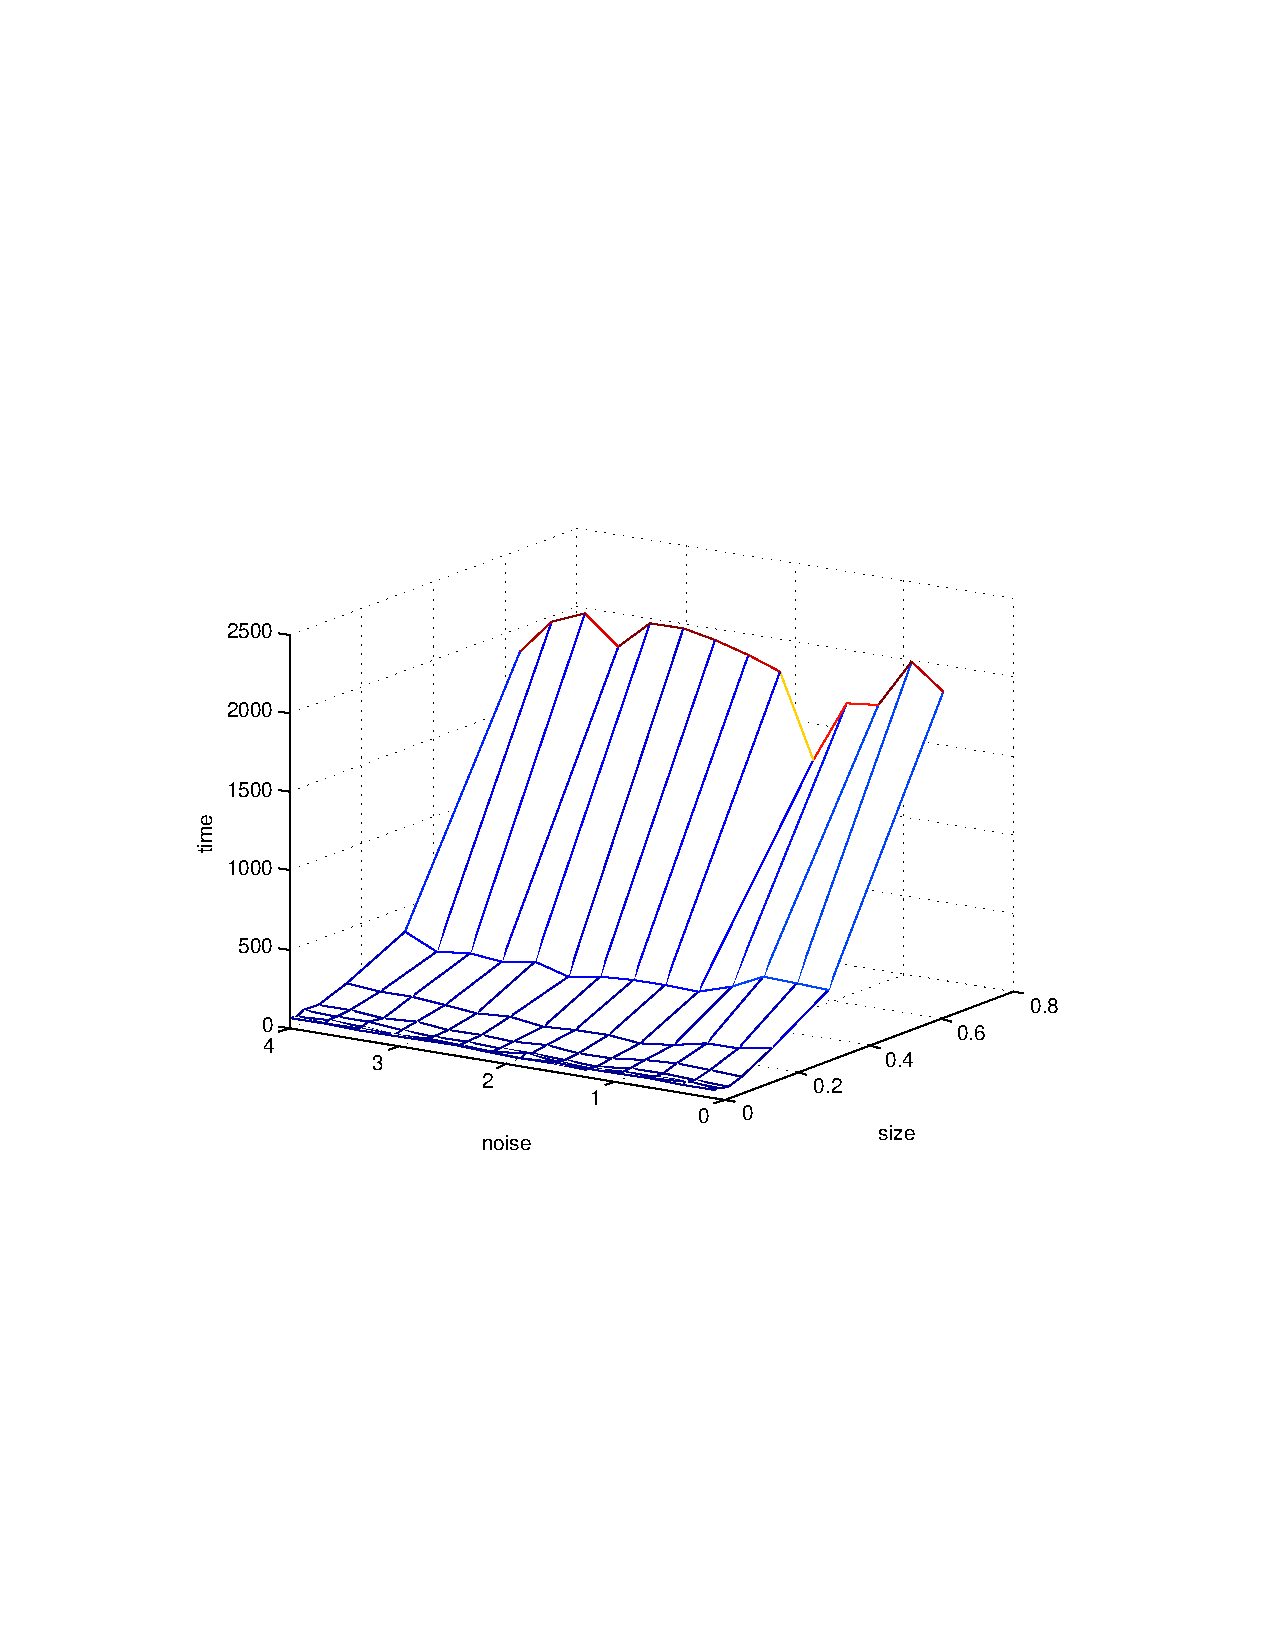
\includegraphics[width=0.45\columnwidth,trim=3.5cm 8cm 4.5cm 8cm,clip]{images/grid-time2.pdf}}
\fbox{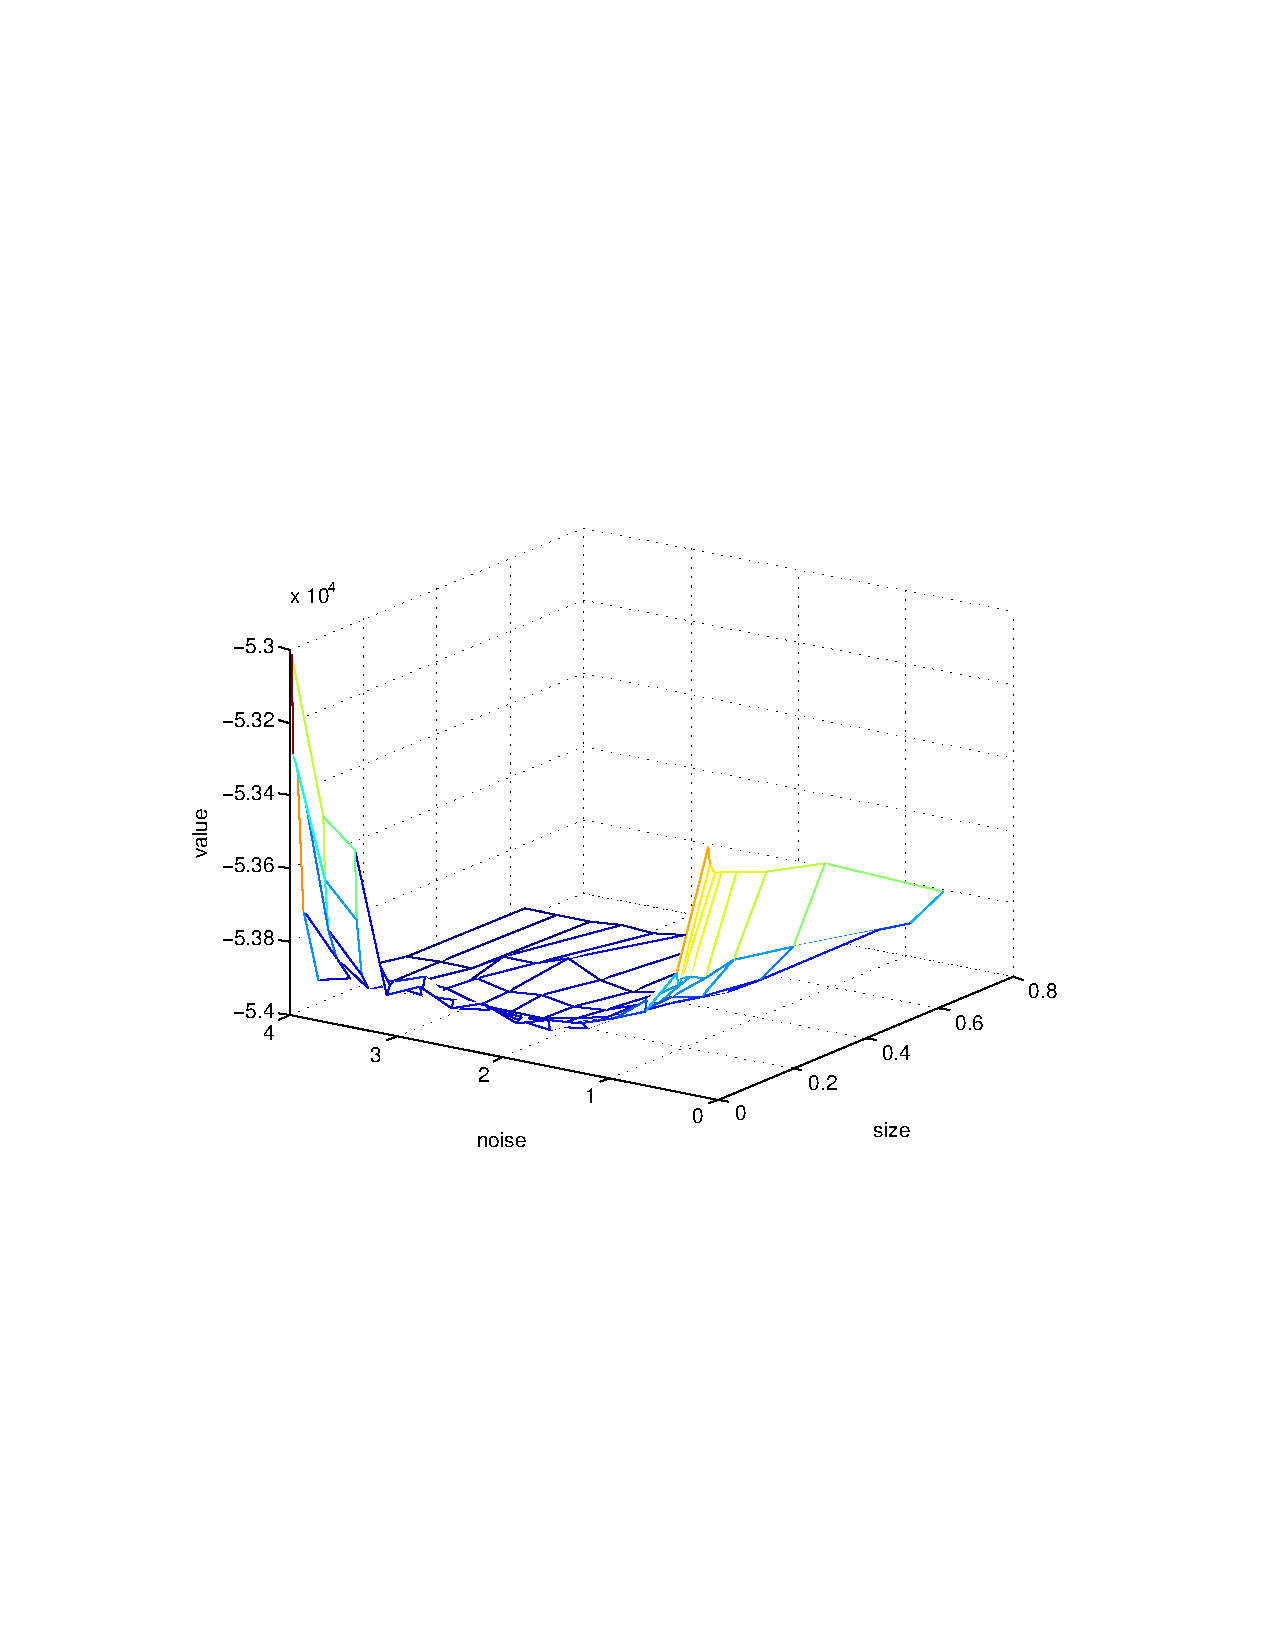
\includegraphics[width=0.45\columnwidth,trim=3.5cm 8cm 4.5cm 8cm,clip]{images/grid-value2.pdf}}
\caption{Empirical evaluation of the impact of noise used for proposal generation and proposal size.
  Proposals with many segments causes longer runtime. Noise seemed not to be a critical parameter but should be selected large enough.
}
\label{fig:parameterchoice}
\end{figure}

\subsection{Social Networks and Network Clustering}\label{sec:nets}
An application for large scale correlation clustering are social networks.
We consider two of those networks from the Stanford Large Network Dataset Collection\footnote{\url{http://snap.stanford.edu/data/index.html}}.
Both networks are given by weighted directed graphs with edge weights $-1$ and $1$. 
%
The first network is called \emph{Epinions}. 
This is who-trust-whom online social network of a a general consumer review site Epinions.com. 
Each directed edge $a\to b$ indicated that user $a$ trusts  or does not trust user $b$ by a  positive or negative edge-weight, respectively.
The network contains $131828$ nodes and $841372$ edges from which $85.3\%$ are positively weighted.
%
The second network is called \emph{Slashdot}. 
Slashdot is a technology-related news website know for its specific user community. 
In 2002 Slashdot introduced the Slashdot Zoo feature which allows users to tag each other as friends or foes. 
The network was obtained in November 2008 and contains $77350$ nodes and $516575$ edges from which $76.73\%$ are positively weighted.

We consider the problem to cluster this graphs such that positively weighted edges ($E^+_{\to}$) link inside and negatively weighted edges ($E^-_{\to}$) between clusters.
In other words friends and people who trust each other should be in the same segment and foes and non-trusting people in different clusters.
% 
To compensate the high impact of nodes with high degree we can normalize the edge weights such that each person has the same impact to the overall network, by enforcing.
\begin{align}
  \sum_{i\to j \in E_{\to}} |w_{i\to j}| &= 1&\forall i\in V, deg^{\textrm{out}}(i)\geq 1 
\end{align}
We define the following energy function
\begin{align}
 J(y) &= \sum_{i\to j \in E^+_{\to}} y_{ij}\cdot w_{i \to j} +  \sum_{i\to j \in E^-_{\to}} (y_{ij}-1)\cdot w_{i \to j} \nonumber\\
      &= \sum_{ij \in E} y_{ij}\cdot \underbrace{(w_{i \to j}+w_{j \to i})}_{w_{ij}} + \textrm{const}
\end{align}
which is zero if the given partitioning does not violated any relation and larger otherwise.
We name this two datasets \emph{social nets} and \emph{normalized social nets}.

As shown in Fig.~\ref{fig:anytime}(g,h) CCFusion provides for the first minutes the best results.
Only CGC and HC-CGC are able to find better solutions after more then 1000 seconds.
MC-I and MC-R can even not be applied on such large problems.
We belief that with better proposal generators, which are more suited for such network problems,
we can improve CCFusion. One candidate for such a generated would be a scalable method for the 
PIVOT algorithm.

As another example for network clustering we use the \emph{modularity-clustering} models from~\cite{kappes_2014_benchmark_arxiv} which are small but fully connected.
Although, CCFusion and the used parameters was not designed and chosen for this type of problem, it performs on par to competitive methods. 
Especially is does a better job than MC-I as shown in Fig.~\ref{fig:anytime}(i)



\subsection{2D and 3D Image Segmentation}\label{sec:imseg}
To segment images or volumes into a previously
unknown number of clusters, correlation clustering
has been used~\cite{andres_2011_iccv,kroeger_2012_eccv}.

Starting from a super-pixel/-voxel segmentation,
correlation clustering finds the clustering with the lowest energy.
The energy is based on a likelihood of merging adjacent super-voxels.
Each edge has a probability to keep adjacent segments separate ($p(y_{ij} =1)$)
or to merge them ($p(y_{ij} = 0)$).
The energy function is defined as following:
\begin{align}
 J(y)  &= \sum_{ij \in E} y_{ij}\cdot \underbrace{  log\left( \frac{p(y_{ij} =0)}{p(y_{ij} =1)}\right) + log \frac{1-\beta}{\beta}  }_{w_{ij}}
\end{align}
Where $\beta$ is used as a prior~\cite{andres_2011_iccv}.

We use the public available benchmark instances from~\cite{kappes_2013_benchmark_cvpr,kappes_2014_benchmark_arxiv}.
For 2D images, we took the segmentation problems on the Berkeley Segmentation Database~\cite{martin_2001} called \emph{image-seg}~\cite{andres_2011_iccv,kappes_2013_benchmark_cvpr}.
For 3D volume segmentation we took the models \emph{knott-3d-150},\emph{-300} and \emph{-450} from~\cite{kroeger_2012_eccv,kappes_2014_benchmark_arxiv} as well as the large
instance from the \emph{3d-seg} model~\cite{andres_2011_iccv,kappes_2013_benchmark_cvpr}. These instances have underling cube sizes of  $150^3$, $300^3$, $450^3$, and $900^3$, respectively.
We also request larger instances from the authors of~\cite{kroeger_2012_eccv} which kindly provide us the dataset~\emph{knott-3d-550} with cube size  $550^3$.
%More information of the size of instances is given in Tab.~\ref{tab:instance_sizes}.

For image-seg CCFusion is faster than competitive methods, \cf Fig.~\ref{fig:anytime}(a).
The variation of information~\cite{} (VI) of the CCFusion methods is also best, \cf Tab.~\ref{tab:eval}.
Proposals by EHC seemed to be a bit better than WS-based ones.

For the knott-datasets similar holds. With increasing problem size CCFusion-HC-MC and CCFusion-WS-MC have a better performance compared to competitive methods, \cf Fig.~\ref{fig:anytime}(b-e).
Also in terms of VI they are only slightly worse than the global optimal solution found by MC-I.
The initialization of CGC by HC denoted by HC-CGC also improves the performance compared to native CGC.
For the largest 3D volume seg-3d, HC-CGC gives the first good solution, \cf  Fig.~\ref{fig:anytime}(f).
However, after a view minutes  CCFusion-HC-MC and CCFusion-WS-MC give much better results and also overall best in terms of energy and VI, \cf Tab.~\ref{tab:eval}.

Pure HC, Fusion and PIVOT-BOEM do not give useful results on any dataset.

\begin{table}[t]
   \tiny
   \centering
   \caption{Evaluation by Variation of Information (VOI) Rand Index (RI) for datasets with available ground-truth.}
   \label{tab:eval}
   \begin{tabular}{lllllll}
      \toprule
         VOI              &  image-seg   & knott-3d-150 & knott-3d-300   & knott-3d-450 & knott-3d-550 &3d-seg\\
      \midrule 
         PIVOT-BOEM       &\rd$ 4.9633$  &\rd $ 2.9936$ &\rd $ 4.4986$   &      --      &    --        &  --\\ 
         HC               &   $ 2.5967$  &    $ 1.5477$ &    $ 2.3513$   &    $ 2.9155$ &    --        & $       2.8395$\\
         HC-CGC           &   $ 2.5164$  &    $ 0.9052$ &    $ 1.7636$   &    $ 2.2256$ &    --        & $       1.7603$ \\
         CGC              &   $ 2.5247$  &    $ 0.9267$ &    $ 1.8822$   &    $ 2.3104$ &    --        & $\rd    6.8908$ \\
         KL               &   $ 2.6432$  &\rd $ 2.0648$ &\rd $ 4.1318$   &\rd $ 4.9270$ &    --        & $\rd    7.1057$\\
         FUSION           &$\bf 2.1406$  &\rd $ 2.8787$ &\rd $ 4.0744$   &\rd $ 4.6616$ &    --        & $\rd    6.5366$ \\
         MC-R             &   $ 2.5471$  &    $ 0.9178$ &    $ 1.6369$   &    $ 2.8710$ &    --        & $\rd    6.5058$\\   
         MC-I             &   $ 2.5367$  & $\bf 0.9063$ & $\bf 1.6352$   & $\bf 2.0037$ &    --        & $\rd    4.3319$\\  
         FusionCC-HC-MC   &   $ 2.5319$  &    $ 0.9629$ &    $ 1.6516$   &    $ 2.0801$ &    --        & $\bf    1.3347$ \\  
         FusionCC-HC-CGC  &$\bf 2.4961$  &    $ 0.9679$ &    $ 1.7673$   &    $ 2.3809$ &    --        & $       2.1347$ \\  
         FusionCC-WS-MC   &   $ 2.5340$  &    $ 0.9629$ &    $ 1.6742$   &    $ 2.0739$ &    --        & $\bf    1.3334$ \\  
         FusionCC-WS-CGC  &   $ 2.5192$  &    $ 1.0585$ &    $ 2.1344$   &    $ 2.7487$ &    --        & $       3.3514$ \\      
      \bottomrule
   \end{tabular}

   \begin{tabular}{lllllll}
      \toprule
          RI              &  image-seg   & knott-3d-150 & knott-3d-300   & knott-3d-450 & knott-3d-550 &3d-seg\\
      \midrule 
         PIVOT-BOEM       &   $ 0.7438$  &\rd $ 0.7851$ &    $  0.8792$  &      --      &    --        &  --\\ 
         HC               &   $ 0.7560$  &\rd $ 0.8139$ &\rd $  0.8084$  &\rd $ 0.7610$ &    --        &   $ 0.9651$\\
         HC-CGC           &   $ 0.7724$  &    $ 0.9226$ &    $  0.8713$  &    $ 0.8433$ &    --        &   $ 0.9861$ \\
         CGC              &   $ 0.7590$  &    $ 0.9206$ &    $  0.8666$  &    $ 0.8341$ &    --        &\rd$ 0.6024$ \\
         KL               &\rd$ 0.6400$  &\rd $ 0.8085$ &\rd $  0.6858$  &\rd $ 0.6409$ &    --        &\rd$ 0.5849$\\
         FUSION           &\rd$ 0.5480$  &\rd $ 0.2849$ &\rd $  0.1420$  &\rd $ 0.0998$ &    --        &\rd$ 0.0345$ \\
         MC-R             &   $ 0.7822$  &    $ 0.9232$ & $\bf  0.8849$  &\rd $ 0.6713$ &    --        &\rd$ 0.0432$ \\   
         MC-I             &   $ 0.7821$  & $\bf 0.9236$ & $\bf  0.8849$  & $\bf 0.8670$ &    --        &\rd$ 0.5461$\\  
         FusionCC-HC-MC   &   $ 0.7801$  &    $ 0.9042$ &    $  0.8824$  &    $ 0.8573$ &    --        &$\bf 0.9906$ \\  
         FusionCC-HC-CGC  &   $ 0.7780$  &    $ 0.9031$ &    $  0.8763$  &    $ 0.8470$ &    --        &   $ 0.9775$ \\  
         FusionCC-WS-MC   &$\bf 0.7825$  &    $ 0.9042$ &    $  0.8802$  &    $ 0.8582$ &    --        &   $ 0.8895$ \\  
         FusionCC-WS-CGC  &   $ 0.7750$  &    $ 0.8951$ &    $  0.8596$  &    $ 0.8394$ &    --        &   $\bf 0.9906$ \\      
      \bottomrule
   \end{tabular}
\end{table}

%\begin{center}
%    \begin{figure}
%        \begin{center}
%            \begin{subfigure}[b]{0.45\linewidth}
%                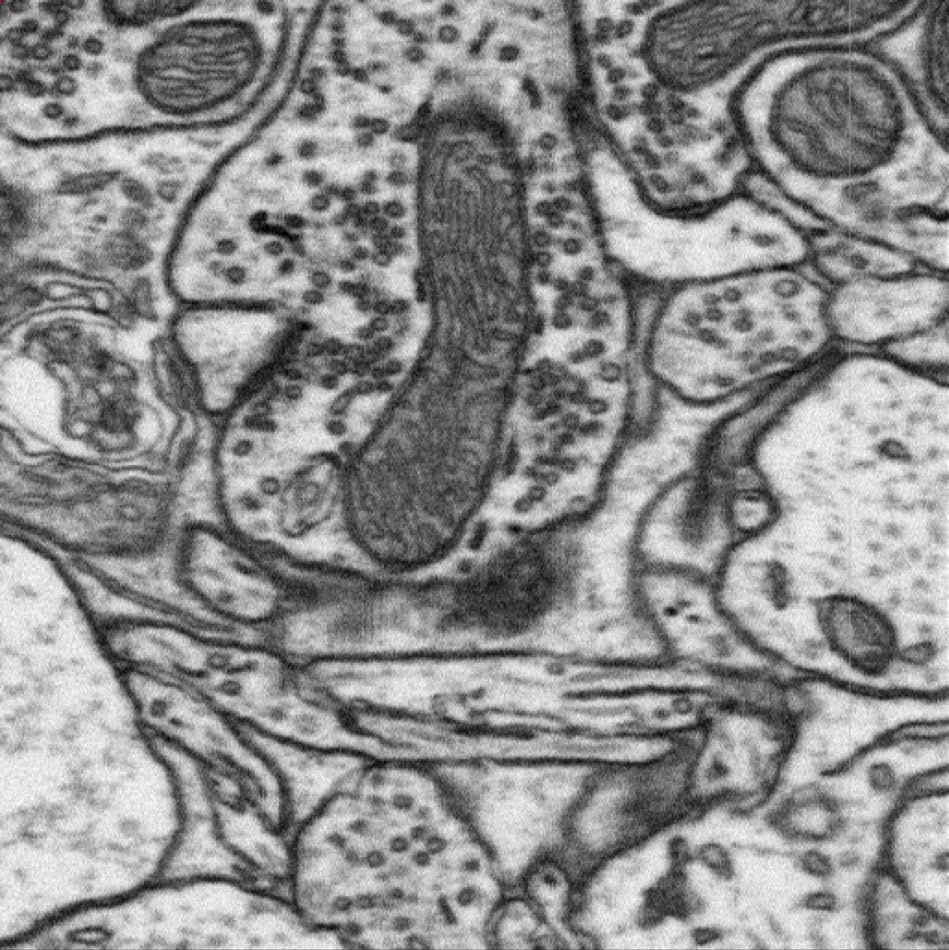
\includegraphics[width=1.0\linewidth]{images/-010.jpg}
%            \end{subfigure}
%            \quad
%            \begin{subfigure}[b]{0.45\linewidth}
%                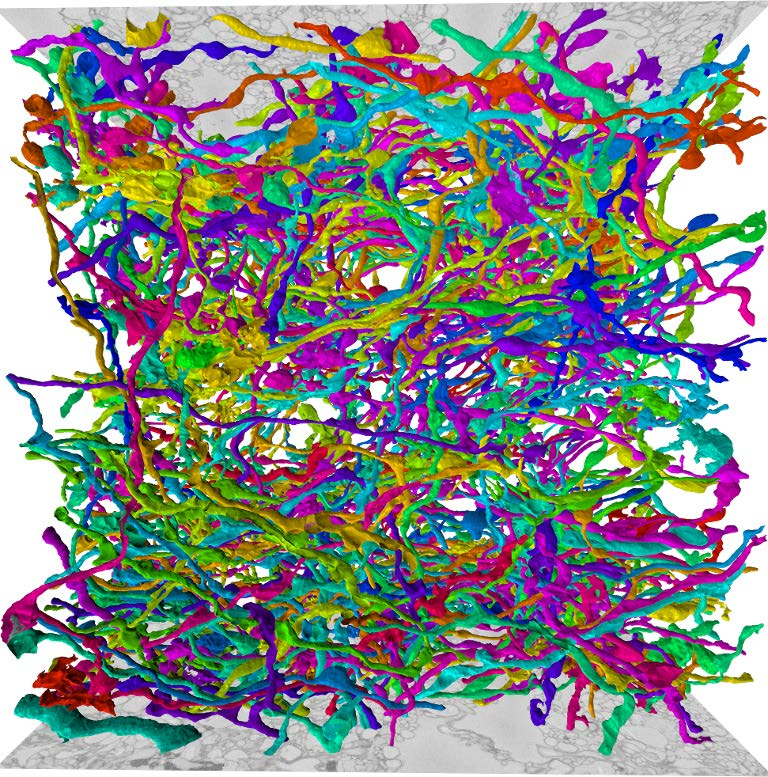
\includegraphics[width=1.0\linewidth]{images/-030.jpg}
%            \end{subfigure}
%        \end{center}
%    \caption{
%        Raw FIBSEM data and correlation clustering result of the model from \cite{kroeger_2012_eccv%}
%    }
%    \end{figure}
%\end{center}
%
%\newpage



%!TEX root = egpaper_for_review.tex
%%%%%%%%%%%%%%%%%%%%%%%%%%%%%%%%%%%%%%%%%%%%%%%%%%%%%%%%%%%%%%%%%%%%%%%%%%%%%%%%%%%%%%%%%%%%
\pgfplotsset{every axis legend/.append style={
at={(1.0,1.2)},
anchor=north east}} 
\begin{figure*}[p]
  \begin{subfigure}[b]{0.33\textwidth}
  \centering
  \begin{tikzpicture}
  \begin{semilogxaxis}[  mark size=1pt,
  restrict y to domain=0:4620,
  xlabel = {runtime},
  xmin = 0,
  xmax = 4100,
  width = 1.0\columnwidth,
  scaled ticks = false,
  every axis legend/.code={\let\addlegendentry\relax} 
  ]  
  \anytimeplot{image-seg}
  \end{semilogxaxis}
  \end{tikzpicture}
  \caption{image-seg}\label{fig:at:image-seg}
  \end{subfigure}
  %%%%%%%%%%%%%%%%%%%%%%%%%%%%%%%%%%%%%%%%%%%%%%%%%%%%%%%%%%%%%%%%%%%%%%%%% 
  \begin{subfigure}[b]{0.33\textwidth}
    \centering
    \begin{tikzpicture}
    \begin{semilogxaxis}[  mark size=1pt,
   % restrict y to domain=-6000:-4400,
    xlabel = {runtime},
    xmin = 0,
    xmax = 4100,
    width = 1.0\columnwidth,
    scaled ticks = false,
    every axis legend/.code={\let\addlegendentry\relax} 
    ] 
    \anytimeplot{knott-3d-150}
    \addplot[color=yellow,mark=square] table[x=time,y=PIVOT*]{data3/knott-3d-150.data};  
   
    \end{semilogxaxis}
    \end{tikzpicture}
    \caption{knott-3d-150}\label{fig:at:knott-150}
  \end{subfigure}
  %%%%%%%%%%%%%%%%%%%%%%%%%%%%%%%%%%%%%%%%%%%%%%%%%%%%%%%%%%%%%%%%%%%%%%%%%%%%%%%%%%%%%%%%%%%%%
  \begin{subfigure}[b]{0.33\textwidth}
  \centering
  \begin{tikzpicture}
  \begin{semilogxaxis}[  mark size=1pt,
  restrict y to domain=-40000:-24000,
  xlabel = {runtime},
  xmin = 0,
  xmax = 4100,
  width = 1.0\columnwidth,
  scaled ticks = false,
  legend to name = ledgendPosition,
  legend columns=6
  ]  
  \anytimeplot{knott-3d-300}
  \end{semilogxaxis}
  \end{tikzpicture}
  \caption{knott-3d-300}\label{fig:at:knott-300}
  \end{subfigure}
  \newline
  %%%%%%%%%%%%%%%%%%%%%%%%%%%%%%%%%%%%%%%%%%%%%%%%%%%%%%%%%%%%%%%%%%%%%%%%%%%%%%%%%%%%%%%%%%%%%
  \begin{subfigure}[b]{0.33\textwidth}
  \centering
  \begin{tikzpicture}
  \begin{semilogxaxis}[  mark size=1pt,
  restrict y to domain=-80000:-60000,
  xlabel = {runtime},
  xmin = 0,
  xmax = 4100,
  width = 1.0\columnwidth,
  scaled ticks = false,
  every axis legend/.code={\let\addlegendentry\relax} 
  ] 
  \anytimeplot{knott-3d-450} 
  \end{semilogxaxis}
  \end{tikzpicture}
  \caption{knott-3d-450}\label{fig:at:knott-450}
  \end{subfigure}
  %%%%%%%%%%%%%%%%%%%%%%%%%%%%%%%%%%%%%%%%%%%%%%%%%%%%%%%%%%%%%%%%%%%%%%%%%%%%%%%%%%%%%%%%%%%%%
  \begin{subfigure}[b]{0.33\textwidth}
  \centering
  \begin{tikzpicture}
  \begin{semilogxaxis}[  mark size=1pt,
  restrict y to domain=-10000000:-100000,
  xlabel = {runtime},
  xmin = 0,
  xmax = 4100,
  width = 1.0\columnwidth,
  scaled ticks = false,
  every axis legend/.code={\let\addlegendentry\relax} 
  ]
  \anytimeplot{knott-3d-550} 
  \end{semilogxaxis}
  \end{tikzpicture}
  \caption{knott-3d-550}\label{fig:at:knott-550}
  \end{subfigure}
  %%%%%%%%%%%%%%%%%%%%%%%%%%%%%%%%%%%%%%%%%%%%%%%%%%%%%%%%%%%%%%%%%%%%%%%%%%%%%%%%%%%%%%%%%%%%%\begin{subfigure}[H]
  \begin{subfigure}[b]{0.33\textwidth}
  \centering
  \begin{tikzpicture}
  \begin{semilogxaxis}[  mark size=1pt,
  %restrict y to domain=-10000000:-100000,
  %restrict y to domain=-10000000:1200000,
  xlabel = {runtime},
  xmin = 0,
  xmax = 4100,
  width = 1.0\columnwidth,
  scaled ticks = false,
  every axis legend/.code={\let\addlegendentry\relax} 
  ] 
  \anytimeplot{seg-3d} 
  \end{semilogxaxis}
  \end{tikzpicture}
  \caption{seg-3d}\label{fig:at:seg3d}
  \end{subfigure}
 %%%%%%%%%%%%%%%%%%%%%%%%%%%%%%%%%%%%%%%%%%%%%%%%%%%%%%%%%%%%%%%%%%%%%%%%%%%%%%%%%%%%%%%%%%%%%
  \begin{subfigure}[b]{0.33\textwidth}
  \centering
  \begin{tikzpicture}
  \begin{semilogxaxis}[  mark size=1pt,
  %restrict y to domain=-10000000:-100000,
  %restrict y to domain=-10000000:100000,
  xlabel = {runtime},
  xmin = 0,
  xmax = 4100,
  width = 1.0\columnwidth,
  scaled ticks = false,
  every axis legend/.code={\let\addlegendentry\relax} 
  ]  
  \addplot[color=brown,mark=x] table[x=time,y=HC]{data3/socialnets.data};              \addlegendentry{HC}
  \addplot[color=black,mark=square] table[x=time,y=HC-CGC]{data3/socialnets.data};          \addlegendentry{HC-CGC}
  \addplot[color=red,mark=x] table[x=time,y=CGC]{data3/socialnets.data};               \addlegendentry{CGC}
  %\addplot[color=gray,mark=o] table[x=time, y=ogm-KL]{data3/normalizedsocialnets.data};          \addlegendentry{KL}
  \addplot[color=purple,mark=o] table[x=time, y=MCR-CCFDB]{data3/socialnets.data};     \addlegendentry{MC-R}
  \addplot[color=blue,mark=o] table[x=time, y=MCI-CCIFD]{data3/socialnets.data};       \addlegendentry{MC-I}
  \addplot[color=green,mark=o] table[x=time, y=DYNCC-HC-MC]{data3/socialnets.data};    \addlegendentry{Fusion-HC-MC}
  \addplot[color=cyan,mark=x] table[x=time, y=DYNCC-HC-CGC]{data3/socialnets.data};    \addlegendentry{Fusion-HC-CGC}
  %\addplot[color=orange,mark=o] table[x=time, y=DYNCC-WS-MC]{data3/normalizedsocialnets.data};  \addlegendentry{Fusion-WS-MC}
  \addplot[color=pink,mark=x] table[x=time, y=DYNCC-WS-CGC]{data3/socialnets.data};  \addlegendentry{Fusion-WS-CGC}
  %\anytimeplot{socialnets} 
  \end{semilogxaxis}
  \end{tikzpicture}
  \caption{social nets}\label{fig:at:socialnets}
  \end{subfigure}
 %%%%%%%%%%%%%%%%%%%%%%%%%%%%%%%%%%%%%%%%%%%%%%%%%%%%%%%%%%%%%%%%%%%%%%%%%%%%%%%%%%%%%%%%%%%%%
  \begin{subfigure}[b]{0.33\textwidth}
  \centering
  \begin{tikzpicture}
  \begin{semilogxaxis}[  mark size=1pt,
  %restrict y to domain=-10000000:-100000,
  %restrict y to domain=-10000000:100000,
  xlabel = {runtime},
  xmin = 0,
  xmax = 4100,
  width = 1.0\columnwidth,
  scaled ticks = false,
  every axis legend/.code={\let\addlegendentry\relax} 
  ] 
  \addplot[color=brown,mark=x] table[x=time,y=HC]{data3/normalizedsocialnets.data};              \addlegendentry{HC}
  %\addplot[color=black,mark=square] table[x=time,y=HC-CGC]{data3/normalizedsocialnets.data};          \addlegendentry{HC-CGC}
  \addplot[color=red,mark=x] table[x=time,y=CGC]{data3/normalizedsocialnets.data};               \addlegendentry{CGC}
  %\addplot[color=gray,mark=o] table[x=time, y=ogm-KL]{data3/normalizedsocialnets.data};          \addlegendentry{KL}
  \addplot[color=purple,mark=o] table[x=time, y=MCR-CCFDB]{data3/normalizedsocialnets.data};     \addlegendentry{MC-R}
  \addplot[color=blue,mark=o] table[x=time, y=MCI-CCIFD]{data3/normalizedsocialnets.data};       \addlegendentry{MC-I}
  \addplot[color=green,mark=o] table[x=time, y=DYNCC-HC-MC]{data3/normalizedsocialnets.data};    \addlegendentry{Fusion-HC-MC}
  \addplot[color=cyan,mark=x] table[x=time, y=DYNCC-HC-CGC]{data3/normalizedsocialnets.data};    \addlegendentry{Fusion-HC-CGC}
  %\addplot[color=orange,mark=o] table[x=time, y=DYNCC-WS-MC]{data3/normalizedsocialnets.data};  \addlegendentry{Fusion-WS-MC}
  \addplot[color=pink,mark=x] table[x=time, y=DYNCC-WS-CGC]{data3/normalizedsocialnets.data};  \addlegendentry{Fusion-WS-CGC}
 % \anytimeplot{normalizedsocialnets}
  \end{semilogxaxis}
  \end{tikzpicture}
  \caption{normalized social nets}\label{fig:at:nsocialnets}
  \end{subfigure}
 %%%%%%%%%%%%%%%%%%%%%%%%%%%%%%%%%%%%%%%%%%%%%%%%%%%%%%%%%%%%%%%%%%%%%%%%%%%%%%%%%%%%%%%%%%%%%
  \begin{subfigure}[b]{0.33\textwidth}
  \centering
  \begin{tikzpicture}
  \begin{semilogxaxis}[  mark size=1pt,
  %restrict y to domain=-10000000:-100000,
  %restrict y to domain=-10000000:100000,
  xlabel = {runtime},
  xmin = 0,
  xmax = 4100,
  width = 1.0\columnwidth,
  scaled ticks = false,
  every axis legend/.code={\let\addlegendentry\relax} 
  ] 
  \anytimeplot{modularity-clustering}
    \addplot[color=yellow,mark=square] table[x=time,y=PIVOT*]{data3/modularity-clustering.data};
  \end{semilogxaxis}
  \end{tikzpicture}
  \caption{modularity clustering}\label{fig:at:modularity}
  \end{subfigure}
 %%%%%%%%%%%%%%%%%%%%%%%%%%%%%%%%%%%%%%%%%%%%%%%%%%%%%%%%%%%%%%%%%%%%%%%%%%%%%%%%%%%%%%%%%%%%%

  \begin{center}
  \hypersetup{linkcolor = black}
  \ref{ledgendPosition}
  \hypersetup{linkcolor = red}
  \end{center}
  \caption{
    % image seg
    For the image-seg instances in fig.~\ref{fig:at:image-seg} 
    Fusion-EHC-MC has performs best and Fusion-WS-MC gives 
    almost the same results, but a bit slower then with EHC proposals.
    Using the same proposals but approximate moves (Fusion-EHC-CGC Fusion-WS-CGC )
    leads to suboptimal results.
    The warm EHC started version of GCG (EHC-CGC) performs better then GCG itself,
    but both are outperformed by the proposed algorithms.
    Global optimal methods (MC-I) and the relaxed version (MC-R) are 
    still usable fast for these instances.
    % 3d 
    For the smallest 3D instances (\ref{fig:at:knott-150}) all solvers
    except ??? and EHC perform equally, and the proposed fusion algorithms
    give the best any time performance.
    With increasing problem size (\ref{fig:at:knott-150}-\ref{fig:at:knott-550} and \ref{fig:at:seg3d})
    the runtime of MC-I, MC-R and CGC increases drastically, while
    the proposed solvers still scale well.
    For these instances, the EHC started version of CGC outperforms 
    GCG in terms of runtime and energy.
    % social nets
    For the social net instances (\ref{fig:at:socialnets},\ref{fig:at:nsocialnets})
    Fusion-HC-MC and Fusion-HC-CGC perform equally.
    Only CGC and EHC-CGC leads to better energies after $10^3 sec$, while global optimal methods (MC-I)
    fail to converge within this time limit.
    % modularity clustering 
    For the modularity clustering instances in fig.~\ref{fig:at:modularity} we see
    an interesting behavior. On these complete graphs, Kernighan Lin (KL) has the 
    best performance.
    The proposed methods perform reasonable, but  KL is faster and leads to better energies.
    %%%
    %% summary
    Overall, energy hierarchical clustering based proposals work better
    then watershed based proposals. They converge to similar energies
    but the clustering based approach is faster on all tested instances.
    On all instances except for modularity clustering, it is better
    to solve the fusion move to optimality (Fusion-HC-MC) then using approximations (FUSION-HC-GCG).
  }
\end{figure*}
%%%%%%%%%%%%%%%%%%%%%%%%%%%%%%%%%%%%%%%%%%%%%%%%%%%%%%%%%%%%%%%%%%%%%%%%%%%%%%%%%%%%%%%%%%%%%





% \begin{figure}
% \begin{tikzpicture}
  \begin{loglogaxis}[
    xlabel = {runtime},
    ylabel = {distance to optimum/best},
    xlabel style={name=xlabel},
    mark size=1pt,
    every axis/.append style={font=\tiny}, 
    width = 0.95\columnwidth, 
    height= 0.95\columnwidth, 
    legend style = { at={(xlabel.south)}, yshift=-1ex, anchor=north,legend cell align=left, font=\tiny},  
    legend columns = 4 
   ]
  \addplot[only marks, mark=*,red, line width=\thickline,opacity=0.8] table[x=Togm_CGC, y=Vogm_CGC]{\scatterplotpath knott-3d-450.data}; 
  \addlegendentry{CGC};   
 % \addplot[only marks, mark=*,green, line width=\thickline,opacity=0.8] table[x=Togm_HC, y=Vogm_HC]{\scatterplotpath knott-3d-450.data}; 
  %\addlegendentry{HC};   
  \addplot[only marks, mark=*,orange!50, line width=\thickline,opacity=0.8] table[x=Togm_HC_CGC, y=Vogm_HC_CGC]{\scatterplotpath knott-3d-450.data}; 
  \addlegendentry{HC-CGC};   
  %\addplot[only marks, mark=*,cyan, line width=\thickline,opacity=0.8] table[x=Togm_icm, y=Vogm_icm]{\scatterplotpath knott-3d-450.data}; 
  %\addlegendentry{ogm-ICM};   
  \addplot[only marks, mark=*,magenta, line width=\thickline,opacity=0.8] table[x=Togm_kl, y=Vogm_kl]{\scatterplotpath knott-3d-450.data}; 
  \addlegendentry{ogm-KL};   
  %\addplot[only marks, mark=*,black, line width=\thickline,opacity=0.8] table[x=Togm_lf1, y=Vogm_lf1]{\scatterplotpath knott-3d-450.data}; 
  %\addlegendentry{ogm-LF-1};   
  %\addplot[only marks, mark=*,brown, line width=\thickline,opacity=0.8] table[x=Togm_mcfusion_HC_BASE, y=Vogm_mcfusion_HC_BASE]{\scatterplotpath knott-3d-450.data}; 
  %\addlegendentry{DYNCC-HC-B};   
  %\addplot[only marks, mark=*,yellow!70!black, line width=\thickline,opacity=0.8] table[x=Togm_mcfusion_HC_BASE_CGCF, y=Vogm_mcfusion_HC_BASE_CGCF]{\scatterplotpath knott-3d-450.data}; 
  %\addlegendentry{DYNCC-HC-B-CGC};   
  %\addplot[only marks, mark=*,blue!40, line width=\thickline,opacity=0.8] table[x=Togm_mcfusion_HC_CGC, y=Vogm_mcfusion_HC_CGC]{\scatterplotpath knott-3d-450.data}; 
  %\addlegendentry{DYNCC-HC-CGC};   
  \addplot[only marks, mark=*,blue, line width=\thickline,opacity=0.8] table[x=Togm_mcfusion_HC_CGC_CGCF, y=Vogm_mcfusion_HC_CGC_CGCF]{\scatterplotpath knott-3d-450.data}; 
  \addlegendentry{DYNCC-HC-CGC-CGC};   
  %\addplot[only marks, mark=x,red, line width=\thickline,opacity=0.8] table[x=Togm_mcfusion_HC_MC, y=Vogm_mcfusion_HC_MC]{\scatterplotpath knott-3d-450.data}; 
  %\addlegendentry{DYNCC-HC-MC};   
  \addplot[only marks, mark=x,green, line width=\thickline,opacity=0.8] table[x=Togm_mcfusion_HC_MC_CGCF, y=Vogm_mcfusion_HC_MC_CGCF]{\scatterplotpath knott-3d-450.data}; 
  \addlegendentry{DYNCC-HC-MC-CGC};   
  %\addplot[only marks, mark=x,orange!50, line width=\thickline,opacity=0.8] table[x=Togm_mcfusion_WS_BASE, y=Vogm_mcfusion_WS_BASE]{\scatterplotpath knott-3d-450.data}; 
  %\addlegendentry{DYNCC-WS-B};   
  %\addplot[only marks, mark=x,cyan, line width=\thickline,opacity=0.8] table[x=Togm_mcfusion_WS_BASE_CGCF, y=Vogm_mcfusion_WS_BASE_CGCF]{\scatterplotpath knott-3d-450.data}; 
  %\addlegendentry{DYNCC-WS-B-CGC};   
  %\addplot[only marks, mark=x,magenta, line width=\thickline,opacity=0.8] table[x=Togm_mcfusion_WS_CGC, y=Vogm_mcfusion_WS_CGC]{\scatterplotpath knott-3d-450.data}; 
  %\addlegendentry{DYNCC-WS-CGC};   
  %\addplot[only marks, mark=x,black, line width=\thickline,opacity=0.8] table[x=Togm_mcfusion_WS_CGC_CGCF, y=Vogm_mcfusion_WS_CGC_CGCF]{\scatterplotpath knott-3d-450.data}; 
  %\addlegendentry{DYNCC-WS-CGC-CGC};   
  %\addplot[only marks, mark=x,brown, line width=\thickline,opacity=0.8] table[x=Togm_mcfusion_WS_MC, y=Vogm_mcfusion_WS_MC]{\scatterplotpath knott-3d-450.data}; 
  %\addlegendentry{DYNCC-WS-MC};   
  %\addplot[only marks, mark=x,yellow!70!black, line width=\thickline,opacity=0.8] table[x=Togm_mcfusion_WS_MC_CGCF, y=Vogm_mcfusion_WS_MC_CGCF]{\scatterplotpath knott-3d-450.data}; 
  %\addlegendentry{DYNCC-WS-MC-CGC};   
  \addplot[only marks, mark=x,blue!40, line width=\thickline,opacity=0.8] table[x=TMC_CC, y=VMC_CC]{\scatterplotpath knott-3d-450.data}; 
  \addlegendentry{MCR-CC};   
  %\addplot[only marks, mark=x,blue, line width=\thickline,opacity=0.8] table[x=TMC_CCFDB, y=VMC_CCFDB]{\scatterplotpath knott-3d-450.data}; 
  %\addlegendentry{MCR-CCFDB};   
  %\addplot[only marks, mark=square*,red, line width=\thickline,opacity=0.8] table[x=TMC_CCFDB_OWC, y=VMC_CCFDB_OWC]{\scatterplotpath knott-3d-450.data}; 
  %\addlegendentry{MCR-CCFDB-OWC};   
  %\addplot[only marks, mark=square*,green, line width=\thickline,opacity=0.8] table[x=TMC_CCFDB_CCIFD, y=VMC_CCFDB_CCIFD]{\scatterplotpath knott-3d-450.data}; 
  %\addlegendentry{MCI-CCFDB-CCIFD};   
  \addplot[only marks, mark=square*,orange!50, line width=\thickline,opacity=0.8] table[x=TMC_CCI, y=VMC_CCI]{\scatterplotpath knott-3d-450.data}; 
  \addlegendentry{MCI-CCI};   
  \addplot[only marks, mark=square*,cyan, line width=\thickline,opacity=0.8] table[x=TMC_CCIFD, y=VMC_CCIFD]{\scatterplotpath knott-3d-450.data}; 
  \addlegendentry{MCI-CCIFD};   
  \end{loglogaxis} 
\end{tikzpicture} 

% \caption{Values and runtime for the 8 knott-3d-450 instances. Note that we use for DYNCC a defensive stopping condition.
% A more aggressive one would lead to much faster runtime with only a bit worse values.
% DYNCC find solutions with less than distance 100 to the optimum a magnitude faster than the state of the art, which produce poor results on hard instances with a 1 hour time limit.
% }
% \end{figure}



%\subsection{Pixel-wise Multicuts}
%%!TEX root = ../egpaper_for_review.tex

\newcounter{cX}
\newcounter{cY}


\newcounter{NPY}
\setcounter{NPY}{30}
\tikzstyle{pixel}=[opacity=1.0,thick,draw opacity=1.0, draw=black]
\tikzstyle{ln}=[opacity=0.6,fill=green,circle,draw, inner sep=0,font=\tiny,minimum size=0.15cm]
\tikzstyle{gn}=[opacity=0.6,fill=red,circle,draw, inner sep=0,font=\tiny,minimum size=0.15cm]
\tikzstyle{p}=[opacity=0.6,fill=white,circle,draw, inner sep=0,font=\tiny,minimum size=0.15cm]
\begin{figure}
\begin{center}
\begin{tikzpicture}[scale=1.0]
    \node[anchor=south west,inner sep=0] (image) at (0,0) 
        {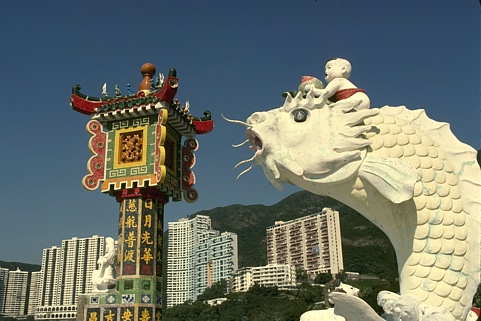
\includegraphics[width=0.4\textwidth]{images/120093.jpg}};
    % shift scope to the image 
    \begin{scope}[x={(image.south east)},y={(image.north west)},xscale=100/481,yscale=100/321]   
        \draw[gray,xstep=3.21/\theNPY, ystep=3.21/\theNPY] (0,0) grid (4.81,3.21);
        % scope of the grid
        \begin{scope}[xscale=3.21/\theNPY,yscale=3.21/\theNPY]  

        \foreach \x\y in {22/18, 10/8} { 
        \setcounter{cX}{\x}
        \setcounter{cY}{\y}
        \draw (\thecX+0.5,\thecY+0.5) node[p]  (centerPixel){};
        \foreach \xx in {-4,0,4} { 
        \foreach \yy in {-4,0,4} { 
            \ifthenelse{\NOT 0 = \xx \OR \NOT 0 = \yy}{
                %\filldraw[green!40!white,pixel] 
                %(\thecX+\xx,\thecY+\yy) rectangle (\thecX+1+\xx,\thecY+1+\yy);
                \draw (\thecX+\xx+0.5,\thecY+\yy+0.5) node[gn](nonLocalPixel){};
                \path[]
                (centerPixel) edge[bend left=0*\xx*\yy ] (nonLocalPixel)
                ;
            }{
            }
        }
        }
        \foreach \xx/\yy/\pColor in {0/1/blue, 0/-1/blue, 1/0/blue, -1/0/blue} { 
            \draw (\thecX+\xx+0.5,\thecY+\yy+0.5) node[ln](nonLocalPixel){};
            (\thecX+\xx,\thecY+\yy) rectangle (\thecX+1+\xx,\thecY+1+\yy);
        }
        }
        % \filldraw[gray,pixel] (\thecX,\thecY) rectangle (\thecX+1,\thecY+1);
        

        \end{scope}
    \end{scope}


\end{tikzpicture}
\end{center}
\caption{
    Pixel Level Multicut:
    every pixel (white nodes) is connected
    to its 4 \emph{local} neighbors (edges between white and green nodes).
    Furthermore each pixel is connected to some \emph{non-local} neighbors within a 
    certain radius  (edges between white and green nodes).
    The local neighbors are connected with a \emph{positive}
    edge weight. If the edge indicator (as gradient magnitude)
    is very high, the local edge weight should be close to zero.
    If there is no evidence for a cut (low gradient magnitude for example)
    the local edge weight should be high.
    The \emph{non-local edge weights} are \emph{negative} to
    encourage label transitions.
    The weight of the non-local edge weights can
    be the negative value of the maximum gradient magnitude
    along a line between the red and white node.
    If there is evidence for a cut between red and white, 
    the weight should be strongly(?) negative.
}
\end{figure}







\section{Future Work}\label{sec:future}
In future work we would like to investigate in much larger problem instances
and interactive correlation clustering, by enforcing
updates only in local regions by appropriate proposals.
%
Within this challenging task we can also enforce additionally must-not-link constraints in eq.~\ref{eq:fusion_move_a}.
If those build a closed surface, the problem decompose into two independent problems.
%
Overall, a more specific selection of proposals, maybe conditioned on the current solution,
should lead better proposals and to faster progress of CCFusion.
%
Furthermore, we can extend our approach to higher-order correlation clustering~\cite{Kim-2011,kappes_2013_arxiv}
by using higher order subproblems.


\section{Conclusion}\label{sec:conclusion}

We have presented a fast and scalable 
approximate solver for correlation 
clustering, named Correlation Clustering Fusion (CCFusion).
It is orthogonal to previous research, \ie it can be combined with and
correlation clustering solver.
%
The best solution is iteratively improved 
by a fusion with proposal solutions.
The fusion move itself is formulated as correlation
clustering on a smaller graph fewer edges and nodes
and can therefore be solved much faster than the original problem.

Our evaluation shows that several CCFusion
outperforms state-of-the-art solvers w.r.t. any time performance 
with increasing problem size.


    


\newpage

\FloatBarrier
{\small
\bibliographystyle{ieee}
\bibliography{egbib}
}

% \newpage

% \onecolumn
% \section{Appendix}

% \begin{table}[H]
\scriptsize
\centering
\caption{image-seg (100 instances)}
\label{tab:smalltable-image-seg}
\begin{tabular}{lrrrrrr}
\toprule
           algorithm &       runtime     &         value &         bound &           mem &     best &      opt   \\ \midrule 
     ogm-CGC-planar* & $         0.28$ sec & $      4445.22$ & $      4136.83$ & $         0.02$ GB & $      28$ & $       0$ \\ 
ogm-mcfusion-HC-BASE* & $         0.12$ sec & $      5462.60$ & $-\infty$ & $         0.01$ GB & $       0$ & $       0$ \\ 
ogm-mcfusion-HC-BASE-CGCF* & $         0.12$ sec & $      5085.80$ & $-\infty$ & $         0.01$ GB & $       0$ & $       0$ \\ 
ogm-mcfusion-HC-CGC* & $         1.23$ sec & $      4444.56$ & $-\infty$ & $         0.01$ GB & $      40$ & $       0$ \\ 
ogm-mcfusion-HC-CGC-CGCF* & $         1.22$ sec & $      4444.75$ & $-\infty$ & $         0.02$ GB & $      40$ & $       0$ \\ 
 ogm-mcfusion-HC-MC* & $         5.12$ sec & $      4443.61$ & $-\infty$ & $         0.04$ GB & $      73$ & $       0$ \\ 
ogm-mcfusion-HC-MC-CGCF* & $         5.14$ sec & $      4443.61$ & $-\infty$ & $         0.05$ GB & $      73$ & $       0$ \\ 
ogm-mcfusion-WS-BASE* & $         0.05$ sec & $      6622.98$ & $-\infty$ & $         0.01$ GB & $       0$ & $       0$ \\ 
ogm-mcfusion-WS-BASE-CGCF* & $         1.77$ sec & $      4460.12$ & $-\infty$ & $         0.01$ GB & $       3$ & $       0$ \\ 
ogm-mcfusion-WS-CGC* & $         1.44$ sec & $      4445.57$ & $-\infty$ & $         0.01$ GB & $      16$ & $       0$ \\ 
ogm-mcfusion-WS-CGC-CGCF* & $         1.75$ sec & $      4444.59$ & $-\infty$ & $         0.01$ GB & $      27$ & $       0$ \\ 
 ogm-mcfusion-WS-MC* & $         6.00$ sec & $      4444.58$ & $-\infty$ & $         0.03$ GB & $      22$ & $       0$ \\ 
ogm-mcfusion-WS-MC-CGCF* & $         6.31$ sec & $      4443.79$ & $-\infty$ & $         0.03$ GB & $      46$ & $       0$ \\ 
\bottomrule
\end{tabular}
\end{table}
% \begin{table}[H]
\scriptsize
\centering
\caption{knott-3d-150 (8 instances)}
\label{tab:anytimetable-knott-3d-150}
\begin{tabular}{lrrrrrrrrrrr}
\toprule
           algorithm &                                   \multicolumn{8}{c}{value} & \multicolumn{1}{c}{time}    & \multicolumn{1}{c}{VI}  & \multicolumn{1}{c}{RI} \\  
\cmidrule(lr){2-9}\cmidrule(lr){10-10} \cmidrule(lr){11-11} \cmidrule(lr){12-12}   
                     & \multicolumn{1}{c}{(0.5 sec)} & \multicolumn{1}{c}{(1 sec)} & \multicolumn{1}{c}{(10 sec)} & \multicolumn{1}{c}{(60 sec)} & \multicolumn{1}{c}{(300 sec)} & \multicolumn{1}{c}{(600 sec)} & \multicolumn{1}{c}{(1800 sec)} & \multicolumn{1}{c}{(end)} & \multicolumn{1}{c}{(end)}    & \multicolumn{1}{c}{(end)}   & \multicolumn{1}{c}{(end)}  \\ \midrule 
          PIVIT-BOEM & $\infty$ & $\infty$ & $      -637.57$ & $      -637.57$ & $      -637.57$ & $      -637.57$ & $      -637.57$ & $      -637.57$ & $         3.01$ sec    & $       2.9936$  & $       0.7851$ \\ 
                 CGC & $     -4566.41$ & $     -4566.41$ & $     -4566.41$ & $     -4566.41$ & $     -4566.41$ & $     -4566.41$ & $     -4566.41$ & $     -4566.41$ & $         0.08$ sec    & $       0.9267$  & $       0.9206$ \\ 
                  HC & $     -3913.60$ & $     -3913.60$ & $     -3913.60$ & $     -3913.60$ & $     -3913.60$ & $     -3913.60$ & $     -3913.60$ & $     -3913.60$ & $         0.01$ sec    & $       1.5477$  & $       0.8139$ \\ 
              HC-CGC & $     -4566.66$ & $     -4566.66$ & $     -4566.66$ & $     -4566.66$ & $     -4566.66$ & $     -4566.66$ & $     -4566.66$ & $     -4566.66$ & $         0.05$ sec    & $       0.9052$  & $       0.9226$ \\ 
              ogm-KL & $     -4431.67$ & $     -4431.67$ & $     -4431.67$ & $     -4431.67$ & $     -4431.67$ & $     -4431.67$ & $     -4431.67$ & $     -4431.67$ & $         0.12$ sec    & $       2.0648$  & $       0.8085$ \\ 
    CC-Fusion-HC-CGC & $     -4557.70$ & $     -4558.80$ & $     -4558.80$ & $     -4558.80$ & $     -4558.80$ & $     -4558.80$ & $     -4558.80$ & $     -4558.80$ & $         0.56$ sec    & $       0.9679$  & $       0.9031$ \\ 
     CC-Fusion-HC-MC & $     -4558.98$ & $     -4559.96$ & $     -4559.96$ & $     -4559.96$ & $     -4559.96$ & $     -4559.96$ & $     -4559.96$ & $     -4559.96$ & $         1.72$ sec    & $       0.9629$  & $       0.9042$ \\ 
    CC-Fusion-WS-CGC & $     -4548.38$ & $     -4548.38$ & $     -4548.38$ & $     -4548.38$ & $     -4548.38$ & $     -4548.38$ & $     -4548.38$ & $     -4548.38$ & $         0.44$ sec    & $       1.0585$  & $       0.8951$ \\ 
     CC-Fusion-WS-MC & $     -4549.12$ & $     -4559.19$ & $     -4559.96$ & $     -4559.96$ & $     -4559.96$ & $     -4559.96$ & $     -4559.96$ & $     -4559.96$ & $         3.48$ sec    & $       0.9629$  & $       0.9042$ \\ 
\cmidrule{1-1} 
           MCR-CCFDB & $     -4165.54$ & $     -4544.50$ & $     -4568.94$ & $     -4568.94$ & $     -4568.94$ & $     -4568.94$ & $     -4568.94$ & $     -4568.94$ & $         0.63$ sec    & $       0.9178$  & $       0.9232$ \\ 
\cmidrule{1-1} 
           MCI-CCIFD & $     -4487.83$ & $     -4571.69$ & $     -4571.69$ & $     -4571.69$ & $     -4571.69$ & $     -4571.69$ & $     -4571.69$ & $     -4571.69$ & $         0.48$ sec    & $       0.9063$  & $       0.9236$ \\ 
\bottomrule
\end{tabular}
\end{table}
% \begin{table}[H]
\scriptsize
\centering
\caption{knott-3d-300 (8 instances)}
\label{tab:anytimetable-knott-3d-300}
\begin{tabular}{lrrrrrrr}
\toprule
           algorithm &                                   \multicolumn{6}{c}{value} & \multicolumn{1}{c}{time}   \\  
\cmidrule(lr){2-7}\cmidrule(lr){8-8}  
                     & \multicolumn{1}{c}{(1 sec)} & \multicolumn{1}{c}{(10 sec)} & \multicolumn{1}{c}{(60 sec)} & \multicolumn{1}{c}{(600 sec)} & \multicolumn{1}{c}{(1800 sec)} & \multicolumn{1}{c}{(end)} & \multicolumn{1}{c}{(end)}   \\ \midrule 
                 CGC & $     -5347.53$ & $    -27251.42$ & $    -27251.42$ & $    -27251.42$ & $    -27251.42$ & $    -27251.42$ & $         5.95$ sec   \\ 
                  HC & $    -24120.16$ & $    -24120.16$ & $    -24120.16$ & $    -24120.16$ & $    -24120.16$ & $    -24120.16$ & $         0.06$ sec   \\ 
              HC-CGC & $    -26090.18$ & $    -26090.18$ & $    -26090.18$ & $    -26090.18$ & $    -26090.18$ & $    -26090.18$ & $         0.10$ sec   \\ 
             ogm-ICM & $         0.00$ & $      -632.20$ & $     -2311.81$ & $    -25196.51$ & $    -25196.51$ & $    -25196.51$ & $        83.87$ sec   \\ 
              ogm-KL & $     -1989.98$ & $    -25553.07$ & $    -25556.93$ & $    -25556.93$ & $    -25556.93$ & $    -25556.93$ & $        12.72$ sec   \\ 
            ogm-LF-1 & $     -2001.60$ & $    -17394.47$ & $    -25243.76$ & $    -25243.76$ & $    -25243.76$ & $    -25243.76$ & $        30.36$ sec   \\ 
          DYNCC-HC-B & $    -22041.99$ & $    -22347.85$ & $    -22347.85$ & $    -22347.85$ & $    -22347.85$ & $    -22347.85$ & $         2.63$ sec   \\ 
      DYNCC-HC-B-CGC & $    -22091.11$ & $    -24683.70$ & $    -24683.70$ & $    -24683.70$ & $    -24683.70$ & $    -24683.70$ & $         2.63$ sec   \\ 
        DYNCC-HC-CGC & $    -27136.08$ & $    -27244.54$ & $    -27244.54$ & $    -27244.54$ & $    -27244.54$ & $    -27244.54$ & $         6.60$ sec   \\ 
    DYNCC-HC-CGC-CGC & $    -27185.66$ & $    -27283.82$ & $    -27283.82$ & $    -27283.82$ & $    -27283.82$ & $    -27283.82$ & $         6.51$ sec   \\ 
         DYNCC-HC-MC & $    -23976.49$ & $    -27198.66$ & $    -27283.36$ & $    -27283.36$ & $    -27283.36$ & $    -27283.36$ & $        35.87$ sec   \\ 
     DYNCC-HC-MC-CGC & $    -22764.91$ & $    -27195.11$ & $    -27284.60$ & $    -27284.60$ & $    -27284.60$ & $    -27284.60$ & $        36.75$ sec   \\ 
          DYNCC-WS-B & $     -8146.11$ & $     -8146.11$ & $     -8146.11$ & $     -8146.11$ & $     -8146.11$ & $     -8146.11$ & $         0.63$ sec   \\ 
      DYNCC-WS-B-CGC & $    -14280.11$ & $    -25673.33$ & $    -25674.01$ & $    -25674.01$ & $    -25674.01$ & $    -25674.01$ & $         6.37$ sec   \\ 
        DYNCC-WS-CGC & $    -23319.45$ & $    -27249.34$ & $    -27274.74$ & $    -27274.74$ & $    -27274.74$ & $    -27274.74$ & $        26.42$ sec   \\ 
    DYNCC-WS-CGC-CGC & $    -23319.45$ & $    -27249.92$ & $    -27287.98$ & $    -27287.98$ & $    -27287.98$ & $    -27287.98$ & $        27.36$ sec   \\ 
         DYNCC-WS-MC & $     -6750.17$ & $    -23748.04$ & $    -27270.11$ & $    -27280.59$ & $    -27280.59$ & $    -27280.59$ & $        71.37$ sec   \\ 
     DYNCC-WS-MC-CGC & $     -6750.17$ & $    -24876.03$ & $    -27270.72$ & $    -27293.33$ & $    -27293.33$ & $    -27293.33$ & $        72.57$ sec   \\ 
\cmidrule{1-1} 
              MCR-CC & $     -1989.98$ & $     -1989.98$ & $    -18165.98$ & $    -27279.61$ & $    -27289.63$ & $    -27289.63$ & $       511.21$ sec   \\ 
           MCR-CCFDB & $     -1989.98$ & $     -1989.98$ & $    -14242.47$ & $    -27289.63$ & $    -27289.63$ & $    -27289.63$ & $       229.98$ sec   \\ 
       MCR-CCFDB-OWC & $     -1989.98$ & $     -2297.81$ & $    -12974.38$ & $    -27300.22$ & $    -27300.22$ & $    -27300.22$ & $       205.71$ sec   \\ 
\cmidrule{1-1} 
     MCI-CCFDB-CCIFD & $     -1989.98$ & $     -2239.37$ & $    -15517.93$ & $    -27302.78$ & $    -27302.78$ & $    -27302.78$ & $       194.30$ sec   \\ 
             MCI-CCI & $     -1989.98$ & $    -23227.40$ & $    -27257.36$ & $    -27290.39$ & $    -27302.78$ & $    -27302.78$ & $       207.03$ sec   \\ 
           MCI-CCIFD & $     -1989.98$ & $    -23344.27$ & $    -27290.36$ & $    -27302.78$ & $    -27302.78$ & $    -27302.78$ & $        47.30$ sec   \\ 
\bottomrule
\end{tabular}
\end{table}
% \begin{tikzpicture}
  \begin{loglogaxis}[
    xlabel = {runtime},
    ylabel = {distance to optimum/best},
    xlabel style={name=xlabel},
    mark size=1pt,
    every axis/.append style={font=\tiny}, 
    width = 0.95\columnwidth, 
    height= 0.95\columnwidth, 
    legend style = { at={(xlabel.south)}, yshift=-1ex, anchor=north,legend cell align=left, font=\tiny},  
    legend columns = 4 
   ]
  \addplot[only marks, mark=*,red, line width=\thickline,opacity=0.8] table[x=Togm_CGC, y=Vogm_CGC]{\scatterplotpath knott-3d-450.data}; 
  \addlegendentry{CGC};   
 % \addplot[only marks, mark=*,green, line width=\thickline,opacity=0.8] table[x=Togm_HC, y=Vogm_HC]{\scatterplotpath knott-3d-450.data}; 
  %\addlegendentry{HC};   
  \addplot[only marks, mark=*,orange!50, line width=\thickline,opacity=0.8] table[x=Togm_HC_CGC, y=Vogm_HC_CGC]{\scatterplotpath knott-3d-450.data}; 
  \addlegendentry{HC-CGC};   
  %\addplot[only marks, mark=*,cyan, line width=\thickline,opacity=0.8] table[x=Togm_icm, y=Vogm_icm]{\scatterplotpath knott-3d-450.data}; 
  %\addlegendentry{ogm-ICM};   
  \addplot[only marks, mark=*,magenta, line width=\thickline,opacity=0.8] table[x=Togm_kl, y=Vogm_kl]{\scatterplotpath knott-3d-450.data}; 
  \addlegendentry{ogm-KL};   
  %\addplot[only marks, mark=*,black, line width=\thickline,opacity=0.8] table[x=Togm_lf1, y=Vogm_lf1]{\scatterplotpath knott-3d-450.data}; 
  %\addlegendentry{ogm-LF-1};   
  %\addplot[only marks, mark=*,brown, line width=\thickline,opacity=0.8] table[x=Togm_mcfusion_HC_BASE, y=Vogm_mcfusion_HC_BASE]{\scatterplotpath knott-3d-450.data}; 
  %\addlegendentry{DYNCC-HC-B};   
  %\addplot[only marks, mark=*,yellow!70!black, line width=\thickline,opacity=0.8] table[x=Togm_mcfusion_HC_BASE_CGCF, y=Vogm_mcfusion_HC_BASE_CGCF]{\scatterplotpath knott-3d-450.data}; 
  %\addlegendentry{DYNCC-HC-B-CGC};   
  %\addplot[only marks, mark=*,blue!40, line width=\thickline,opacity=0.8] table[x=Togm_mcfusion_HC_CGC, y=Vogm_mcfusion_HC_CGC]{\scatterplotpath knott-3d-450.data}; 
  %\addlegendentry{DYNCC-HC-CGC};   
  \addplot[only marks, mark=*,blue, line width=\thickline,opacity=0.8] table[x=Togm_mcfusion_HC_CGC_CGCF, y=Vogm_mcfusion_HC_CGC_CGCF]{\scatterplotpath knott-3d-450.data}; 
  \addlegendentry{DYNCC-HC-CGC-CGC};   
  %\addplot[only marks, mark=x,red, line width=\thickline,opacity=0.8] table[x=Togm_mcfusion_HC_MC, y=Vogm_mcfusion_HC_MC]{\scatterplotpath knott-3d-450.data}; 
  %\addlegendentry{DYNCC-HC-MC};   
  \addplot[only marks, mark=x,green, line width=\thickline,opacity=0.8] table[x=Togm_mcfusion_HC_MC_CGCF, y=Vogm_mcfusion_HC_MC_CGCF]{\scatterplotpath knott-3d-450.data}; 
  \addlegendentry{DYNCC-HC-MC-CGC};   
  %\addplot[only marks, mark=x,orange!50, line width=\thickline,opacity=0.8] table[x=Togm_mcfusion_WS_BASE, y=Vogm_mcfusion_WS_BASE]{\scatterplotpath knott-3d-450.data}; 
  %\addlegendentry{DYNCC-WS-B};   
  %\addplot[only marks, mark=x,cyan, line width=\thickline,opacity=0.8] table[x=Togm_mcfusion_WS_BASE_CGCF, y=Vogm_mcfusion_WS_BASE_CGCF]{\scatterplotpath knott-3d-450.data}; 
  %\addlegendentry{DYNCC-WS-B-CGC};   
  %\addplot[only marks, mark=x,magenta, line width=\thickline,opacity=0.8] table[x=Togm_mcfusion_WS_CGC, y=Vogm_mcfusion_WS_CGC]{\scatterplotpath knott-3d-450.data}; 
  %\addlegendentry{DYNCC-WS-CGC};   
  %\addplot[only marks, mark=x,black, line width=\thickline,opacity=0.8] table[x=Togm_mcfusion_WS_CGC_CGCF, y=Vogm_mcfusion_WS_CGC_CGCF]{\scatterplotpath knott-3d-450.data}; 
  %\addlegendentry{DYNCC-WS-CGC-CGC};   
  %\addplot[only marks, mark=x,brown, line width=\thickline,opacity=0.8] table[x=Togm_mcfusion_WS_MC, y=Vogm_mcfusion_WS_MC]{\scatterplotpath knott-3d-450.data}; 
  %\addlegendentry{DYNCC-WS-MC};   
  %\addplot[only marks, mark=x,yellow!70!black, line width=\thickline,opacity=0.8] table[x=Togm_mcfusion_WS_MC_CGCF, y=Vogm_mcfusion_WS_MC_CGCF]{\scatterplotpath knott-3d-450.data}; 
  %\addlegendentry{DYNCC-WS-MC-CGC};   
  \addplot[only marks, mark=x,blue!40, line width=\thickline,opacity=0.8] table[x=TMC_CC, y=VMC_CC]{\scatterplotpath knott-3d-450.data}; 
  \addlegendentry{MCR-CC};   
  %\addplot[only marks, mark=x,blue, line width=\thickline,opacity=0.8] table[x=TMC_CCFDB, y=VMC_CCFDB]{\scatterplotpath knott-3d-450.data}; 
  %\addlegendentry{MCR-CCFDB};   
  %\addplot[only marks, mark=square*,red, line width=\thickline,opacity=0.8] table[x=TMC_CCFDB_OWC, y=VMC_CCFDB_OWC]{\scatterplotpath knott-3d-450.data}; 
  %\addlegendentry{MCR-CCFDB-OWC};   
  %\addplot[only marks, mark=square*,green, line width=\thickline,opacity=0.8] table[x=TMC_CCFDB_CCIFD, y=VMC_CCFDB_CCIFD]{\scatterplotpath knott-3d-450.data}; 
  %\addlegendentry{MCI-CCFDB-CCIFD};   
  \addplot[only marks, mark=square*,orange!50, line width=\thickline,opacity=0.8] table[x=TMC_CCI, y=VMC_CCI]{\scatterplotpath knott-3d-450.data}; 
  \addlegendentry{MCI-CCI};   
  \addplot[only marks, mark=square*,cyan, line width=\thickline,opacity=0.8] table[x=TMC_CCIFD, y=VMC_CCIFD]{\scatterplotpath knott-3d-450.data}; 
  \addlegendentry{MCI-CCIFD};   
  \end{loglogaxis} 
\end{tikzpicture} 

% \begin{table}[H]
\scriptsize
\centering
\caption{knott-3d-550 (8 instances)}
\label{tab:anytimetable-knott-3d-550}
\begin{tabular}{lrrrrrrr}
\toprule
           algorithm &                                   \multicolumn{6}{c}{value} & \multicolumn{1}{c}{time}   \\  
\cmidrule(lr){2-7}\cmidrule(lr){8-8}  
                     & \multicolumn{1}{c}{(1 sec)} & \multicolumn{1}{c}{(10 sec)} & \multicolumn{1}{c}{(60 sec)} & \multicolumn{1}{c}{(600 sec)} & \multicolumn{1}{c}{(1800 sec)} & \multicolumn{1}{c}{(end)} & \multicolumn{1}{c}{(end)}   \\ \midrule 
                 CGC & $     -2794.65$ & $     -2794.65$ & $    -14877.47$ & $   -136069.76$ & $   -136188.55$ & $   -136188.55$ & $       600.91$ sec   \\ 
                  HC & $   -119817.00$ & $   -119817.00$ & $   -119817.00$ & $   -119817.00$ & $   -119817.00$ & $   -119817.00$ & $         0.74$ sec   \\ 
              HC-CGC & $   -121631.47$ & $   -129298.08$ & $   -129298.08$ & $   -129298.08$ & $   -129298.08$ & $   -129298.08$ & $         2.24$ sec   \\ 
             ogm-ICM & $         0.00$ & $         0.00$ & $         0.00$ & $         0.00$ & $         0.00$ & $   -126335.53$ & $      2792.82$ sec   \\ 
              ogm-KL & $     -8187.14$ & $     -8187.14$ & $     -8187.14$ & $   -127030.98$ & $   -127032.70$ & $   -127032.70$ & $       607.99$ sec   \\ 
            ogm-LF-1 & $         0.00$ & $         0.00$ & $         0.00$ & $         0.00$ & $   -126356.35$ & $   -126356.35$ & $       987.13$ sec   \\ 
          DYNCC-HC-B & $    -98305.49$ & $   -103055.28$ & $   -104061.64$ & $   -104061.64$ & $   -104061.64$ & $   -104061.64$ & $        26.82$ sec   \\ 
      DYNCC-HC-B-CGC & $    -97043.55$ & $   -103055.28$ & $   -116531.68$ & $   -116531.68$ & $   -116531.68$ & $   -116531.68$ & $        30.28$ sec   \\ 
        DYNCC-HC-CGC & $    -86863.93$ & $   -128703.18$ & $   -136411.54$ & $   -136470.59$ & $   -136470.59$ & $   -136470.59$ & $       227.83$ sec   \\ 
    DYNCC-HC-CGC-CGC & $    -86863.93$ & $   -128524.40$ & $   -136403.32$ & $   -136479.42$ & $   -136479.42$ & $   -136479.42$ & $       238.92$ sec   \\ 
         DYNCC-HC-MC & $    -86863.93$ & $   -117685.52$ & $   -136280.38$ & $   -136449.81$ & $   -136449.81$ & $   -136449.81$ & $       358.68$ sec   \\ 
     DYNCC-HC-MC-CGC & $    -86863.93$ & $   -117685.52$ & $   -136274.41$ & $   -136468.45$ & $   -136468.45$ & $   -136468.45$ & $       375.73$ sec   \\ 
          DYNCC-WS-B & $      -536.76$ & $     -1567.84$ & $     -1567.84$ & $     -1567.84$ & $     -1567.84$ & $     -1567.84$ & $         5.82$ sec   \\ 
      DYNCC-WS-B-CGC & $         0.00$ & $         0.00$ & $         0.00$ & $    -69442.33$ & $   -136316.11$ & $   -136316.11$ & $       751.01$ sec   \\ 
        DYNCC-WS-CGC & $      -329.88$ & $      -329.88$ & $    -71141.29$ & $   -136382.93$ & $   -136453.83$ & $   -136456.60$ & $      1789.22$ sec   \\ 
    DYNCC-WS-CGC-CGC & $      -329.88$ & $      -329.88$ & $    -69376.98$ & $   -136381.99$ & $   -136470.18$ & $   -136494.75$ & $      1969.54$ sec   \\ 
         DYNCC-WS-MC & $      -329.88$ & $      -329.88$ & $    -33748.48$ & $   -136450.05$ & $   -136506.95$ & $   -136507.19$ & $      1662.88$ sec   \\ 
     DYNCC-WS-MC-CGC & $      -329.88$ & $      -329.88$ & $    -15941.49$ & $   -136444.59$ & $   -136511.97$ & $   -136525.35$ & $      1840.19$ sec   \\ 
\cmidrule{1-1} 
              MCR-CC & $     -8187.14$ & $     -8187.14$ & $     -8187.14$ & $     -8187.14$ & $    -36907.88$ & $    -81210.53$ & $      3953.04$ sec   \\ 
           MCR-CCFDB & $     -8187.14$ & $     -8187.14$ & $     -8187.14$ & $     -8187.14$ & $    -34931.99$ & $    -69360.14$ & $      3764.81$ sec   \\ 
       MCR-CCFDB-OWC & $     -8187.14$ & $     -8187.14$ & $     -8187.14$ & $     -8974.82$ & $    -36297.50$ & $    -72149.80$ & $      3759.50$ sec   \\ 
\cmidrule{1-1} 
     MCI-CCFDB-CCIFD & $     -8187.14$ & $     -8187.14$ & $     -8187.14$ & $    -12045.79$ & $    -36297.50$ & $    -73678.41$ & $      3762.01$ sec   \\ 
             MCI-CCI & $     -8187.14$ & $     -8187.14$ & $     -8187.14$ & $    -91478.44$ & $   -135274.80$ & $   -135752.76$ & $      3546.74$ sec   \\ 
           MCI-CCIFD & $     -8187.14$ & $     -8187.14$ & $     -8187.14$ & $    -78689.15$ & $   -136191.79$ & $   -136321.25$ & $      2512.74$ sec   \\ 
\bottomrule
\end{tabular}
\end{table}
% \begin{table}[H]
\tiny
\centering
\caption{seg-3d (2 instances)}
\label{tab:anytimetable-seg-3d}
\begin{tabular}{lrrrrrrr}
\toprule
           algorithm &                                   \multicolumn{6}{c}{value} & \multicolumn{1}{c}{time}   \\  
\cmidrule(lr){2-7}\cmidrule(lr){8-8}  
                     & \multicolumn{1}{c}{(1 sec)} & \multicolumn{1}{c}{(10 sec)} & \multicolumn{1}{c}{(60 sec)} & \multicolumn{1}{c}{(600 sec)} & \multicolumn{1}{c}{(1800 sec)} & \multicolumn{1}{c}{(end)} & \multicolumn{1}{c}{(end)}   \\ \midrule 
                 CGC & $    695060.64$ & $    664862.46$ & $    664862.46$ & $    664862.46$ & $    498966.33$ & $    441683.29$ & $      1807.93$ sec   \\ 
                  HC & $    434733.18$ & $    434733.18$ & $    434733.18$ & $    434733.18$ & $    434733.18$ & $    434733.18$ & $         0.90$ sec   \\ 
              HC-CGC & $\infty$ & $\infty$ & $\infty$ & $\infty$ & $\infty$ & $          NaN$ & $          NaN$ sec   \\ 
             ogm-ICM & $    745275.57$ & $    745275.57$ & $    745275.57$ & $    666581.09$ & $    666581.09$ & $    618528.21$ & $      1960.01$ sec   \\ 
              ogm-KL & $    691974.89$ & $    691974.89$ & $    654696.62$ & $    654696.62$ & $    654696.62$ & $    441695.84$ & $      2787.12$ sec   \\ 
            ogm-LF-1 & $    745275.57$ & $    745275.57$ & $    745275.57$ & $    666584.62$ & $    666584.62$ & $    553739.77$ & $      1857.03$ sec   \\ 
          DYNCC-HC-B & $    500696.18$ & $    479494.65$ & $    479112.62$ & $    479112.62$ & $    479112.62$ & $    479112.62$ & $        51.17$ sec   \\ 
      DYNCC-HC-B-CGC & $    668158.52$ & $    477220.61$ & $    476838.57$ & $    450526.86$ & $    450526.86$ & $    450526.86$ & $        73.40$ sec   \\ 
        DYNCC-HC-CGC & $    664869.17$ & $    497382.76$ & $    414338.79$ & $    413587.54$ & $    413560.35$ & $    413549.46$ & $      1474.91$ sec   \\ 
    DYNCC-HC-CGC-CGC & $    664869.17$ & $    497382.76$ & $    414528.86$ & $    413587.54$ & $    413560.57$ & $    413549.44$ & $      1494.97$ sec   \\ 
         DYNCC-HC-MC & $    497406.71$ & $    497382.95$ & $    415370.46$ & $    413597.88$ & $    413552.95$ & $    413552.74$ & $      1273.57$ sec   \\ 
     DYNCC-HC-MC-CGC & $    664869.05$ & $    497382.95$ & $    415370.46$ & $    413597.88$ & $    413552.95$ & $    413546.96$ & $      1272.86$ sec   \\ 
          DYNCC-WS-B & $    685915.55$ & $    685915.55$ & $    685915.55$ & $    685915.55$ & $    685915.55$ & $    685915.55$ & $        16.84$ sec   \\ 
      DYNCC-WS-B-CGC & $    745275.57$ & $    664860.06$ & $    664860.06$ & $    664860.06$ & $    664860.06$ & $    434904.61$ & $      1802.69$ sec   \\ 
        DYNCC-WS-CGC & $    665629.81$ & $    664857.82$ & $    664847.04$ & $    664847.04$ & $    664847.04$ & $    428682.14$ & $      2027.00$ sec   \\ 
    DYNCC-WS-CGC-CGC & $    665629.81$ & $    664857.82$ & $    664845.10$ & $    664845.10$ & $    664845.10$ & $    428575.34$ & $      2053.05$ sec   \\ 
         DYNCC-WS-MC & $    665973.32$ & $    664863.35$ & $    664846.57$ & $    416174.04$ & $    413746.63$ & $    413653.88$ & $      1842.91$ sec   \\ 
     DYNCC-WS-MC-CGC & $    665973.32$ & $    664863.35$ & $    664844.71$ & $    416172.18$ & $    413744.77$ & $    413643.31$ & $      1839.70$ sec   \\ 
\cmidrule{1-1} 
              MCR-CC & $    681113.67$ & $    681113.67$ & $    650888.58$ & $    650888.58$ & $    650888.58$ & $    650888.58$ & $      8084.96$ sec   \\ 
           MCR-CCFDB & $    681113.67$ & $    681113.67$ & $    650888.58$ & $    650888.58$ & $    650888.58$ & $    650888.58$ & $      3948.26$ sec   \\ 
       MCR-CCFDB-OWC & $    681113.67$ & $    681113.67$ & $    650888.58$ & $    650888.58$ & $    650888.58$ & $    650888.58$ & $      4074.76$ sec   \\ 
\cmidrule{1-1} 
     MCI-CCFDB-CCIFD & $    681113.67$ & $    681113.67$ & $    650888.58$ & $    650888.58$ & $    650888.58$ & $    650888.58$ & $      4021.04$ sec   \\ 
             MCI-CCI & $    681113.67$ & $    650927.43$ & $    650888.58$ & $    599966.22$ & $    534464.79$ & $    414563.99$ & $      1807.90$ sec   \\ 
           MCI-CCIFD & $    681113.67$ & $    650918.38$ & $    650888.58$ & $    606644.77$ & $    505587.24$ & $    413722.38$ & $      1814.62$ sec   \\ 
\bottomrule
\end{tabular}
\end{table}

% \begin{table}[H]
\scriptsize
\centering
\caption{modularity-clustering (6 instances)}
\label{tab:smalltable-modularity-clustering}
\begin{tabular}{lrrrrrr}
\toprule
           algorithm &       runtime     &         value &         bound &           mem &     best &      opt   \\ \midrule 
             ogm-ICM & $         0.09$ sec & $       0.0000$ & $-\infty$ & $         0.01$ GB & $       0$ & $       0$ \\ 
              ogm-KL & $         0.01$ sec & $      -0.4860$ & $-\infty$ & $         0.01$ GB & $       3$ & $       0$ \\ 
            ogm-LF-1 & $         0.03$ sec & $       0.0000$ & $-\infty$ & $         0.01$ GB & $       0$ & $       0$ \\ 
\cmidrule{1-1} 
              MCR-CC & $        97.63$ sec & $      -0.4543$ & $      -0.5094$ & $         0.14$ GB & $       2$ & $       1$ \\ 
           MCR-CCFDB & $         1.81$ sec & $      -0.4543$ & $      -0.5094$ & $         0.03$ GB & $       1$ & $       1$ \\ 
       MCR-CCFDB-OWC & $       602.50$ sec & $      -0.4652$ & $      -0.4962$ & $         0.03$ GB & $       5$ & $       5$ \\ 
\cmidrule{1-1} 
     MCI-CCFDB-CCIFD & $       601.28$ sec & $      -0.4537$ & $      -0.5021$ & $         1.85$ GB & $       5$ & $       5$ \\ 
             MCI-CCI & $      1206.55$ sec & $      -0.4312$ & $      -0.5158$ & $         2.84$ GB & $       4$ & $       4$ \\ 
           MCI-CCIFD & $      1203.92$ sec & $      -0.4399$ & $      -0.5176$ & $         3.16$ GB & $       4$ & $       4$ \\ 
\bottomrule
\end{tabular}
\end{table}



\end{document}
